% !TEX encoding = UTF-8 Unicode
% This template was initially provided by Dulip Withanage.
% Modifications for the database systems research group
% were made by Conny Junghans and Jannik Strötgen.

% typesetting with XeLaTex-bibtex-XeLaTex-XeLaTex to produce bibliography
% change to arara if need generate with bibtex
% !TEX TS-program = arara
% arara: xelatex
% arara: bibtex
% arara: xelatex
% arara: makeglossaries
% arara: xelatex
\documentclass[
     12pt,         % font size
     a4paper,      % paper format
     BCOR10mm,     % binding correction
     DIV14,        % stripe size for margin calculation
     listof=totoc,   % table listing in toc
     bibliography=totoc,     % bibliography in toc
     index=totoc,     % index in toc
%     ngerman,     
%     parskip      % paragraph skip instad of paragraph indent
     ]{scrreprt}   % scrreprt for europe style with german

%%%%%%%%%%%%%%%%%%%%%%%%%%%%%%%%%%%%%%%%%%%%%%%%%%%%%%%%%%%%

% PACKAGES:
\usepackage{paralist} % in line list
\usepackage{amsmath}
\usepackage{multirow}
\usepackage{threeparttable}  % include footnote for table
\usepackage{booktabs}
% Use German :
\usepackage{lmodern}
\usepackage[ngerman, USenglish]{babel}
%% use Minion pro when use xetex
%\usepackage[MnSymbol]{mathspec}
%\usepackage{xltxtra}
%\usepackage{xunicode}
%\defaultfontfeatures{Scale=MatchLowercase}
%\setprimaryfont{Minion Pro}
%\setmainfont[Mapping=tex-text]{Minion Pro}
%\setsansfont[Mapping=tex-text]{Myriad Pro}
%\setmonofont{Courier}
%\setmathsfont[Set=Greek,Uppercase=Italic,Lowercase=Italic]{Minion Pro}
% Input encoding
\usepackage[utf8]{inputenc}
% Font encoding
\usepackage[T1]{fontenc}
% Index-generation
\usepackage{makeidx}
% Einbinden von URLs:
\usepackage{url}
% Special \LaTex symbols (e.g. \BibTeX):
\usepackage{doc}
% Include Graphic-files:
\usepackage{graphicx}       
\usepackage{caption}
\usepackage{subcaption}		% handles subfigures

% caption at side
\usepackage[innercaption]{sidecap}
\sidecaptionvpos{figure}{t}

\usepackage{grffile} % fix special character in image file name for graphicx
% Include doc++ generated tex-files:
%\usepackage{docxx}
% Include PDF links
%\usepackage[pdftex, bookmarks=true]{hyperref}

% Generate red heart in text, seems cause bold face font in mathmode, not good.
%\usepackage[origletters,vara,varf,varGamma,varPi]{arevmath}
%\usepackage{xcolor}
% Fuer anderthalbzeiligen Textsatz
\usepackage{setspace}
\usepackage{color, soul} % for highlighting text
\usepackage{calc} % for box around tex by \fbox
% hyperrefs in the documents
% hypertexnames = true for proper page number links for glossary
\usepackage[bookmarks=true,colorlinks,pdfpagelabels,pdfstartview = FitH,bookmarksopen = true,bookmarksnumbered = true,linkcolor = blue,plainpages = false,hypertexnames = true,citecolor = blue, urlcolor=blue, unicode, pdfencoding=auto]{hyperref}
\hypersetup{ 
pdfinfo={
Title={CYS PhD Thesis},
Subject={PPP2R5C in mouse}, 
NewKey={PPP2R5C},
% ...
}}

\usepackage{textgreek}  % include greek in textmode in list of figures
\usepackage{longtable}  % multiple page tables
\usepackage{bm}
\usepackage{gensymb} % degree symbol
\usepackage[capitalise,noabbrev]{cleveref} % multiple references
\usepackage[toc, acronym]{glossaries} % for glossary
% load the cleveref package last, after hyperref.
%\usepackage{afterpage} % better clearpage
%%%%%%%%%%%%%%%%%%%%%%%%%%%%%%%%%%%%%%%%%%%%%%%%%%%%%%%%%%%%
%\usepackage[maxfloats=25]{morefloats} % for more floats, figures
% OTHER SETTINGS:
\usepackage{array} % for centering content with defined width in table
\newcolumntype{P}[1]{>{\centering\arraybackslash}p{#1}} % P instead of p in P{.5/textwidth}

% bibliography
\usepackage[hyperref=true,
            url=false,
            isbn=false,
            backref=true,
            style=numeric,
            citereset=chapter,
            maxcitenames=10,
            maxbibnames=100,
            block=none,
            sorting=none,
            backend=bibtex8]{biblatex} % better url citation
\usepackage{csquotes}

% disable ligatures
%\usepackage{microtype}
%\DisableLigatures{encoding=*, family=*}

% set paragraph{} as new level of sectioning
\setcounter{secnumdepth}{3} 
% renew paragraph to have newline before text
\makeatletter
\renewcommand\paragraph{\@startsection{paragraph}{4}{\z@}%
  {-3.25ex\@plus -1ex \@minus -.2ex}%
  {1.5ex \@plus .2ex}%
  {\normalfont\normalsize\bfseries}}
\makeatother

% Pagestyle:
\pagestyle{headings}
\setlength\parindent{0pt}
\setlength{\parskip}{0.8em}
% Choose language
\newcommand{\setlang}[1]{\selectlanguage{#1}\nonfrenchspacing}

% signature line
\newcommand{\sign}[1]{%      
  \begin{tabular}[t]{@{}l@{}}
  \makebox[2in]{\hrulefill}\\
  \strut#1\strut
  \end{tabular}%
}

% blank page
\newcommand{\blankpage}{
\newpage
\thispagestyle{empty}
\mbox{}
\addtocounter{page}{-1}%
\newpage
}


%Load Glossarys and Acronyms
\makeglossaries

%Glossary-File
% !TEX encoding = UTF-8 Unicode
% glossary

\newglossaryentry{facs}
{
  name=FACS,
  description={Fluorescence-activated cell sorting},
  sort=FACS
}

\newglossaryentry{ancova}
{
  name=ANCOVA,
  description={Analysis of covariance},
  sort=ANCOVA
}

\newglossaryentry{2nbdg}
{
  name=2NBDG,
  description={2-deoxy-2-[(7-nitro-2,1,3-benzoxadiazol-4-yl)amino]-D-glucose},
  sort=2NBDG
}

\newglossaryentry{AAV}
{
  name=AAV,
  description={Adeno-Associated Virus},
  sort=AAV
}


\newglossaryentry{AV}
{
  name=AV,
  description={Adenovirus},
  sort=AV
}

\newglossaryentry{ATP}
{
  name=ATP,
  description={Adenosine triphosphate},
  sort=ATP
}

\newglossaryentry{ACLY}
{
  name=ACLY,
  description={ATP-citrate lyase},
  sort=ACLY
}

\newglossaryentry{GPAT1}
{
  name=GPAT1,
  description={Glycerol-3-Phosphate Acyltransferase 1, Mitochondrial},
  sort=GPAT1
}

\newglossaryentry{SLC25A1}
{
  name=SLC25A1,
  description={Solute Carrier Family 25 (Mitochondrial Citrate Transporter), Member 1},
  sort=SLC25A1
}

\newglossaryentry{DGAT2}
{
  name=DGAT2,
  description={Diacylglycerol O-Acyltransferase 2},
  sort=DGAT2
}


\newglossaryentry{ANOVA}
{
  name=ANOVA,
  description={Analysis of Variance},
  sort=ANOVA
}

\newglossaryentry{AMPK}
{
  name=AMPK,
  description={5\textsuperscript{$\prime$}-AMP-Activated Protein Kinase},
  sort=AMPK
}

\newglossaryentry{PP2A}
{
  name=PP2A,
  description={Protein Phosphatase 2A},
  sort=PP2A
}

\newglossaryentry{HIF1a}
{
  name=HIF1{\textalpha},
  description={Hypoxia Inducible Factor 1, Alpha Subunit},
  sort=HIF1{\textalpha}
}

\newglossaryentry{mtor}
{
  name=mTOR,
  description={Mechanistic Target Of Rapamycin (Serine/Threonine Kinase)},
  sort=mTOR
}

\newglossaryentry{s6k}
{
  name=S6K1,
  description={Ribosomal Protein S6 Kinase, 70kDa, Polypeptide 1},
  sort=S6K1
}

\newglossaryentry{stat3}
{
  name=STAT3,
  description={Signal Transducer And Activator Of Transcription 3 (Acute-Phase Response Factor)},
  sort=STAT3
}

\newglossaryentry{ppp2r5c}
{
  name=PPP2R5C,
  description={Protein Phosphatase 2, Regulatory Subunit B\textsuperscript{\ensuremath{\prime}}, Gamma},
  sort=PPP2R5C
}

\newglossaryentry{bira}
{
  name=BirA,
  description={Bifunctional ligase/repressor BirA},
  sort=BirA
}

\newglossaryentry{bioid}
{
  name=BioID,
  description={proximity-dependent \textbf{bio}tin \textbf{id}entification},
  sort=BioID
}


\newglossaryentry{vldl}
{
  name=VLDL,
  description={Very-low-density lipoproteins},
  sort=VLDL
}


\newglossaryentry{idl}
{
  name=IDL,
  description={Intermediate-density lipoproteins},
  sort=IDL
}
\newglossaryentry{ldl}
{
  name=LDL,
  description={Low-density lipoproteins},
  sort=LDL
}
\newglossaryentry{hdl}
{
  name=HDL,
  description={High-density lipoproteins},
  sort=HDL
}

\newglossaryentry{bsa}
{
  name=BSA,
  description={Bovine Serum Albumin},
  sort=BSA
}

\newglossaryentry{dmem}
{
  name=DMEM,
  description={Dulbecco's Modified Eagle's Medium},
  sort=DMEM
}


\newglossaryentry{dntp}
{
  name=dNTP,
  description={Deoxyribonucleotide},
  sort=dNTP
}

\newglossaryentry{elisa}
{
  name=ELISA,
  description={Enzyme-linked immunosorbent assay},
  sort=ELISA
}

\newglossaryentry{fcs}
{
  name=FCS,
  description={Fetal Calf Serum},
  sort=FCS
}

\newglossaryentry{p/s}
{
  name=P/S,
  description={Penicillin-Streptomycin (10,000 U/mL)},
  sort=P/S
}

\newglossaryentry{fplc}
{
  name=FPLC,
  description={Fast protein liquid chromatography},
  sort=FPLC
}

\newglossaryentry{gtt}
{
  name=GTT,
  description={Glucose tolerance test},
  sort=GTT
}

\newglossaryentry{lb}
{
  name=LB,
  description={Luria-Bertani},
  sort=LB
}

\newglossaryentry{nefa}
{
  name=NEFA,
  description={Non esterified fatty acid},
  sort=NEFA
}

\newglossaryentry{pei}
{
  name=PEI,
  description={Polyethylenimine},
  sort=PEI
}

\newglossaryentry{edta}
{
  name=EDTA,
  description={Ethylenediaminetetraacetic acid},
  sort=EDTA
}

\newglossaryentry{dna}
{
  name=DNA,
  description={Deoxyribonucleic acid},
  sort=DNA
}

\newglossaryentry{cdna}
{
  name=cDNA,
  description={Complementary DNA},
  sort=cDNA
}

\newglossaryentry{gdna}
{
  name=gDNA,
  description={Genomic DNA},
  sort=gDNA
}

\newglossaryentry{neaa}
{
  name=NEAA,
  description={Non-essential amino acid},
  sort=NEAA
}

\newglossaryentry{pcr}
{
  name=PCR,
  description={Polymerase chain reaction},
  sort=PCR
}

\newglossaryentry{qpcr}
{
  name=qPCR,
  description={Quantitative Real-Time PCR},
  sort=qPCR
}

\newglossaryentry{shrna}
{
  name=shRNA,
  description={Short hairpin RNA},
  sort=shRNA
}

\newglossaryentry{mirna}
{
  name=miRNA,
  description={microRNA},
  sort=miRNA
}

\newglossaryentry{wd40}
{
  name=WD40,
  description={WD or beta-transducin repeats are short \textasciitilde 40 amino acid motifs with terminal Trp-Asp (W-D) dipeptide},
  sort=WD40
}

\newglossaryentry{akt}
{
  name=AKT,
  description={V-Akt Murine Thymoma Viral Oncogene Homolog, or Protein Kinase B},
  sort=AKT
}

\newglossaryentry{cak}
{
  name=CAK,
  description={CDK-activating kinase},
  sort=CAK
}

\newglossaryentry{dapi}
{
  name=DAPI,
  description={4\textsuperscript{$\prime$},6-diamidino-2-phenylindole},
  sort=DAPI
}

\newglossaryentry{tcr}
{
  name=TCR,
  description={T Cell Receptor},
  sort=TCR
}

\newglossaryentry{nfkb}
{
  name=NF-\textkappa{}B,
  description={Nuclear Factor Of \textkappa{} Light Polypeptide Gene Enhancer In B-Cells},
  sort=NFKB
}


\newglossaryentry{ikk}
{
  name=IKK,
  description={inhibitor Of Kappa Light Polypeptide Gene Enhancer In B-Cells Kinase, upstream regulator of NF-\textkappa{}B},
  sort=IKK
}

\newglossaryentry{ikba}
{
  name=I\textkappa{}B\textalpha,
  description={Nuclear Factor Of \textkappa{} Light Polypeptide Gene Enhancer In B-Cells
Inhibitor, Alpha},
  sort=IKBA
}

\newglossaryentry{gst}
{
  name=GST,
  description={Glutatione S-transferase},
  sort=GST
}
\newglossaryentry{tap}
{
  name=TAP,
  description={Tandem Affinity Purification},
  sort=TAP
}

\newglossaryentry{nhgu}
{
  name=NHGU,
  description={Net Hepatic Glucose Uptake, $\mu$mol/kg/min},
  sort=NHGU
}

\newglossaryentry{alt}
{
  name=ALT,
  description={Alanine Aminotransferase, marker for liver injury},
  sort=ALT
}

\newglossaryentry{pka}
{
  name=PKA,
  description={Protein Kinase A, cAMP-Dependent},
  sort=PKA
}

\newglossaryentry{pkc}
{
  name=PKC,
  description={Protein Kinase C},
  sort=PKC
}

\newglossaryentry{camk2}
{
  name=CaMK-II,
  description={Calcium/Calmodulin-Dependent Protein Kinase II},
  sort=CaMK-II
}

\newglossaryentry{apc}
{
  name=APC,
  description={Adenomatous Polyposis Coli},
  sort=APC
}

\newglossaryentry{moi}
{
  name=MOI,
  description={Multiplicity of Infection},
  sort=MOI
}

\newglossaryentry{ck2}
{
  name=CK-II,
  description={Casein Kinase 2},
  sort=CK-II
}

\newglossaryentry{ck1}
{
  name=CK-I,
  description={Casein Kinase 1},
  sort=CK-I
}

\newglossaryentry{gsk3}
{
  name=GSK-3,
  description={glycogen synthase kinase 3\textbeta{}},
  sort=GSK-3
}
%Acronyms
%\include{acronym}

\addbibresource{bib/PhD_thesis.bib} % when use biblatex

\begin{document}

% TITLE:
 
\begin{titlepage}

\thispagestyle{empty}

\vspace*{5cm} % not deleted at begining of page

\begin{center}

\begin{minipage}{0.8\textwidth}\centering

{\large \textbf{Phosphatase PPP2R5C Couples Hepatic\\
\vspace{0.5cm}
Glucose and Lipid Homeostasis}\\
\vspace{2cm}
Yong-Sheng Cheng
}
\end{minipage}

\end{center}

\blankpage
\thispagestyle{empty}

\vspace*{1cm}
\begin{center}
\vspace*{3cm} 
\textbf{\Large{Dissertation}}\\
\vspace*{1cm}
\large{
submitted to the\\
Combined Faculties for the Natural Sciences and for Mathematics\\
of the Ruperto-Carola University of Heidelberg, Germany\\
for the degree of\\
Doctor of Natural Sciences\\


\vfill 
presented by\\
}

\vspace*{1cm}

{\large
\begin{tabular}[l]{ll}
Name: & MSc. Yong-Sheng Cheng\\
Born in: & Anhui, China\\
Oral-examination: & \today
\end{tabular}
}

\end{center}
\blankpage
\thispagestyle{empty}

\vspace*{5cm}

\begin{center}
\vspace{0.5\baselineskip}
{\Large \textbf{
Phosphatase PPP2R5C Couples Hepatic\\
\vspace{0.5cm}
Glucose and Lipid Homeostasis}
}

\vfill 
{\large
\begin{tabular}[l]{ll}
Referees: & Prof. Michael Boutros\\
          & Dr. Aurelio Teleman\\
\end{tabular}
}
\end{center}

\end{titlepage}

\blankpage

\pagenumbering{roman}

\onehalfspacing

%\thispagestyle{empty}

\vspace*{100pt}
Ich versichere, dass ich diese PhD-Arbeit selbstständig verfasst und nur die angegebenen
Quellen und Hilfsmittel verwendet habe.

\vspace*{50pt}

\sign{Yong-Sheng Cheng}\\
Abgabedatum: \today

\blankpage

% Add a brief summary of your topic and contributions (Zusammenfassung) in German and in English:
\chapter*{Zusammenfassung}
% !TEX encoding = UTF-8 Unicode

% This file contains the German version of your abstract, with about 300-500 words
Das Verständnis des Entstehungsmechanismus von Krebs und Stoffwechselkrankheiten ist von gro{\ss}er Wichtigkeit um neue Behandlungen für diese Krankheiten zu entwickeln. Unter den verschiedenen Signalwegen, welche in diesen Krankheiten involviert sind, spielt Insulinsignalisierung eine bedeutende Rolle in der Modulierung von Zellwachstum und der Stoffwechselrate. Die bisherigen Forschungsergebnisse unseres Labors \cite{hahn_pp2a_2010} zeigen dass die \textit{Drosophila} PP2A regulatorische Untereinheit B\textsuperscript{$\prime$} ein negativer Regulator von S6K ist; eine bedeutende downstream Komponente der Insulin und mTOR Regulierung. Um die Funktion dieser regulatorischen Untereinheit und ihrer Auswirkung auf Translationale Medizin besser zu verstehen, werden Mausmodelle und Zellkulturen zur Charakterisierung der Funktion von Säugetier Homolog PPP2R5C in Mäusen verwendet--welches sich als molekular Checkpoint zur Regulierung der Balance zwischen Glukose und Lipid Homöostase in Mausleber erwies. Knockdown von PPP2R5C in Hepa 1-6 und Primären Maus-Hepatozyten zeigt dass PPP2R5C ein negativer Regulator für Triglyceridespeicherung und Glykolyse sein könnte. Knockdown von PPP2R5C in mehreren Maus Zelllinien resultiert in erhöhter Glukoseaufnahme und Glykolyserate. Knockdown von PPP2R5C, insbesondere in Mausleber, verändert den Maus Metabolismus auf dramatische Weise. Leber Triglycerid und Glykogen werden gesteigert und Leber Cholesterin vermindert. Trotz keiner Veränderung im Blutglukosespiegel haben die Knockdown Mäuse besser Insulinsensitivität und Glukosetoleranz. Zwischen fasten und füttern haben die Knockdown Mäuse auch erhöhte VLDL Aussonderungen der Leber. Microarray und \gls{qpcr} Analyse zeigt auch dass mehrere Gene; die in Glykolyse und Lipogenese involviert sind, nach PPP2R5C Knockdown hochgeregelt werden. Den meisten dieser Gene könnte eine Steigerung von HIF1\textalpha{} und SREBP-1 Aktivität zugeschrieben werden. PPP2R5C Substrat-Trapping identifiziert mehrere Hauptregulatoren des Stoffwechselvorgangs, wie etwa AMPK, HIF1\textalpha{} und STAT3. \textit{In vitro} Knockdown von PPP2R5C zeigt auch erhöhte AMPK Aktivität und erhöhte HIF1\textalpha{} Phosphorylierung auf. Interessanterweise ist Maus PPP2R5C in \textit{db/db} Mausleber hochgeregelt, welches ein Mausmodell von Typ 2 Diabetes ist. Des Weiteren ist menschliche PPP2R5C in der Leber von Diabetes Patienten auch erhöht.


\blankpage

\chapter*{Abstract}
% !TEX encoding = UTF-8 Unicode

% This file contains an abstract of your thesis, with approximately 300-500 words
Understanding the mechanism of how cancer and metabolic disorders arise is important for finding new treatments for these diseases. Among different signaling pathways involved in these diseases, the insulin signaling holds a special role in modulating the cell growth and metabolic rate. Our lab's previous finding \cite{hahn_pp2a_2010} showed that the \textit{Drosophila} PP2A regulatory subunit B\textsuperscript{$\prime$} is a negative regulator of S6K, a major downstream component in the insulin and mTOR signaling. In order to understand better the function of this regulatory subunit and its implication in translational medicine, the mouse model and cell culture are employed to characterize the function of its mammalian homolog PPP2R5C in mouse, which is found to be the molecular checkpoint regulating the balance between glucose and lipid homeostasis in the mouse liver. Knockdown of PPP2R5C in the Hepa 1-6 cells and mouse primary hepatocytes shows that PPP2R5C could be a negative regulator for the triglyceride storage and glycolysis. Knocking down of PPP2R5C in several mouse cell lines results in the increased glucose uptake and glycolysis rate. Knockdown of PPP2R5C specifically in the mouse liver changes the mouse metabolism dramatically. The liver triglyceride and glycogen are increased while the liver cholesterol is decreased. Despite no change in the blood glucose level, the knockdown mice have better insulin sensitivity and glucose tolerance. During fasting and refed, the knockdown mice also have increased VLDL secretion from the liver. The microarray and \gls{qpcr} analysis on these samples also reveal multiple genes involved in the glycolysis and lipogenesis are up-regulated upon PPP2R5C knockdown, and most of these genes could be attributed to the increase in HIF1\textalpha{} and SREBP-1 activity. The substrate trapping for PPP2R5C identifies several master regulators in the metabolic process, such as AMPK, HIF1\textalpha{} and STAT3. \textit{in vitro} knockdown of PPP2R5C also shows increased AMPK activity and HIF1\textalpha{} phosphorylation. Interestingly, the mouse PPP2R5C is up-regulated in the \textit{db/db} mouse liver, which is a mouse model of type 2 diabetes. In addition, the human PPP2R5C is also elevated in the liver from type 2 diabetic patients. This study provides the new knowledge in PPP2R5C's metabolic function and interest in developing new drugs targeting the liver metabolism based on PPP2R5C.

\blankpage

\chapter*{Acknowledgment}
I would like to declare my deep gratitude to all my mentors, colleagues, and collaborators who have supported my thesis project. My most prominent thank would go to Dr. Aurelio Teleman for giving me the great opportunity to work with him on this fascinating topic regarding the metabolism control related to diabetes. He has been always supportive and keeping on bringing in inspiration and insight to my PhD study. Special thanks also go to Cristina Pallares Cartes, Xiaojun Xu, Tiebe Marcel, Katrin Stra{\ss}burger, Sibylle Schleich, and other past and current members in Dr. Aurelio Teleman's Lab, for generous sharing their in-depth knowledge and intensive discussion at every step of the study. Huge thanks also go to Katharina Schindler in Dr. Aurelio Teleman's Lab for generous helping in preparing German version of the thesis abstract. I would also thank them for building a nice working atmosphere in the lab, and making it a pleasure and good memory to work with them. 

I am remarkably grateful to my joint collaborators Prof. Stephan Herzig and Dr. Mauricio Berriel Diaz for generous providing resources in the animal study, kind disscussions and suggestions throughout the study. Also special thanks to Oksana Seibert, Anja Reimann, Daniela Strzoda, Annika Zota, Tjeerd Sijmonsma, Roldan De Guia in Prof. Herzig's Lab for warmhearted help in performing animal study and virus production. I would also thank my collaborators Prof. Matthias Bl\"uher and \hl{Prof.??} Joan J Vendrell for sharing their cohort study results to extend my study to diabetes. I would also like to give my special thanks to the DKFZ Geonomics and Proteomics core facility for performing high-throughput experiments for my project. I want to thank Prof. Herbert Steinbei{\ss}er for his invaluable suggestions as my TAC member -- too unfortunate he can not see me graduate.

I thank Dr. Aurelio Teleman and Prof. \hl{xxx} for reading and evaluating my thesis.

In the end, I want to deeply thank my wife, Xueping Wu, my parents, Lixin Cheng and Taoying Wang, my sisters, Xiaoyun Cheng and Haiyun Cheng for continuous self-sacrificing supports during my PhD study in Germany. 


%I would also express my gratitude to Katrin Stra{\ss}burger for starting the great story with PP2A in \textit{Drosophilla}, which drives my study in mammalian system.

\blankpage

% MAIN PART:
% Table of contents (Inhaltsverzeichnis)
\tableofcontents
\cleardoublepage
%\pagenumbering{arabic} 

% List of figures (Abbildungsverzeichnis):
\listoffigures
% List of tables (Tabellenverzeichnis):
\listoftables

%%%%%%%%%%%%%%%%%%%%%%%%%%%%%%%%%%%%%%%%%%%%%%%%%%%%%%%%%%%%%%%
% Here, the actual content of your thesis begins
% You can either put all the text here or use individual files to store the chapters of your thesis.
% Below are templates for both alternatives.

 
% Alternative: put content in separate files
% Check the difference between including these files using \input{filename} and \include{filename} and see which one you like better
%\chapter{Introduction}\label{intro}
%\input{introduction}
\clearpage
\pagenumbering{arabic}


\chapter{Background}\label{bg}
% !TEX encoding = UTF-8 Unicode
In this thesis project, I have studied the metabolic function of mouse PPP2R5C, which is a homolog gene for \textit{Drosophila} PP2A-B\textsuperscript{$\prime$} characterized in our lab \cite{hahn_pp2a_2010}. PP2A is a trimeric protein phosphatase composed of A, B and C subunits. Most of these subunits have been found to be tumor suppressors \cite{seshacharyulu_phosphatase:_2013,janssens_pp2a:_2005,mumby_pp2a:_2007,eichhorn_protein_2009}. Actually, one of the major functions of tumor suppressors was found to be reprogramming metabolism to cope with the biomass accumulation during rapid tumor growth \cite{hanahan_hallmarks_2011,ward_metabolic_2012,cairns_regulation_2011}. In the mouse and cellular models I have studied, I have found mouse PPP2R5C, as a tumor suppressor \cite{li_specific_2007,nobumori_b56_2013,shouse_serine_2008}, is an interesting modulator for balancing the liver glucose and lipid homeostasis. Thus, I will first introduce background information on cancer metabolism and liver metabolism, then a detailed discussion of PP2A biology and why I am interested in PPP2R5C specifically.

\section{Cancer metabolism}

Compared with normal, differentiated, quiescent cells, proliferative tumor cells exhibit distinct metabolic profile, involving the generation of energy from aerobic glycolysis, a phenomenon called "Warburg Effect" initially described by Otto Warburg at last century \cite{warburg_respiratory_1956,warburg_origin_1956,warburg_metabolism_1931}. In proliferative tissues or tumors, quickly dividing cells ferment a major fraction of glucose into secreted lactate and inefficiently produce ATP from glycolysis (2 ATP molecules per glucose) instead of the mitochondrial oxidative phosphorylation in mitochondria (\textasciitilde36 ATP molecules per glucose). 

The preference over fermentation in glucose utilization was first discovered in yeast \cite{ward_metabolic_2012}. Otto Warburg's findings in proliferative ascites tumor cells established the glucose utilization into lactate secretion, even under hyperoxia condition. Warburg and his contemporaries postulated that the aerobic glycolysis is the specific marker for cancer cells, and defective mitochondria are responsible for the energy production switch to glycolysis. The "Warburg Effect" is generally true for the majority of cancer cells, and extensively applied in the clinical diagnosis for tumor detection in human by the \textsuperscript{18}F-deoxyglucose positron emission tomography (FDG-PET)  \cite{ward_metabolic_2012}.

Besides extensive clinical applications of the Warburg effect, recent studies in cancer cells showed that most of the cancer cells are not defective in mitochondrial function, including the oxidative phosphorylation for efficient ATP generation  \cite{fantin_attenuation_2006,moreno-sanchez_energy_2007,weinhouse_warburg_1976}. These observations suggest the existence of an alternative explanation for the ATP production switch from oxidative phosphorylation to aerobic glycolysis, which is the altered metabolism in cancer cells for supporting anabolic growth requirements in the proliferation, including fast ATP generation, massive biosynthesis of macromolecules and tight maintenance of the cellular redox status  \cite{cairns_regulation_2011}. It is now clear that the metabolism change in the cancer cells is driven by the growth factor signaling transduction, and not the secondary indirect consequences upon the increasing demand from fast growth and dividing, but rather tightly regulated metabolism reprogramming to increase the nutrient uptake and flux under the control of activated oncogenes or inactivated tumor suppressors  \cite{ward_metabolic_2012}. This new understanding of cancer metabolism has become one of the hallmarks of cancer  \cite{hanahan_hallmarks_2011}.

\subsection{Metabolism switch in quiescent vs proliferative cell}

Most of the non-proliferative cells in differentiated tissues are quiescent and producing ATP efficiently via the oxidative phosphorylation in mitochondria. In the presence of oxygen, these cells preferentially generate ATP from oxidation of glucose into CO\textsubscript{2} by oxidizing glycolytic product pyruvate in the TCA cycle happening in mitochondria. Besides a net gain of 2 ATP generated from the glycolysis, NADH, GTP and FADH\textsubscript{2} are produced during sequential oxidation of the pyruvate in the TCA cycle. These products from the TCA cycle are fueling the oxidative phosphorylation complexes I-V to generate \textasciitilde36 ATP/glucose in total. Under anaerobic conditions, differentiated cells could produce a large amount of lactate from glycolysis while the oxidative phosphorylation is bypassed.

In contrast, cancer cells utilize 10\% glucose for the biosynthetic pathway upstream of pyruvate production and the rest 90\% glucose for pyruvate production \cite{ward_metabolic_2012,heiden_understanding_2009}. Among this 90\% glucose, 5\% of them will be metabolized via oxidative phosphorylation and the rest 85\% of them will be converted to lactate. This process could only generate \textasciitilde4 ATP/glucose (Figure~\ref{fig:fig1.4}). One of the possible reasons for employing this low-efficiency ATP production by cancer cells is that the nutrient availability is not an issue for them. Cancer cells live in an environment having continuous supply of glucose and other nutrients. There are evidences that the ATP production is never a limiting factor during the cell division \cite{deberardinis_biology_2008,christofk_m2_2008}. Even highly stimulated to growth and dividing, cancer cells are still able to maintain high ATP/ADP and NADH/NAD\textsuperscript{+} ratios.

\begin{figure}[htbp]
\centering
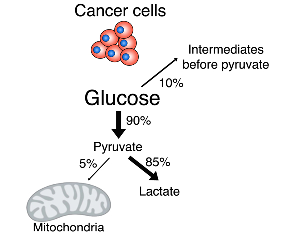
\includegraphics[width=0.5\textwidth]{figs/fig1-4 aerobic glycolysis.pdf}
\caption[Glucose metabolism in cancer cells]{\footnotesize Glucose metabolism in cancer cells. Modified based on Vander Heiden et al. \cite{heiden_understanding_2009}.}
\label{fig:fig1.4}
\end{figure}

Beyond the ATP requirement, cancer cells also need double their cellular contents for the cell division. There are huge needs for nucleotides, amino acids, and lipids for the macromolecular biosynthesis and new membrane formation. Although ATP is indispensable for most of the biomass accumulation reactions, other intermediate metabolites are also needed. For example, the palmitate synthesis for reconstituting new cellular membrane, requires 8 molecules of acetyl-CoA as the carbon source, 14 molecules of NADPH for the reducing power, as well as 7 molecules of ATP. One molecule of glucose could generate up to 36 ATP, or 30 ATP plus 2 NADPH through phosphate pentose pathway, or just provide 6 carbons for macromolecular biosynthesis. Now back to the palmitate synthesis, one molecule of glucose could provide \textasciitilde5 times ATP needed for 16-carbon fatty acid synthesis, or 1/7 of the NADPH needed for it. There is a 35-fold asymmetry between the need for ATP and that for NADPH, given that 3 additional glucose for making the acetyl-CoA as the carbon source for the palmitate synthesis \cite{nelson_lehninger_2013}. Thus, during the cell proliferation, a majority of glucose can not undergo the oxidative phosphorylation to generate ATP, otherwise the resulting high ratio of ATP/ADP will negatively control the flux of glycolysis and compromise the production of acetyl-CoA and NADPH, which leads to the impaired biomass accumulation. The "by-product" lactate could also be converted into glucose again in the liver by the Cori cycle \cite{nelson_lehninger_2013}.


\subsection{Signaling in metabolism reprogramming}

Recently, there were increasing evidences support the hypothesis that the metabolic reprogramming is a hallmark of the tumor development and the primary consequence of the mutation in oncogenes and tumor suppressor genes \cite{hanahan_hallmarks_2011,ward_metabolic_2012}. The cancer cell proliferation not only relies on a large amount of energy consumption, but also needs other build blocks for the cell growth, such as amino acids for the protein synthesis and fatty acids for the lipid bilayer formation. For these purposes, the cell metabolism must undergo a massive reprogramming to fulfill the increased anabolic demand for the cell growth and division. Interestingly, the cancer cell metabolic reprogramming and metabolic syndromes such as type 2 diabetes and hepatosteatosis (fatty liver), are sharing a broad range of signaling pathways in etiology. One of these is the Insulin/PI3K/AKT/mTOR pathway. Activation of PI3K/AKT is probably the most prominent lesion in various types of cancer. mTOR, a downstream target of PI3K/AKT, is well-characterized for its role in enhancing the protein synthesis, glycolysis and lipogenesis via the S6K, HIF1\textalpha{} and SREBP-1 respectively \cite{duvel_activation_2010,hagiwara_hepatic_2012,sun_mammalian_2011}. Dissecting the signaling network behind the insulin signaling could potentially reveal more pharmaceutical targets for treating both cancers and metabolic syndromes. 



\section{Liver metabolism}

The liver is the largest organ in the body, contributing about 2\% total body weight in human and 5\% in mouse \cite{hall_guyton_2010}. The liver is a lobular structure composed of many cylindrical \textit{liver lobules} as the basic function unit. Each unit containing 3 types of cell: hepatocytes, endothelial cells and Kupffer cells (local macrophage cells in the liver). The liver performs many important functions in physiology including:
\begin{inparaenum}[(1)]
\item the filtration and storage of blood
\item the metabolism of carbohydrates, lipids, proteins, hormones and foreign chemicals
\item the bile acid synthesis
\item the vitamin and iron storage
\item the synthesis of serum proteins, such as the albumin, coagulation factors
\end{inparaenum} \cite{hall_guyton_2010}.

In this thesis project, the liver glucose and lipid metabolism are the main focuses. The liver is especially essential organ for maintaining the blood glucose level. The liver can serve as a glucose buffer. In the postprandial phase, a large amount of blood glucose is transported into the liver for the glycogen synthesis and lipid \textit{de novo} synthesis \cite{moore_regulation_2012}, which allow the removal of excess blood glucose and returning into the blood when the glucose level drops below the normal. The liver can also synthesize glucose via gluconeogenesis when blood glucose falls below the normal. During this process, a large amount of amino acids and glycerol released from triglycerides are converted into glucose and released into circulation to maintain the normal level of blood glucose. 

For lipid metabolism, the liver is the major organ for a certain aspect of the fat metabolism, including:
\begin{inparaenum}[(1)]
\item the fat oxidation
\item the synthesis of lipoproteins, cholesterol and phospholipids
\item the free fatty acid and triglyceride synthesis from carbohydrates and proteins
\end{inparaenum} \cite{hall_guyton_2010}. The major sites for \textit{de novo} lipogenesis are the liver and adipose tissues. In the liver, the products from lipogenesis are either stored as lipid droplets in the liver or secreted in the form of \gls{vldl} (\textbf{V}ery \textbf{L}ow \textbf{D}ensity \textbf{L}ipoprotein), which delivers the endogenous derived lipids to peripheral organs.   

\subsection{Liver glucose regulation}

After digestion in the alimentary tract, final products of carbohydrates are glucose, galactose and fructose. Much of the fructose and all of the galactose are interconverted into glucose in the liver. Thus, the glucose becomes the dominant carbohydrate circulating in the blood. 

In the postprandial phase, the liver plays a critical role in nutrient absorption and metabolism, since it is the first barrier to filter all ingested nutrients through the hepatic port vein. This process filters out micro-organisms absorbed together with nutrients, such as bacteria, fungi, viruses and parasites. As the first access to nutrients, the liver is exposed to higher nutrient levels than peripheral organs. A large amount of glycogen is synthesized in the liver in order to relieve the modest hyperglycemia after meal for a normal individual. In addition, the liver also produces glucose to maintain the glucose homeostasis during the fasting state. In a diabetic person, the liver is one of the major culprits for hyperglycemia due to the impaired balance between glucose uptake and production in the liver \cite{krssak_alterations_2004}. 

\subsubsection{Liver glucose uptake}

In the postprandial phase or during the high glucose load via oral or enteral delivery, the liver shifts the balance toward more glucose uptake than endogenous glucose production (\gls{nhgu} (\textbf{N}et \textbf{H}epatic \textbf{G}lucose \textbf{U}ptake) shifts from modest to high in dog \cite{abumrad_absorption_1982,moore_sources_1991}.). Glucose uptake experiments in human and dog have shown that the liver \gls{nhgu} takes up 25--40\% of the administered glucose, while muscle and adipose tissues take one-third, and the non-insulin-sensitive glucose obligating tissues (brain, red blood cells, etc.) absorb the remaining one third (Figure~\ref{fig:fig1.2}). Actually, the liver NHGU underestimates the role of the liver in glycemic control. The total capacity of the liver in glucose disposal upon oral glucose load is about 60--65\%, demonstrates the great importance of the liver in the glucose clearance and production \cite{moore_regulation_2012}. Once taken up by the liver, glucose is converted to glucose-6-phosphate by the liver glucokinase (L-GCK). Unlike other hexokinases, the L-GCK is not inhibited by glucose-6-phosphate. This allows the active glycogen storage in the postprandial phase.

\begin{figure}[htbp]
\centering
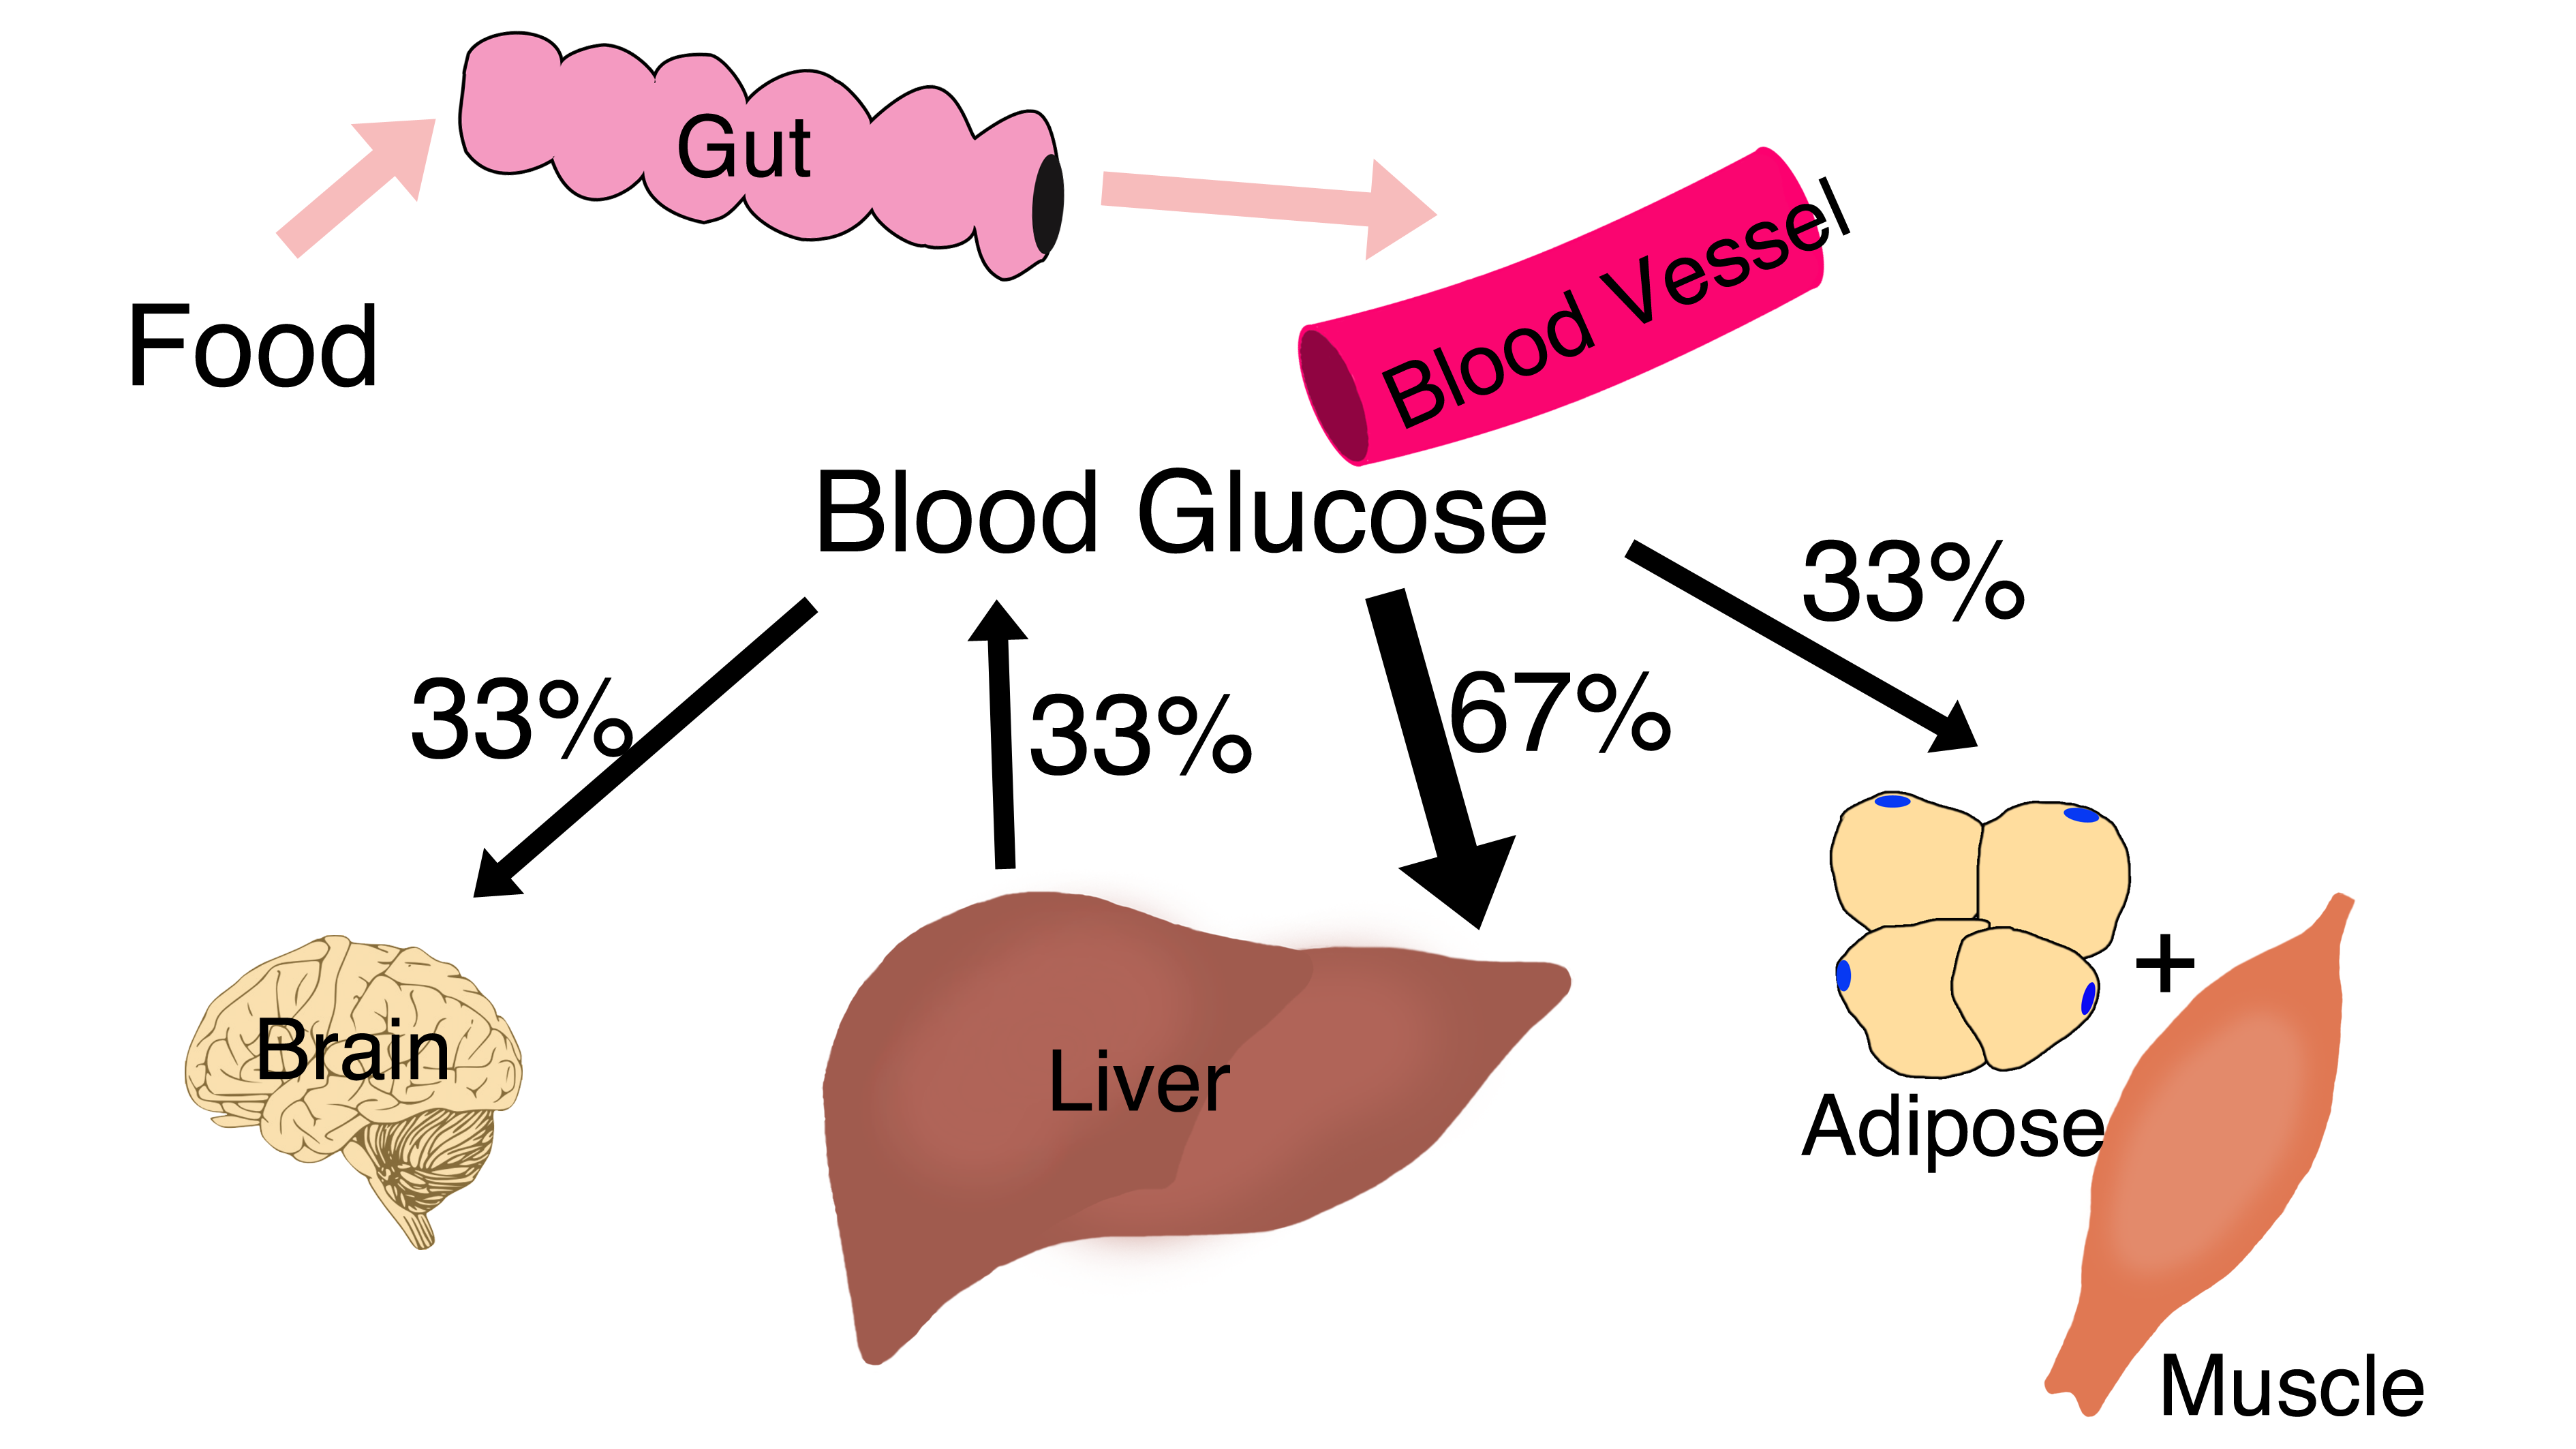
\includegraphics[width=1\textwidth]{figs/fig1-2 liver glucose.png}
\caption[Glucose redistribution in whole body]{\footnotesize Glucose absorption among metabolism related tissues. Modified based on Moore et al. \cite{moore_regulation_2012}.}
\label{fig:fig1.2}
\end{figure}


\subsubsection{Glycolysis for energy and metabolite intermediate production}

Glucose-6-phosphate is further metabolized in glycolysis or stored in the form of glycogen. Glycolysis converts glucose into pyruvate with 2 ATP and 2 NADH released from one glucose molecule. The pyruvate is further decarboxylated to acetyl-CoA and then submitted for the TCA cycle or \textit{de novo} lipogenesis. The pentose phosphate pathway (PPP) is another way of metabolizing glucose, which generates NADPH as the antioxidant or reducing equivalent for the \textit{de novo} lipogenesis and cholesterol synthesis.

\subsubsection{Glycogen storage and breakdown in the liver}

After the glucose is absorbed into the liver, it can be metabolized in glycolytic pathway to release energy and building blocks for the protein and lipid synthesis, or it can be stored as glycogen for future use such as releasing glucose in fasting state. The liver can store as much as 5--8\% of its weight as glycogen. The conversion of glucose to glycogen allows the liver cell store large amount of carbohydrates without increasing the intracellular osmotic pressure.

%\paragraph{Glycogenesis for glycogen formation}
The chemical process of glycogen synthesis is that glucose-6-phosphate is interconverted into glucose-1-phosphate; this is converted to uridine diphosphate glucose, which is finally synthesized into glycogen by glycogen synthase (GS).
%There are several enzymes involved in this process:
%\begin{inparaenum}[(1)]
%\item the phosphoglucomutase for reversible interconversion between glucose-6-phosphate and glucose-1-phosphate;
%\item the UTP-glucose-1-phosphate uridylyltransferase for UDP-glucose synthesis from UTP and glucose-1-phosphate;
%\item the glycogenin for initiating glycogen synthesis by catalyzing the attachment of a glucose molecule to one of its own tyrosine residues;
%\item the glycogen synthase (GS) for catalyzing the elongation of glycogen chains;
%\end{inparaenum}.
The GS can be regulated by several pathways. The glucose-6-phosphate can allosterically activate GS. The phosphorylation of GS can also reduce its activity. Numerous kinases have been shown to regulate GS via phosphorylation \cite{palm_regulation_2013}. The phosphorylation of GS occurs both in the primary and secondary phosphorylation sites. Primary phosphorylation events are initiated by the phosphorylase kinase, \gls{pka}, \gls{AMPK}, \gls{pkc}, \gls{camk2}, and \gls{ck2}. Secondary phosphorylation events are initiated by the \gls{gsk3} and \gls{ck1}. 

%\paragraph{Glycogenolysis for glycogen removal}

In fasting state, the liver produces glucose for the whole body by breaking down glycogen into glucose in a process called glycogenolysis. This process is catalyzed by the glycogen phosphorylase. The glycogen phosphorylase is regulated by the allosteric activation of AMP and activated by the phosphorylation via PKA. The product from glycogenolysis is glucose-1-phosphate, which will be further converted to glucose-6-phosphate by phosphoglucomutase. And the glucose 6-phosphatase remove the phosphate group from glucose-6-phosphate to produce glucose which will be transported out of the liver. 


\subsection{Liver lipid metabolism}

\subsubsection{Dietary lipid absorption}

During the digestion, triglycerides from the food are split into monoglycerides and fatty acids, which are re-esterified in the intestinal epithelial cell into triglycerides and released into the lymphatic system as lipoprotein droplets called chylomicrons (Figure~\ref{fig:fig1.3}). Chylomicrons also contain cholesterol and phospholipids absorbed from the food. The half-life of chylomicrons is less than 1 hour. Most of the chylomicrons are cleared out in the capillary of muscle, adipose and liver by the action of the lipoprotein lipase (LPL). The remnants of chylomicron are absorbed by the liver via the LDL (\textbf{L}ow \textbf{D}ensity \textbf{L}ipoprotein) receptor, LDL receptor-related protein (LRP) and scavenger receptor B-1 mediated endocytosis. The engulfed chylomicrons in hepatocytes are digested in the lysosome to release glycerol, fatty acids, cholesterol, which are recycled into VLDL.



\subsubsection{Lipoprotein particle for lipid transportation and redistribution}

Besides chylomicrons, there are four major types of lipoprotein particles circulating in the plasma (Figure~\ref{fig:fig1.3}). Most of these lipoprotein particles are synthesized by the liver and employed to redistribute triglycerides, cholesterols, and phospholipids among peripheral tissues. These lipoprotein particles are classified based on their density measured in the ultracentrifugation:
\begin{inparaenum}[(1)]
\item the \gls{vldl} is synthesized in the liver and containing the highest amount of triglycerides (\textasciitilde70\%) and modest amount of cholesterol (\textasciitilde7.5\%) and phospholipids \cite{ginsberg_regulation_2005};
\item the \gls{idl} (\textbf{I}ntermediate \textbf{D}ensity \textbf{L}ipoprotein) is derived from the VLDL, in which triglycerides are partially removed;
\item the \gls{ldl} is derived from the IDL, in which almost all triglycerides are absorbed by peripheral tissues, left with very high amount of cholesterol (\textasciitilde45\%) \cite{ginsberg_regulation_2005};
\item the \gls{hdl} (\textbf{H}igh \textbf{D}ensity \textbf{L}ipoprotein) is synthesized in the liver or intestine epithelium, containing high concentration of protein (\textasciitilde50\%) and modest amount of cholesterols (\textasciitilde20\%) and phospholipids \cite{ginsberg_regulation_2005};
\end{inparaenum}.

\begin{figure}[!tb]
\centering
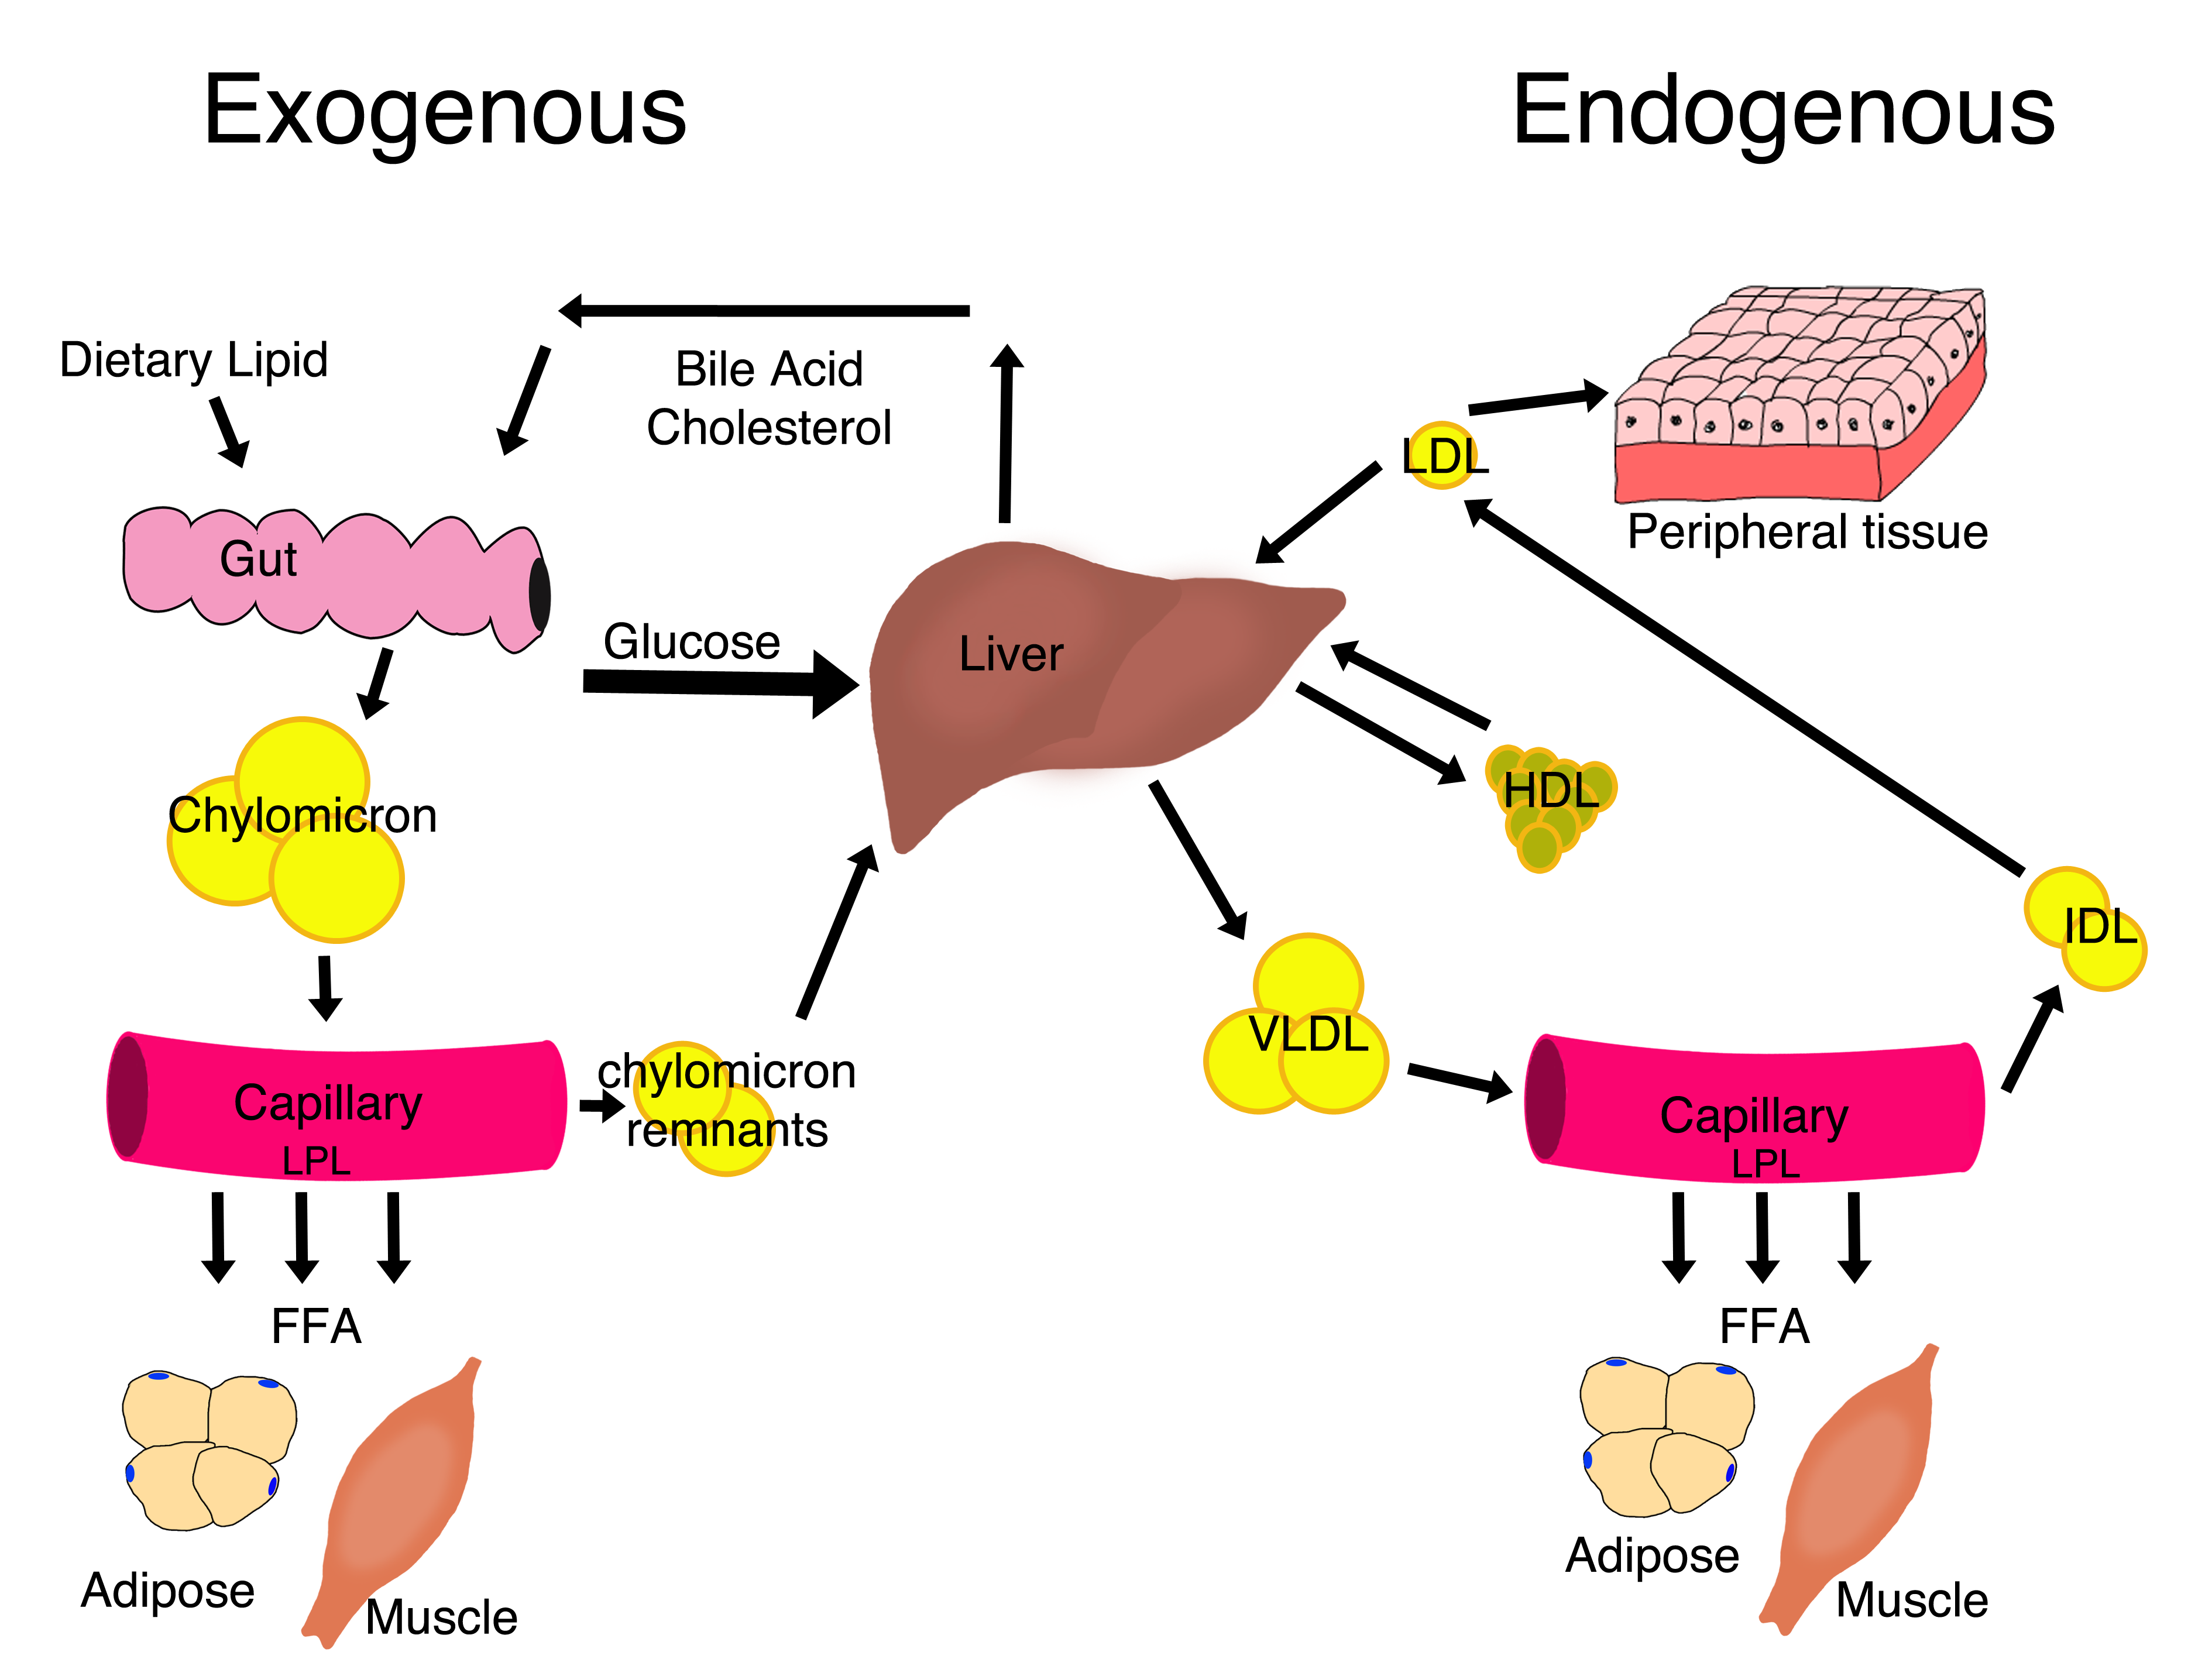
\includegraphics[width=1\textwidth]{figs/fig1-3 liver lipid.png}
\caption[Lipid redistribution in the whole body]{\footnotesize The lipid absorption and lipoprotein particle redistribution among metabolism related tissues.}
\label{fig:fig1.3}
\end{figure}

In contrast to the chylomicron for exogenous lipid transportation, the primary function of the VLDL is transporting endogenous liver-derived triglycerides and cholesterols to peripheral tissues such as the muscle and adipose tissues. As partially digested lipoprotein from VLDL, the IDL is either taken up by the liver or continually circulating in the plasma to convert into LDL. The LDL contains high amount of cholesterol, which is also called the "bad cholesterol" in comparison to the "good cholesterol" in HDL. Increasing blood cholesterol from LDL is a strong risk factor for causing the atherosclerosis. The HDL is responsible for the delivery of the cholesterol to peripheral tissues and the removal of excess cholesterol from the plasma in a process called the reverse cholesterol transport \cite{mahley_putting_2006,van_der_velde_reverse_2010}.

\subsubsection{\textit{de novo} lipogenesis in the liver}

Whenever a greater amount of the carbohydrate than it can be used immediately such as in glycolysis or stored in the form of glycogen, the excess is quickly converted to triglycerides. Most of the triglyceride synthesis occurs in the liver, while a small fraction also occurs in the adipose tissue. The hepatic \textit{de novo} lipogenesis include the fatty acid synthesis from the acetyl-CoA and malonyl-CoA, and further synthesis of triglycerides. The fatty acid synthesis is catalyzed by the acetyl-CoA carboxylase for the malonyl-CoA synthesis and the fatty acid synthase for the fatty acid elongation up to 16 carbons. The fatty acid and its metabolites are the major culprits for lipotoxicity. Thus, fatty acids are quickly further stored as triglycerides, which are relatively inert and shown to have a hepatic protective role \cite{choi_hepatic_2008}. The triglyceride synthesis starts from the glycerol-3-phosphate and fatty acid-CoA by the glycerol-3-phosphate acyltransferase (GPAT) to form the lysophosphatidic acid, then further adding fatty acids stepwise by the acylglycerolphosphate acyltransferase (AGPAT), phosphatidic acid phosphohydrolase (PAP) and diacylglycerol acyltransferase (DGAT) to have triglycerides. Finally, triglycerides are packaged into the VLDL. 

\subsubsection{\texorpdfstring{\textbeta}{b}-oxidation of fatty acids}

The degradation and oxidation of fatty acids occur in mitochondria, peroxisomes and ER \cite{bechmann_interaction_2012}. For the \textbeta{}-oxidation in mitochondria, fatty acids are first transported via the help from the carrier called carnitine. Then fatty acids in mitochondria are progressively processed to release the acetyl-CoA and reducing equivalent such as FADH\textsubscript{2} and NADH. The \textbeta{}-oxidation of fatty acid will release a tremendous amount of energy from it. For example, one molecule of stearic acid will release net gain of 146 molecules of ATP after complete oxidation \cite{hall_guyton_2010}. The acetyl-CoA can also be converted to the ketone body in case of excess fatty acid, or further processed in the TCA cycle. Two acetyl-CoA can be condensed into one acetoacetic acid. The acetoacetic acid can also be converted to the \textbeta{}-hydroxybutyric acid \cite{nguyen_liver_2008}. In ER, long-chain fatty acids can be degraded via the \textomega{}-oxidation by the cytochrome P450 \cite{reddy_nonalcoholic_2001}. PPAR\textalpha{} and insulin are the positive and negative regulator for the fatty acid oxidation \cite{bechmann_interaction_2012}.

The formation of ketone bodies, which is also called the ketogenesis, is mainly happening in the liver cell mitochondrial matrix when blood glucose level is low and the liver has to provide extra energy for other organs, such as the muscle, heart and brain. After its production in the liver, the water soluble ketone body species are released into the blood, and transported into other organs where the acetoacetic acid and \textbeta{}-hydroxybutyric acid can be re-converted into the acetyl-CoA as the energy source. 


\section{PP2A and its biology}

The reversible protein phosphorylation is one of the most abundant post-translational modifications (PTMs), in which the protein residue serine/threonine/tyrosine is phosphorylated by kinases and de-phosphorylated by phosphatases. The regulation of protein phosphorylation is considered to be one of the most common way of the protein function regulation, which switches protein between the active and inactive form, or between the stabilization and degradation, or different cellular localizations \cite{ptacek_charging_2006,pawson_protein_2005,cohen_regulation_2000}. While the previous basic research and pharmaceutical development is mainly focused on the kinase activity modulation to affect the protein phosphorylation, it is now also being recognized that the protein phosphatase could also be an important regulator in the protein phosphorylation and provide the new drug candidate to change the protein phosphorylation pharmacologically \cite{newton_turning_2014,khanna_cancerous_2013,chatterjee_targeting_2013,de_munter_challenges_2013,dadke_protein-tyrosine_2003}. 

\subsection{PP2A structure}

The protein phosphatase 2 (PP2A) is a heterotrimeric serine/threonine phosphatase with broad substrate specificity and diverse cellular functions. The PP2A is composed of a dimeric core enzyme formed by a scaffold A subunit and a catalytic C subunit, and a regulatory B subunit for expanding PP2A's substrate specificity. While the A and C subunit sequence have extraordinary sequence conservation throughout eukaryotes, the regulatory B subunits show more heterogeneous sequence evolution. This indicates a highly conserved core enzyme functionality of the PP2A during evolution, but continuous evolution on the B subunit for expanding substrate specificity constantly. 
%latex.default(tab1.2, rowname = NULL)%
\begin{table}[!t]
\begin{center}
\begin{threeparttable}
\caption[PP2A gene superfamily]{PP2A gene superfamily composition\tnote{a}.}
\label{tab:tab1.2}
\begin{footnotesize}
\begin{tabular}{lll}
\toprule
\multicolumn{1}{c}{Subunit}&\multicolumn{1}{c}{Gene Name}&\multicolumn{1}{c}{Protein Name}\tabularnewline
\midrule
\multirow{2}{*}{PP2A-A}&PPP2R1A&PR65\textalpha\tabularnewline
&PPP2R1B&PR65\textbeta\tabularnewline
\midrule
\multirow{2}{*}{PP2A-C}&PPP2CA&PP2Ac\textalpha\tabularnewline
&PPP2CB&PP2Ac\textbeta\tabularnewline
\midrule
\multirow{4}{*}{PP2A-B}&PPP2R2A&PR55\textalpha\tabularnewline
&PPP2R2B&PR55\textbeta\tabularnewline
&PPP2R2C&PR55\textgamma\tabularnewline
&PPP2R2D&PR55\textdelta\tabularnewline
\midrule
\multirow{5}{*}{PP2A-B\textsuperscript{$\prime$}}&PPP2R5A&PR56/61\textalpha\tabularnewline
&PPP2R5B&PR56/61\textbeta\tabularnewline
&PPP2R5C&PR56/61\textgamma\tabularnewline
&PPP2R5D&PR56/61\textdelta\tabularnewline
&PPP2R5E&PR56/61\textepsilon\tabularnewline
\midrule
\multirow{5}{*}{PP2A-B\textsuperscript{$\prime\prime$}}&PPP2R3A&PR130, B\textsuperscript{$\prime\prime$}\textalpha{}1\tabularnewline
&PPP2R3A&PR72, B\textsuperscript{$\prime\prime$}\textalpha{}2\tabularnewline
&PPP2R3B&PR70, B\textsuperscript{$\prime\prime$}\textbeta\tabularnewline
&PPP2R3C&G5PR\tabularnewline
&PPP2R3D&PR59, B\textsuperscript{$\prime\prime$}\textdelta\tabularnewline
\midrule
\multirow{3}{*}{PP2A-B\textsuperscript{$\prime\prime\prime$}}&STRN&Striatin/PR110\tabularnewline
&STRN3&SG2NA/PR93\tabularnewline
&PPP2R4&PR53\tabularnewline
\bottomrule
\end{tabular}
\end{footnotesize}
\begin{tablenotes}  
\item[a] \scriptsize{Adapted from Perrotti et al. \cite{perrotti_protein_2013}}.
\end{tablenotes}
\end{threeparttable}
\end{center}
\end{table}

Multicellular eukaryotes are believed to express four classes of regulatory subunits: B, B$^{\prime}$, B$^{\prime \prime}$, and B$^{\prime \prime \prime}$ , with at least 17 members in these different subfamilies (Table~\ref{tab:tab1.2}). Beyond this layer of complexity in the gene family, each gene can also have various splicing isoforms. In total, different combinations of certain isoform of certain gene subfamily member provide more than 200 possible variations of the PP2A. This will also explain why phosphatases, even less represented than kinases in the genome, can counteract the phosphorylation events by many kinases. The Table~\ref{tab:tab1.1} shows the unbalanced number of genes for phosphatases and kinases in different genome, from Yeast to Human.

%latex.default(tab1.1, rowname = NULL)%
\begin{table}[!b]
\begin{center}
\begin{threeparttable}
\caption[Kinase/phosphatase gene number]{Kinase/phosphatase gene number imbalance in genome\tnote{a}.}\label{tab:tab1.1}
\begin{footnotesize}
\begin{tabular}{p{0.25\textwidth}cccP{0.22\textwidth}}
\toprule
\multicolumn{1}{c}{Gene Family}&\multicolumn{1}{c}{\textit{S. cerevisiae}}&\multicolumn{1}{c}{\textit{D. melanogaster}}&\multicolumn{1}{c}{\textit{C. elegans}}&\multicolumn{1}{c}{\textit{H. sapiens}}\tabularnewline
\midrule
Total Gene Number&$6122$&$13600$&$18988$&25000\tabularnewline
Total Protein Kinase Number&$ 124$&$  236$&$  493$&518\tabularnewline
Total Protein Phosphatase Number &$  37$&$   93$&$  185$&119 (21 Protein S/T Phosphatase)\tabularnewline
\bottomrule
\end{tabular}
\end{footnotesize}
\begin{tablenotes}  
\item[a] \scriptsize{Adapted from Seshacharyulu et al. \cite{seshacharyulu_phosphatase:_2013}}.
\end{tablenotes}   
\end{threeparttable}
\end{center}
\end{table}

\subsubsection{PP2A catalytic subunit}

Mammalian \gls{PP2A} catalytic subunit (PP2A-C) is a metallophosphatase, which requires normally the Mg\textsuperscript{2+} in its active center for catalytic activity. The PP2A-C subunit is encoded by two gene subfamily members, \textalpha{} and \textbeta{}, which share 97\% amino acid sequence identity with only minor difference at the beginning N-terminal. The two sub-members of PP2A-C are differentially expressed. The PP2A-C\textsubscript{\textalpha} is about 10 times more efficiently transcribed than the PP2A-C\textsubscript{\textbeta} \cite{khew-goodall_tissue-specific_1988}, probably due to the higher expression capacity of the PP2A-C\textsubscript{\textalpha} promoter \cite{khew-goodall_structure_1991}. The overexpression of PP2A-C in mammalian cell was not successful. And the knockout mouse of PP2A-C\textsubscript{\textalpha} was not viable and die at embryonic 6.5 day \cite{gotz_delayed_1998}, which indicated the importance of PP2A-C\textsubscript{\textalpha} in the mouse development and its non-redundancy in term of rescuing by PP2A-C\textsubscript{\textbeta}.

\subsubsection{PP2A scaffold subunit}

The scaffold A subunit is also encoded by two distinct isoforms, PP2A-A\textsubscript{\textalpha} and PP2A-A\textsubscript{\textbeta}, which share 86\% sequence identity. The A subunit is the structural subunit which provides scaffold for the association of regulatory B subunit and catalytic C subunit. Since the different regulatory subunit binds with the same or overlapping surface on the A subunit, the association of regulatory subunit to the holoenzyme is mutually exclusive \cite{cho_crystal_2007,ruediger_molecular_1994}. This structural characteristic in PP2A defines the existence of potential PP2A sub-pool and diversified substrate specificity. 
Mice that are homozygous for PP2A-A\textsubscript{\textalpha} knockout are embryonic lethal \cite{ruediger_human_2011}. The oocyte-specific knockout of PP2A-A\textsubscript{\textalpha} leads to severe defect in the female meiosis and fertility in mice \cite{hu_scaffold_2014}. The mouse knock-in model of human cancer-associated mutations in PP2A-A\textsubscript{\textalpha} increases the lung cancer incidence and indicates its potential tumor suppressor function \cite{ruediger_human_2011}. 

\subsubsection{PP2A regulatory subunit}

Regulatory subunits of PP2A are diverse (Table~\ref{tab:tab1.2}) and low in sequence similarity between these four gene families, even though they all bind to similar repeats in the A subunit. From the crystal structure, it was postulated that the regulatory subunit, together with the catalytic subunit, establish the binding groove for substrates \cite{xing_structure_2006}. The diversity of regulatory subunit can partially explain how PP2A counteracts phosphorylation from multiple kinases by having diversified substrate recognition. 

The PP2A-B gene family has four sub-members (Table~\ref{tab:tab1.2}). The PR55\textalpha{} and PR55\textdelta{} are expressed in almost all tissues, while the PR55\textbeta{} and PR55\textgamma{} are highly expressed in the brain \cite{janssens_protein_2001}. Structurally, the PP2A-B family protein's common feature is the existence of 5 degenerated \gls{wd40} repeats, which are believed to be involved in protein-protein interactions.

The PP2A-B\textsuperscript{$\prime$} gene family currently contains 5 member (Table~\ref{tab:tab1.2}). While the PR61\textalpha{}, PR61\textbeta{} and PR61\textepsilon{}  are mainly localized in cytoplasm, the PR61\textgamma{} and PR61\textdelta{} are localized both in cytoplasm and nucleus. For tissue expression pattern, the PR61\textalpha{} and PR61\textgamma{} are expressed in almost all tissues, especially high in the heart and skeletal muscle. And  the PR61\textbeta{} and PR61\textdelta{} are highly enriched in the brain \cite{csortos_high_1996,tehrani_identification_1996,tanabe_molecular_1996}. All PP2A-B\textsuperscript{$\prime$} genes share a conserved central region (80\% identical), with different C and N terminal. This indicates the central region is probably more involved in the association with the scaffold and catalytic subunit, while the C and N terminal could be involved in regulating substrate diversity. 

Initially, the PR72 and PR130 were discovered as founding members of PP2A-B\textsuperscript{$\prime\prime$} \cite{hendrix_structure_1993}. The only sequence difference between them is located at N terminal, which raises the possibility that PR72 and PR130 are originated from alternative splicing. Two other member PR48 and PR59 are discovered by the yeast two-hybrid as interaction partners for the retinoblastoma-related p107 protein and Cdc6 respectively \cite{voorhoeve_functional_1999,yan_pr48_2000}.

The PR93 and PR110 are discovered as members of PP2A-B\textsuperscript{$\prime\prime\prime$} family based on their sequence conservation with PP2A-B\textsuperscript{$\prime$} family. These two proteins are all calmodulin-binding protein and suggesting their associated PP2A holoenzyme are involved in the calcium-dependent signaling \cite{moreno_wd40_2000}.

\subsection{PP2A in signaling}

PP2A is essential to the majority of signaling pathways, including cell cycle control, Wnt signaling, insulin signaling, apoptosis, cell adhesion and cytoskeleton dynamics, etc. (Details in Figure~\ref{fig:fig1.1}). The mis-regulation of PP2A complex will influence on a lot of, if not all, physiological processes. 

\begin{figure}[!ht]
\centering
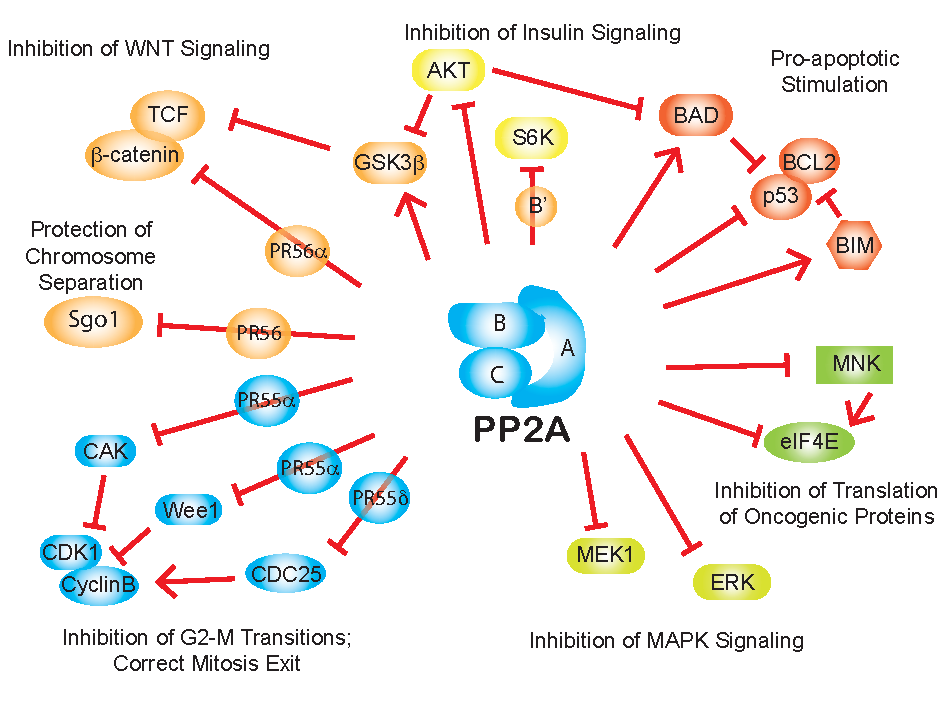
\includegraphics[width=1\textwidth]{figs/fig1-1 pp2a signaling.pdf}
\caption[PP2A in signaling]{\footnotesize PP2A is involved in many signaling pathways by counteracting phosphorylation events by many kinases. Adapted from Perrotti et al. \cite{perrotti_protein_2013}.}
\label{fig:fig1.1}
\end{figure}

\subsubsection{PP2A in metabolism}

Multiple PP2A regulatory subunits have been demonstrated to be involved in regulating the metabolism via the Insulin/\gls{akt}/\gls{mtor} signaling pathways. In \textit{Drosophila}, Hahn et al. demonstrated that PP2A regulatory B\textsuperscript{$\prime$} target S6K to modulate the phosphorylation of its activation site in our lab, and this regulation was conserved even in the Hela cell line \cite{hahn_pp2a_2010}. Another \textit{Drosophila} B\textsuperscript{$\prime$} subunit Widerborst modulates activated AKT via direct interaction and change the lipid droplet size and expression of lipid storage protein perilipin \cite{vereshchagina_protein_2008}. The C. \textit{elegans} B\textsuperscript{$\prime$} subunit pptr-1 could also directly regulate AKT's phosphorylation \textit{in vivo} and impact the life span, fat storage phenotype of worms \cite{padmanabhan_pp2a_2009}. 

In the mammalian system, AKT was also found to be associated with the PP2A--B55 holoenzyme, and its phosphorylation at Thr--308 was compromised by overexpressing PR55\textalpha{} subunit in both FL5.12 and NIH3T3 cells \cite{kuo_regulation_2008}. In 3T3-L1 adipocytes, over-expression of small t antigen, which generally inhibits PP2A activity, was found to have multiple impacts on the insulin pathway, including increased phosphorylation of insulin signaling downstream effector--AKT and GSK-3\textbeta{} \cite{ugi_protein_2004}. The inhibition of PP2A by the small t antigen in 3T3-L1 adipocytes enhanced the glucose uptake both in basal and insulin-stimulated condition. Another important master regulator in metabolism, the AMPK, was also found to be negatively regulated by PP2A \cite{wu_activation_2007,park_ampk_2013,wang_pp2a_2010}. In HepG2 cells, heat shock stress will dephosphorylate AMPK and enable to relieve the AMPK-mediated suppression on HSP70 expression \cite{wang_pp2a_2010}. And the AMPK inhibition after heat shock stress was shown to be mediated by PP2A. Intracellular calcium or palmitate could also inactivate AMPK via PP2A. The PP2A-B\textsuperscript{$\prime\prime$} subunit PR72 is known to have calcium binding sites, and could potentially be involved in intracellular calcium-mediated AMPK inhibition \cite{park_ampk_2013}. Excess fatty acid treatment, such as palmitate, could also inactivate AMPK via PP2A \cite{wu_activation_2007}.   

\subsubsection{PP2A in Wnt signaling}

In \textit{Xenopus}, B\textsuperscript{$\prime$} subunit PR56\textalpha{} was discovered to the negative regulator for the \textbeta-Catenin phosphorylation, which lead to the degradation of \textbeta-Catenin via the ubiquitin/proteasome pathway \cite{li_protein_2001}. However, recent evidences showed the PP2A has more complicated control in Wnt signaling \cite{eichhorn_protein_2009}. Before Wnt ligand binding, \textbeta-Catenin is located in destruction complex including \gls{apc}, AXIN, and GSK3\textbeta{}. The PP2A B subunits, PR61\textalpha{}-\textdelta{}, binds to either APC or AXIN to destabilizing the \textbeta-Catenin. However the mechanism is still not clear. Upon Wnt ligand binding, the Wnt downstream effector Naked, which causes a negative feedback on Wnt signaling, requires the PR72 for its negative regulation, and is repressed by the PR130 (alternative splicing form of the PR72). Additionally, both PR61\textepsilon{} and PR55 could enhance Wnt signaling by destabilizing the inhibitory GSK3\textbeta{} (Figure~\ref{fig:fig1.1}). 

\subsubsection{PP2A in MAPK signaling}

For MAPK kinase signaling cascades, PP2A has also both inhibitory and activating role \cite{eichhorn_protein_2009}. Depending on the different combination of PP2A complexes, almost all MAPK pathways can be negatively regulated \cite{junttila_phosphatase-mediated_2008}. Both \textit{in vivo} and \textit{in vitro} studies has shown that inhibition of PP2A increases ERK and MEK phosphorylation \cite{junttila_phosphatase-mediated_2008}. Furthermore, PR61\textbeta{} and PR61\textgamma{} directly de-phosphorylate ERK \cite{eichhorn_protein_2009} (Figure~\ref{fig:fig1.1}). PP2A was also shown to interact with Shc, the upstream regulator in MAPK signaling, and suppress its tyrosine phosphorylation and activation on MAPK signaling cascade \cite{junttila_phosphatase-mediated_2008}. 

Related to PP2A's activating role, PR55\textalpha{} binds and de-phosphorylates KSR1 and RAF upon RAS activation. And this leads to the plasma membrane recruitment of RAF and subsequent enhanced binding between RAF and RAS, therefore stronger activation of MAPK signaling \cite{eichhorn_protein_2009}. On the other hand, PR55\textgamma{} interacts with c-SRC and inhibits c-SRC's positive regulation on RAF independently from RAS activation. 


\subsubsection{PP2A in apoptosis}

PP2A has also pro-apoptotic activity via its inhibitory effect on AKT, which inactivates the anti-apoptotic protein BCL2 and activates pro-apoptotic factors like BAD and BIM \cite{eichhorn_protein_2009,janssens_role_2012} (Figure~\ref{fig:fig1.1}). PP2A directly binds BCL2 and BIM and de-phosphorylates them. Also, PP2A directly binds to the BH4 domain of BCL2 and removes the phosphorylation at Ser70 of BCL2, which causes enhanced interaction between p53 and BCL2 to inhibit BCL2's anti-apoptotic function. Additionally, the inhibition of PP2A by okadaic acid or siRNA increases eIF4E phosphorylation via MNK kinase \cite{li_protein_2010}. These findings are consistent with the tumor suppressor role of PP2A.


\subsubsection{PP2A in cell cycle control}

PP2A has a fundamental role in controlling cell cycle. During G1--S transition, PR56\textgamma{} is translocated into the nucleus and PP2A terminal methylation levels also change \cite{eichhorn_protein_2009}. Also, PR55\textalpha{} is inhibiting CDK1-Cyclin B complex via the inhibition of \gls{cak} and Wee1 kinase. PR56\textdelta{} could also de-phosphorylate CDC25 and inactivate it. The PR56 family could also regulate sister chromatid cohesion, which is important for proper chromosome segregation in mitosis and meiosis \cite{hu_scaffold_2014,kitajima_shugoshin_2006}. In my own PhD thesis project, over-expression of mouse PP56\textgamma{} (PPP2R5C) in Hepa 1-6 has also resulted in dense chromosome in \gls{dapi} staining, which confirmed the B\textsuperscript{$\prime$} subunits' role in chromosome segregation (data not shown). 


\subsubsection{PP2A in cell proliferation}

PP2A has been demonstrated with multiple evidences for its tumor suppressor activity in the human cell transformation \cite{janssens_pp2a:_2005,mumby_pp2a:_2007}. Viral antigen SV40 small T antigen or tumor-inducing toxins like okadaic acid and microcystin-LR have been shown to be the viral or chemical inhibitor for PP2A activity \cite{campbell_identification_1995,nagao_protein_1995}. In addition, \textit{in vivo} inhibitor for PP2A CIP2A, an endogenous interacting protein for PP2A, has been found to be the stabilizer for c-Myc and mediating PP2A's inhibition in human malignancies \cite{khanna_cancerous_2013,junttila_cip2a_2007}. 

PP2A scaffold and regulatory subunits have been shown to be mutated or down-regulated in multiple cancers \cite{seshacharyulu_phosphatase:_2013}. Knockdown of PR56\textgamma{} in HEK cell inhibits PP2A phosphatase activity similar to the extent achieved by SV40 small T antigen and induces anchorage-independent tumor growth \cite{chen_identification_2004}. The PP2A PR56\textgamma{} containing holoenzyme has tumor growth suppression activity via de-phosphorylation on the p53 at Thr--55 \cite{li_specific_2007,shouse_serine_2008}, and leads to the growth arrest and inhibition of cell proliferation.

\section{Aim of study--PPP2R5C}

In our lab, homolog of PPP2R5C in Drosophila, \gls{PP2A}-B\textsuperscript{\ensuremath{\prime}}, has been previously shown that it regulates the organismal metabolism \cite{hahn_pp2a_2010} via directly de-phosphorylating \gls{s6k} in \textit{Drosophila}. In agreement with S6K activation phenotype, fly with \gls{PP2A}-B\textsuperscript{\ensuremath{\prime}} whole body knockout had increased insulin signaling phenotype, which was the decreased life span and whole body triglyceride. The initial study in Hela cell also shows that the human homolog of \gls{PP2A}-B\textsuperscript{\ensuremath{\prime}}, PPP2R5C, also negatively regulates the S6K phosphorylation. The naturally following question would be whether there is any link between PPP2R5C and metabolic status in more translational related context, such as in mice or human patients. 

The knockout mice in PPP2R5C results in heart development defects, including the formation of incomplete ventricular septum and a decrease in the number of ventricular cardiomyocytes \cite{varadkar_protein_2014}. In addition, PPP2R5C knockout mice have a decrease in locomotive coordination and gripping strength, which indicates that PPP2R5C is also required for efficient neuromuscular function. Finally, the knockout mice have also neonatal growth deficiency, but survived knockout mice develop obesity after weaning and have 31\% more body weight at the age of 6 months. However, the exact mechanism causing the obesity is still not clear. It could be a secondary consequence of reduced locomotive activity or active metabolic change in a certain metabolic relevant organ. The tissue-specific manipulation of PPP2R5C is needed for clarifying the multiple defects in whole-body knockout mice. 

Proteomic studies on PPP2R5C interacting partners reveals several interesting candidates as PPP2R5C's phosphatase substrates \cite{arroyo_liprin_2008,zhou_proteomic_2007}. A \gls{gst} tagged PPP2R5C was used to unravel its potential interaction partners by Mass Spectrometry approach \cite{zhou_proteomic_2007}. And several proteins, such as the calcium pump SERCA2a and SERCA3a, are involved in the calcium homeostasis. Interestingly, the SERCA2a has been recently identified as the Serpin-interacting protein and shown that SERCA2a homolog in \textit{Drosophilla} is required for the fat storage in fat body (primitive organ with function of the liver and adipose tissue in \textit{Drosophilla} \cite{hietakangas_regulation_2009}) \cite{bi_seipin_2014}, which could potentially be conserved in mice and fit with the obesity phenotype in PPP2R5C knockout mice \cite{varadkar_protein_2014}. The over-expression of PPP2R5C in cultured myocytes impairs the cell contractility \cite{zhou_proteomic_2007}. Another \gls{tap} tagged PPP2R5C based proteomic strategy also found the Liprin \textalpha{}1 is interacting with PPP2R5C independent of PP2A holoenzyme \cite{arroyo_liprin_2008}. Liprin \textalpha{}1 is suggested to stabilize PPP2R5C and regulate the focal adhesion \cite{arroyo_liprin_2008}. 

Human PPP2R5C has been shown to be involved in regulating p53 tumor suppressor activity upon DNA damage\cite{li_specific_2007,shouse_serine_2008}. After DNA damage, the PR56\textgamma{} containing PP2A holoenzyme binds p53 and de-phosphorylates Thr55 of p53, which leads to the induction of downstream transcriptional target p21 and following inhibition of cell proliferation \cite{li_specific_2007}. In addition, the interaction between PR56\textgamma{} and p53 upon DNA damage require the ATM-dependent phosphorylation of Ser15 in p53 \cite{shouse_serine_2008}. However, p53 protein sequence alignment between human and mouse shows that the Thr55 in mouse is missing, and this deletion rules out the possibility of mouse PR56\textgamma{}'s ability to inhibit the cell proliferation via p53. Indeed, PPP2R5C knockdown in mouse cell lines has very mild effects on proliferation (\textit{circa} 5\% increase in total protein content, data not shown).

Human PPP2R5C is also involved in \gls{tcr}-induced \gls{nfkb} activity \cite{breuer_protein_2014}. The \gls{nfkb} is activated upon T cell stimulation by complex phosphorylation event cascade. PPP2R5C was found to be the negative regulator to fine-tune and terminate the \gls{nfkb} activation. PPP2R5C silencing in stimulated primary human T cell causes increased phosphorylation in \gls{ikk} and \gls{ikba}. 

In this thesis project, I have explored the mammalian function of PPP2R5C in metabolism control by tissue-specifically manipulating the expression of PPP2R5C in metabolically relevant tissues, such as the mouse liver. In addition, I have also employed systematic approaches, such as the microarray analysis after PPP2R5C knockdown and the proteomic study of PPP2R5C's substrates, to investigate the potential mechanism behind PPP2R5C's metabolism control. 




\chapter{Results}\label{result}
% !TEX encoding = UTF-8 Unicode

\section[Transcriptional change of PPP2R5C]{Transcriptional change of PPP2R5C in response to metabolic state or diseases}

\subsection{PPP2R5C splicing isoforms}

In mice, PPP2R5C gene contains 4 splicing isoforms  according to the NCBI's genbank annotation when I started the project. Initially, they were annotated as PPP2R5C Variant 1--4 (named Variant 1--4 in the following sections). Now with deeper annotation, there are 11 different isoforms for the mouse PPP2R5C annotated in NCBI. The gene structure is shown in Figure~\ref{fig:fig2.0}. Various isoforms of PPP2R5C shares the central exons while differs at both N and C terminal. From the structure of B56 containing PP2A holoenzyme \cite{cho_crystal_2007,xing_structure_2006}, it is reasonable to postulate that central region of PPP2R5C is more involved in the association to PP2A A and C subunit while the N and C terminal are more engaged in fine-tuning the substrate specificity among isoforms. 

\begin{figure}[htbp]
\centering
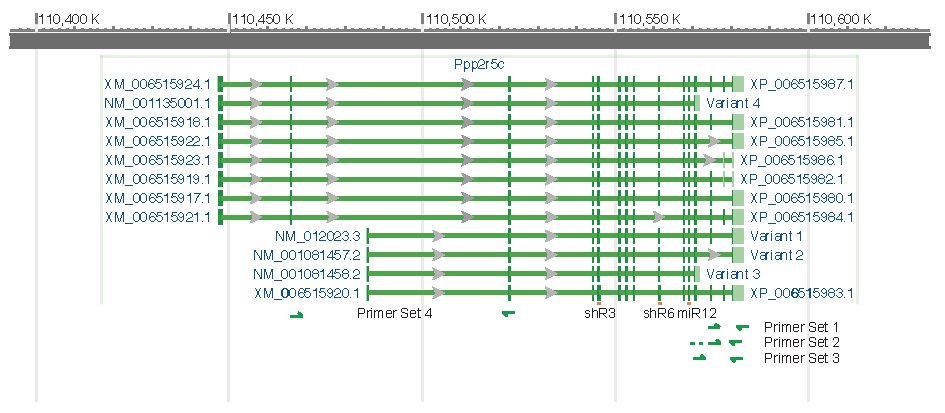
\includegraphics[width=1\textwidth]{figs/fig2-0 ppp2r5c gene structure.pdf}
\caption[Mouse PPP2R5C gene structure]{\footnotesize Mouse PPP2R5C gene structure. Four splicing isoforms, Variant 1 to 4, are displayed with exons and introns according to NCBI genbank annotation. Primer sets for Variant 1--4 are also shown in their corresponding positions. miRNAs/shRNAs targeting the common region of all isoforms, including shR3, shR6 and miR12, are also shown at their relative positions. Adapted from NCBI genbank record of mouse PPP2R5C.}
\label{fig:fig2.0}
\end{figure}

\subsection{Transcriptional change of PPP2R5C in response to metabolic state}

Since genes for metabolic regulators are often present in regulatory transcriptional feedback loops \cite{amemiya-kudo_promoter_2000}, I tested the relationship between the PPP2R5C expression and organismal nutritional status in various mice tissue samples by qPCR. Indeed, obese mice lacking the leptin receptor (\textit{db/db}) have significantly elevated levels of various PPP2R5C mRNA isoforms in the liver (Figure~\ref{fig:fig2.1}). By the \gls{ANOVA} (Analysis of Variance) analysis, at least for Variant 1, 2 and 4, there are significant increases in the transcriptional level of PPP2R5C in the \textit{db/db} mice liver comparing with the \textit{wt/wt} mice. The Variant 3 has also shown a similar trend through not significant. However, the total protein level of PPP2R5C, measured by home-made antibody (Section~\ref{sec:sec222}) for the mouse PPP2R5C, did not show a significant increase in the protein level. %This discrepancy in the mRNA and protein level of PPP2R5C further indicates the up-regulation in \textit{db/db} is a transcriptional feedback.

\begin{figure}[!tb]
\centering
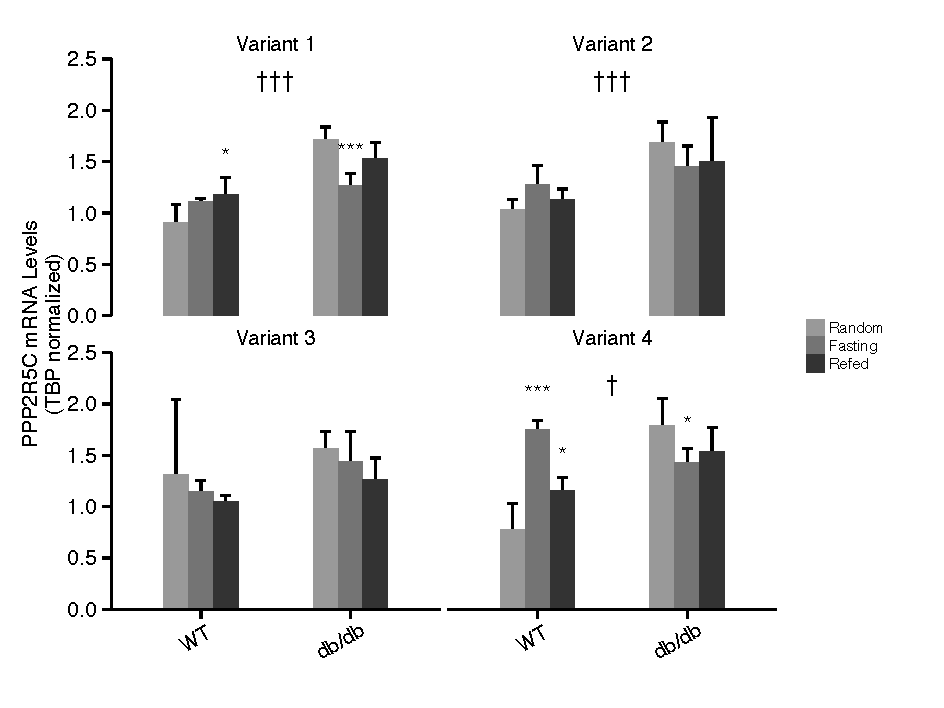
\includegraphics[width=1\textwidth]{figs/fig2-1 liver ppp2r5c.pdf}
\caption[PPP2R5C expression in the liver]{\footnotesize PPP2R5C is regulated in the mouse liver. Mouse PPP2R5C transcript variant 1--4 mRNA levels in the liver from 8-12 week C57BL/6 wild type (WT) or \textit{db/db} male mice under different nutritional statuses are shown here. Mice were fed with the normal chow diet without limit ("Random"). For "Fasting" and "Refed", mice were first starved for 16 hours and then allowed to the normal chow diet access for 6 hours. Error bar: std. dev. (this is the same for all following figures with error bars). * and *** for p-value<0.05 and 0.001 by the t-test within each mice genotype (WT or \textit{db/db}) and feeding regime (Random, Fasting, and Refed) in R. p-value was adjusted by Benjamini-Hochberg procedure in R. $\dagger$ and $\dagger\dagger\dagger$ for p-value<0.05 and 0.001 by \gls{ANOVA} analysis with comparison between wt and \textit{db/db} mice.}
\label{fig:fig2.1}
\end{figure}

Another interesting finding in the liver \gls{ppp2r5c} mRNA profile is that at least the Variant 4 in wild type mice has a transcriptional increase in response to fasting. And this response is reversed after 6-hour re-feeding. Though not significant, Variant 2 shows a similar trend. Additionally, there are also some significant changes in Variant 1 within wild type or \textit{db/db} mice between different nutritional statuses. However, these trends are not clear in other isoforms and could be isoform-specific features.


\begin{figure}[!tb]
\centering
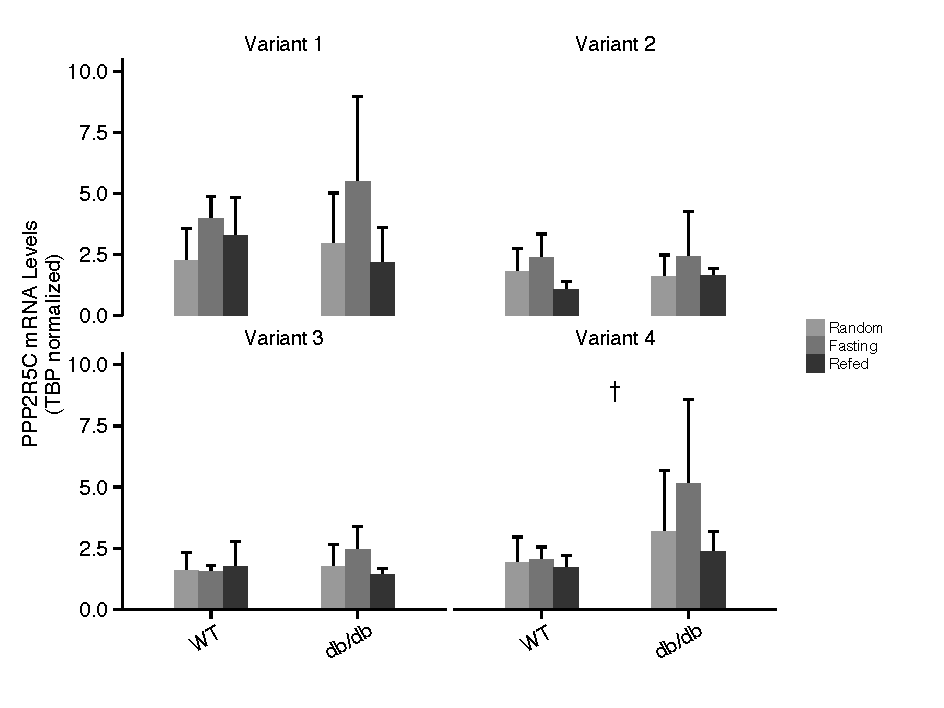
\includegraphics[width=1\textwidth]{figs/fig2-2 adipose ppp2r5c.pdf}
\caption[PPP2R5C expression in adipose tissues]{\footnotesize PPP2R5C is regulated in mouse adipose tissues. Mouse PPP2R5C transcript variant 1--4 mRNA levels in adipose tissues from 8-12 week C57BL/6 wild type or \textit{db/db} male mice under different nutritional statuses are shown here. Mice were fed with the normal chow diet without limit ("Random"). For "Fasting" and "Refed", mice were first starved for 16 hours and then allowed to the normal chow diet access for 6 hours. PPP2R5C Variant 1--4 are referenced according to NCBI. $\dagger$ for p-value<0.05 by \gls{ANOVA} analysis with comparison between wt and \textit{db/db} mice.}
\label{fig:fig2.2}
\end{figure}

In mouse abdominal white adipose tissues, there is also a significant trend in which most of \gls{ppp2r5c} variants have elevated mRNA levels in \textit{db/db} mice, especially for Variant 4 (Figure~\ref{fig:fig2.2}). There is a significant transcriptional increase in \textit{db/db} mouse adipose tissues in most nutritional statuses even with larger standard deviation compared with the liver \gls{ppp2r5c}. This phenomenon is also validated to be true in another independent qPCR analysis of mouse adipose samples, which was done by Katrin Stra{\ss}burger in our lab (data not shown). The same transcriptional change pattern shared between the liver and adipose tissue PPP2R5C indicates a similar function performed by PPP2R5C in the liver and adipose tissues. Interestingly, this match between adipose tissue and liver had also been reiterated in the liver and subcutaneous adipose tissues in healthy human controls and type 2 diabetic patients (See details in Section~\ref{sec:sec2.6}). This further indicates the conserved function of PPP2R5C between mice and human, and raises the interest to study PPP2R5C's role in metabolic diseases, such as Type 2 Diabetes. Combining the evolutionary similarity between adipose and liver (fat body in \textit{Drosophila} mimics the function of the liver and adipose tissues \cite{hietakangas_regulation_2009}), and the obese phenotype in PPP2R5C knockout mice and the fatty liver phenotype I have found after PPP2R5C knockdown in liver (Figure~\ref{fig:fig2.31}), it is reasonable to hypothesize the similar molecular function of PPP2R5C is shared by the mouse liver and adipose tissues. 

\begin{figure}[!tb]
\centering
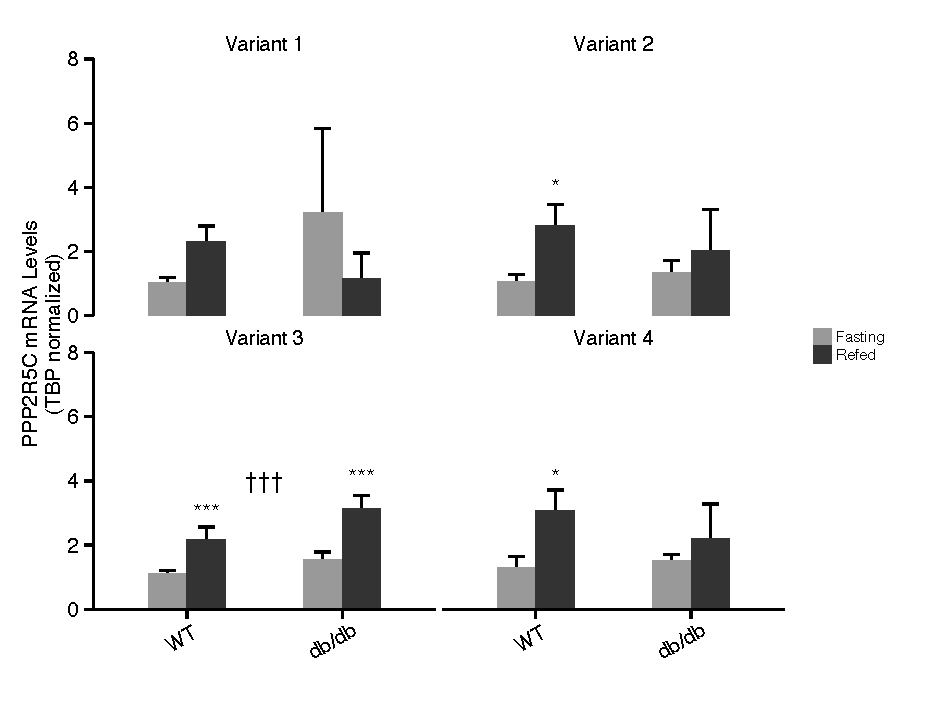
\includegraphics[width=1\textwidth]{figs/fig2-3 muscle ppp2r5c.pdf}
\caption[PPP2R5C expression in the muscle]{\footnotesize PPP2R5C is regulated in the mouse muscle. Mouse PPP2R5C transcript variant 1--4 mRNA levels in the muscle from 8-12 week C57BL/6 wildtype or \textit{db/db} male mice under different nutritional statuses are shown her. For "Fasting" and "Refed", mice were first starved for 16 hours and then allowed to the normal chow diet access for 6 hours. * and *** for p-value<0.05 and 0.001 by t-test within each mice genotype (WT or \textit{db/db}) and feeding regime (Random, Fasting, and Refed) in R. p-value was adjusted by Benjamini–Hochberg procedure in R. $\dagger\dagger\dagger$ for p-value<0.05 by \gls{ANOVA} analysis with comparison between wt and \textit{db/db} mice.}
\label{fig:fig2.3}
\end{figure}

PPP2R5C expression is nutritionally regulated in other metabolic relevant tissues such as the muscle, although in an opposite way as that for the liver and adipose tissues. In the mouse gastrocnemius muscle, PPP2R5C expression is increased upon re-feeding (Figure~\ref{fig:fig2.3}). This is significant for all variants except Variant 1, though the trend is still clear. However, this regulation is blunted in \textit{db/db}  mice compared to control mice in almost all isoforms but Variant 3. The Variant 3 in both wt and \textit{db/db} mice show an increased expression upon re-feeding. In addition, Variant 3 has also increased in \textit{db/db} mice. In comparison with the liver and adipose PPP2R5C, The opposite transcriptional response of PPP2R5C in the muscle during switch from fasting to re-feeding suggests a distinctive role of PPP2R5C in metabolically relevant tissues under different nutrient conditions.


\subsection{Transcriptional change of PPP2R5C in pathophysiology}

\begin{figure}[!tb]
\centering
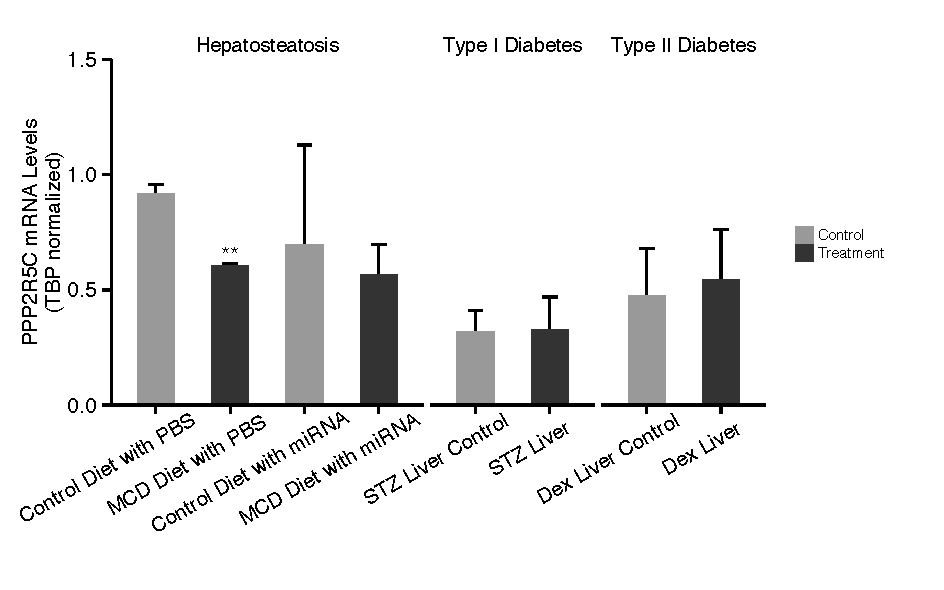
\includegraphics[width=1\textwidth]{figs/fig2-4 liver 34sample ppp2r5c.pdf}
\caption[PPP2R5C mRNA levels in Type I\&II Diabetes or Hepatosteatosis]{\footnotesize PPP2R5C transcriptional change in different pathophysiological conditions. Liver PPP2R5C mRNA levels were evaluated by qPCR in control or treatment group for the mouse model in Hepatosteatosis, Type I diabetes, and Type II diabetes. For Hepatosteatosis model, 16 week old male C57Bl6/J mice were fed with Methionine-Choline Deficient (MCD) diet or control diet for 4 weeks. In the Type I diabetes model, mice was treated with Streptozotocin (STZ) or control. For Type II diabetes model, mice was treated with Dexamethasone (Dex) or control. ** for p-value<0.01 by t-test in R.}
\label{fig:fig2.4}
\end{figure}

I have also tested PPP2R5C expression levels among various mouse models for different diseases such as Type I\&II diabetes and hepatosteatosis. The liver \gls{ppp2r5c} shows significantly reduced total mRNA level compared to control in the mouse liver from mouse hepatosteatosis model (Figure~\ref{fig:fig2.4}). However, in other disease models, there are no significant change in PPP2R5C mRNA level. In Dexamethasone induced mouse type 2 diabetes model, no strong increase in liver PPP2R5C mRNA levels shows a discrepancy with the genetic model of type 2 diabetes mouse model (\textit{db/db} in Figure~\ref{fig:fig2.1}). This difference could be due to different mechanisms for developing symptoms of type 2 diabetes in the mouse \cite{severino_low-dose_2002,king_use_2012}.  

In sum, although I have no data suggesting that these transcriptional changes have any functional relevance, these results suggest there might be links between \gls{ppp2r5c} and metabolic states or pathophysiological conditions. The transcription factor binding prediction \cite{_sabiosciences_????} on mouse PPP2R5C promoter shows several transcription factors, like \gls{nfkb} and HNF1\textalpha{}, are binding the mouse PPP2R5C promoter in ChIP assays. PPP2R5C has been shown to be involved in \gls{nfkb} pathway for T cell activation \cite{breuer_protein_2014}, and predicted \gls{nfkb} sites in PPP2R5C promoter indicate feedback regulation from \gls{nfkb} pathway. HNF1\textalpha{} has been genetically linked to maturity-onset diabetes of the young (MODY), and regulating several liver-specific gene expressions, such as albumin \cite{owen_monogenic_2013}. HNF1\textalpha{}'s potentially binding sites on PPP2R5C promoter indicate co-misregulation in diabetes.  

Although the whole body knockout mouse model for PPP2R5C showed increased adiposity \cite{varadkar_protein_2014}, distinct functions of PPP2R5C for metabolic homeostasis in a tissue-specific manner (in mammals) are widely unknown. A tissue-specific knockout or knockdown of PPP2R5C would shed more light on its functions in metabolic control. Since PPP2R5C has more than four splicing isoforms when the project was started, the primer sets 1--4 used throughout the thesis are representing more than one transcript of PPP2R5C (Figure~\ref{fig:fig2.0}). RNA sequencing for these samples would give more information about the differential regulation of various splicing isoforms.

\section{Antibody and virus preparation for PPP2R5C study}

\subsection{Selecting shRNA/miRNA for efficient knockdown of PPP2R5C}

In order to characterize the mammalian function of \gls{ppp2r5c},  I chose the mouse model  to decipher the molecular link for PPP2R5C in its potential role in metabolism. At the first step, I designed different \gls{shrna}s and \gls{mirna}s targeting common region of all PPP2R5C mRNA isoforms from online RNAi design website from Invitrogen \cite{_invitrogen_2014} (final candidates used throughout the thesis are shown in Figure~\ref{fig:fig2.0} and Table~\ref{tab:tab7}). Then I cloned shRNAs into pENTR U6, and miRNAs into pcDNA 6.2 GW EmGFP, both were purchased from Invitrogen. To have a reporter for PPP2R5C knockdown efficiency, I cloned PPP2R5C Variant 2 into 3\textsuperscript{$\prime$} UTR of renilla luciferase reporter (pRL-CMV renilla) and co-transfected with expression vectors for shRNAs and miRNAs in HEK293T cell. Knockdown efficiency was monitored for shRNAs and miRNAs as firefly luciferase normalized activity (Figure~\ref{fig:fig2.5}). 

\begin{figure}[htbp]
\centering
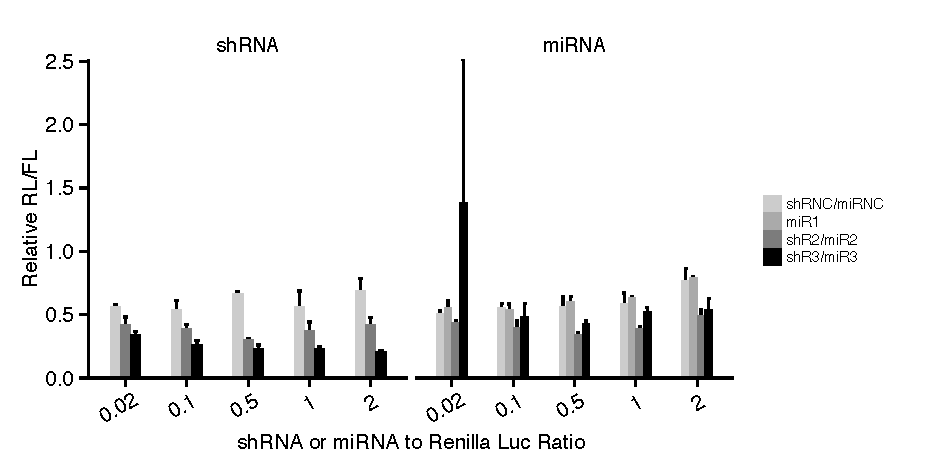
\includegraphics[width=1\textwidth]{figs/fig2-5 shR miR kd luc.pdf}
\caption[shRNA/miRNA KD efficiency on PPP2R5C luciferase reporter]{\footnotesize KD efficiency for shRNAs/miRNAs are measured on PPP2R5C variant 2 luciferase reporter. PPP2R5C variant 2 was cloned into 3\textsuperscript{$\prime$} UTR of firefly luciferase reporter (pRL-CMV renilla). RL-Var2 reporter was used to evaluated shRNA/miRNA KD efficiency via co-transfection with miRNA/shRNA expression construct at different ratios in HEK293T cell. Renilla luciferase (RL) activity was normalized against firefly luciferase (FL).}
\label{fig:fig2.5}
\end{figure}

After comparing the dynamic efficiency with different shRNAs or miRNAs to reporter plasmid ratios (Figure~\ref{fig:fig2.5}), shR3 is discovered to be the shRNA with strongest knockdown efficiency in all transfection settings with different ratios of shRNA expressing plasmid and PPP2R5C Variant 2 knockdown efficiency reporter. miR2 is the current best miRNA candidate while other two miRNAs have very mild knockdown efficiency. Furthermore, knockdown efficiency was also cross-validated by Western Blot of HA-tagged PPP2R5C Variant 2 (Figure~\ref{fig:fig2.6a}). Again, shR3 is shown to be the best shRNA candidate with almost complete knockdown at protein level when co-expressed with HA-tagged Variant 2. Thus, I chose shR3 to be the shRNA for PPP2R5C knockdown in different models, from cell to mouse. However, miRNA candidates have different performances in protein level knockdown (Figure~\ref{fig:fig2.6a}). miR3 has better knockdown efficiency than miR2 at protein level, but still has not reach the extent of shR3.

In order to achieve at least 80\% knockdown efficiency both in protein and transcription level, I did a bigger scale of searching \gls{mirna} candidate. I designed 12 new miRNAs and cloned them as before. I also performed similar Western Blot validation across various miRNAs (Figure~\ref{fig:fig2.6b}). In this experiment, miR12 was discovered to be the best miRNA against \gls{ppp2r5c} so far (only 5\% Variant 2 left comparing with control miRNA at protein level, Figure~\ref{fig:fig2.6c}), and chosen to be the miRNA for PPP2R5C knockdown \textit{in vivo}. 

\begin{figure}[htbp]
\centering

	\begin{subfigure}[t]{0.375\textwidth}
	\subcaption{shRNA/miRNA KD efficiency by western blot}
	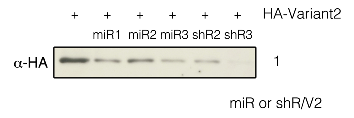
\includegraphics[width=1\textwidth]{figs/fig2-6a1.pdf}
    \label{fig:fig2.6a}
	\end{subfigure}%
          %add desired spacing between images, e. g. ~, \quad, \qquad, \hfill etc.
          %(or a blank line to force the subfigure onto a new line)
\\
	\begin{subfigure}[t]{0.625\textwidth}
	\subcaption{New set of miRNAs' KD efficiency by western blot}
	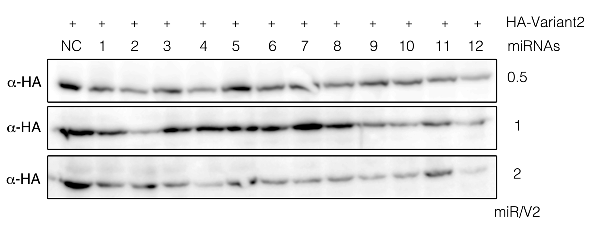
\includegraphics[width=1\textwidth]{figs/fig2-6a2.pdf}
    \label{fig:fig2.6b}
	\end{subfigure}%
          %add desired spacing between images, e. g. ~, \quad, \qquad, \hfill etc.
          %(or a blank line to force the subfigure onto a new line)
\\
	\begin{subfigure}[t]{1\textwidth}
	\subcaption{Quantification of miRNA's KD efficiency in (b)}
	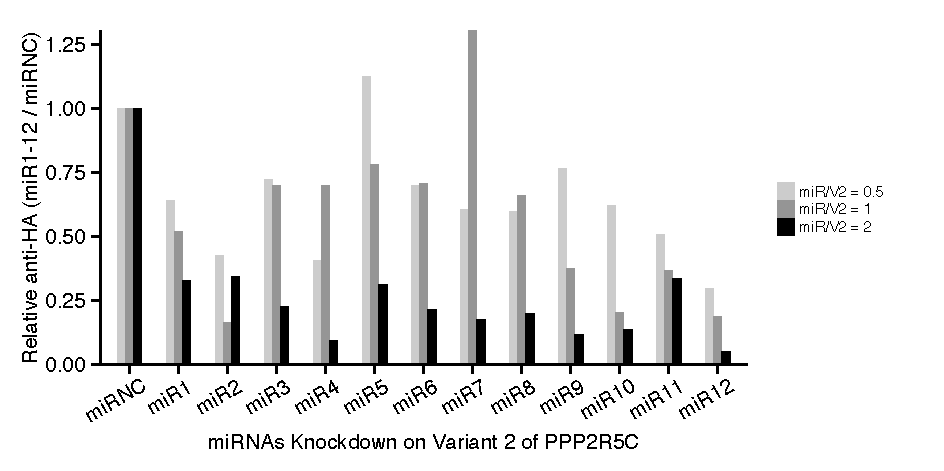
\includegraphics[width=1\textwidth]{figs/fig2-6b miR kd v2.pdf}
    \label{fig:fig2.6c}
	\end{subfigure}
\caption[shRNA/miRNA KD efficiency on PPP2R5C protein level]{\footnotesize Knockdown (KD) efficiency validated by western on PPP2R5C. (a--b) PPP2R5C KD efficiency by miRNAs and shRNAs. miRNA or shRNA construct was co-transfected with HA-tagged Variant 2 of PPP2R5C at different ratios in 293T cell. Total lysates after 3-day transfection were used to measure KD efficiency by blotting with \textalpha{}--HA antibody. (c) Quantification of miRNAs KD efficiency on PPP2R5C in Image J. }
\label{fig:fig2.6}
\end{figure}


\subsection{Generating Guinea Pig antibody for endogenous PPP2R5C detection}\label{sec:sec222}

To monitor \gls{ppp2r5c}'s endogenous regulation as well as the knockdown efficiency, I had to generate a specific antibody for mouse PPP2R5C. Although there was commercial antibody against mammalian PPP2R5C available from Abcam, I tested it and found it was failed in the specificity test, in which Variants 1--4 were over-expressed in mouse Hepa 1-6 cells to see any increased band matched with the size of PPP2R5C protein. Then I decided to make a polyclonal antibody against mouse PPP2R5C in the lab. I chose Variant 3 to be the immunizing antigen in guinea pig due to its smaller size, and potentially better solubility in bacteria than other isoforms. The recombinant Variant 3 was successfully produced in bacteria with a 6$\times$His tag. The IMAC (Immobilized metal ion Affinity Chromatography) purification gave a good amount enough for immunization (\textasciitilde1 mg). And the purity of recombinant Variant 3 was also good enough to have high specificity during antibody production (\textit{circa} 89\% in Coomassie brilliant blue staining, Figure~\ref{fig:fig2.7}). 

\begin{SCfigure} % side caption
\centering
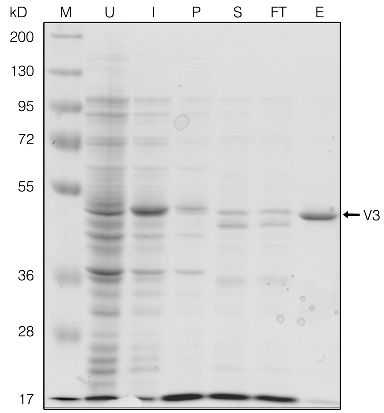
\includegraphics[width=0.5\textwidth]{figs/fig2-7 v3 purify.pdf}
\caption[Recombinant Variant 3 expression and purification]{\footnotesize PPP2R5C Variant 3 (V3) was cloned into pETM-11 (EMBL protein expression/purification facility) to be expressed in E. \textit{coli.} BL21-CodonPlus(DE3)-RIL strain. pETM-11 with V3 was electroporated into RIL and induced at 1 mM IPTG (Isopropyl \textbeta{}-D-1-thiogalactopyranoside) at 18 \celsius{} overnight. 1 mL bacteria before induction (U) and after induction (I) were taken to control the induction efficiency. Bacteria pellet after induction was lysed in lysis buffer (10mM MgCl\textsubscript{2}, 150mM NaCl, 10mM Imidazole, 20mM Tris pH 7.5) with 1 mg/ml Lysozyme, and separated into insoluble (P) and soluble fraction (S). Soluble fraction was loaded onto Ni-NTA column, and the flow-through fraction (FT) was collected. Final elute was collected in lysis buffer with 500mM Imidazole (E). All fractions from purification were run in 12\% SDS-PAGE gel with protein marker (M) and stained with GelCode Coomassie stain.}
\label{fig:fig2.7}
\end{SCfigure}

Polyclonal antibody production in guinea pig was produced with Freund's adjuvant. After 4th boosting immunization, I collected sera from guinea pig by heart puncture under animal welfare regulation in Germany, and with the generous help from Stefan F\"o{\ss}el in DKFZ's animal core facility. I tested the specificity of anti-sera for \gls{ppp2r5c} in both endogenous PPP2R5C knockdown (KD) and different PPP2R5C isoforms over-expression (Figure~\ref{fig:fig2.8}). Even at 1:5000 dilution, PPP2R5C anti-sera could still detect various PPP2R5C isoforms' over-expression and the endogenous knockdown of PPP2R5C by the adenovirus-packaged shR3 in Hepa 1-6.

\begin{figure}[htbp]
\centering
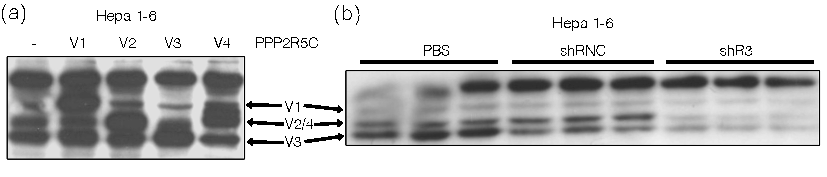
\includegraphics[width=1\textwidth]{figs/fig2-8 gp anti-v3 kd OE.pdf}
\caption[Specificity of GP antibody for PPP2R5C]{\footnotesize Antibody specificity for PPP2R5C in Hepa 1-6 lysates. (a) Variant 1--4 (V1--4) were over-expressed in Hepa 1-6 for 3 day. Total lysates from control (no over-expression) or V1--4 were submitted for Western Blotting by guinea pig antibody against PPP2R5C. V1--4 were corresponding to 3 lower bands. The most upper band could be non-specific band or other protein with high PPP2R5C homology, such as PPP2R5D. (b) knockdown efficiency on endogenous PPP2R5C by adenovirus packaged with shR3. 3 lower bands is size matched to V1--4 and showed a clear reduction in shR3. Band corresponding to V3 already showed reduction in shRNC comparing to PBS control.}
\label{fig:fig2.8}
\end{figure}

Interestingly, the adenovirus-packaged shRNC, which is a non-targeting scramble \gls{shrna}, strongly decreases the PPP2R5C protein level, especially for the band size-matched with Variant 3. And this is also true for the transcriptional level of \gls{ppp2r5c} (Figure~\ref{fig:fig2.9}). Specifically, Variant 3 mRNA level drops to around 40\% from low dosage (MOI (Multiplicity of Infection) = 10) to high dosage (MOI = 100, 200) of adenovirus infection. This indicates non-specific knockdown effect on Variant 3. It is known the adenovirus has strong immunogenic effect \cite{descamps_two_2009}. Strong immunogenicity could initiate some inflammation response which then affect the expression of PPP2R5C Variant 3. Interestingly, PPP2R5C has recently been shown to be involved in \gls{nfkb} mediated inflammation response \cite{breuer_protein_2014}. The PPP2R5C suppression upon high dose adenovirus infection suggests a feedback loop of PPP2R5C transcription in the immune response. This virus-mediated suppression of PPP2R5C could potentially controlled by \gls{nfkb} pathway on the predicted \gls{nfkb} sites in its promoter \cite{_sabiosciences_????}. 

\begin{figure}[htbp]
\centering
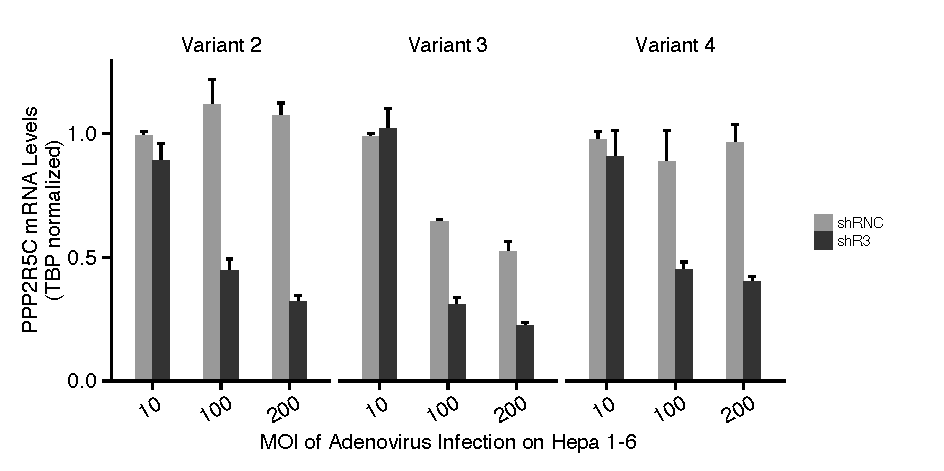
\includegraphics[width=1\textwidth]{figs/fig2-9 hepa ad kd.pdf}
\caption[Knockdown profile of endogenous PPP2R5C in Hepa 1-6]{\footnotesize Knockdown profile of endogenous PPP2R5C isoforms in Hepa 1-6 cells. Adenovirus with different \gls{moi}s (10, 100, 200) was diluted in PBS and infecting Hepa 1-6 for 3 days. The quantitative PCR analysis of PPP2R5C Variant 2/3/4 shows nice knockdown efficiency profile, which is dependent on MOI for all isoforms. MOI at 10 shows almost no reduction in mRNA level for all isoforms. MOI at 100 and 200 show a similar level of significant knockdown. Variant 3 is sensitive to control Adenovirus (shRNC) and shows a reduction in mRNA level at MOI of 100 or 200. }
\label{fig:fig2.9}
\end{figure}


\section{PPP2R5C negatively regulates glycolysis and lipogenesis}\label{sec:sec2.3}

\subsection{PPP2R5C KD in Hepa 1-6 increases glycolysis}

With efficient \textit{in vitro} knockdown tools for \gls{ppp2r5c}, I firstly studied the Hepa 1-6 to decipher the functional role of PPP2R5C, especially in metabolism control. As shown in Figure~\ref{fig:fig2.8}, endogenous PPP2R5C could be successfully knocked down at efficiency of 80\% by adenovirus-packaged shR3. After 3-day infection, mutant Hepa 1-6 cells with PPP2R5C knockdown show a clear increase in glycolysis, which is initially observed as deeper brownness of culture media in PPP2R5C KD Hepa 1-6 cells. Indeed, the glucose consumption assay (Figure~\ref{fig:fig2.10a}) indicates a strong increase in the glycolysis rate even in the last 24 hour of infection period. Accordingly, the lactate production (Figure~\ref{fig:fig2.10b}) has also similar extent of the increase as that in the glucose consumption. These pieces of evidence demonstrate that PPP2R5C could be a negative regulator of glycolysis.

\begin{figure}[htbp]
\centering
	\begin{subfigure}[t]{0.48\textwidth}
	\subcaption{Glucose consumption}
	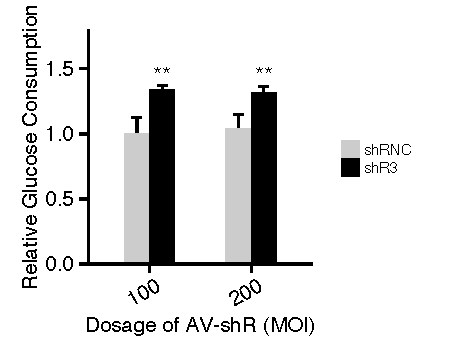
\includegraphics[width=1\textwidth]{figs/fig2-10a glucose kd.pdf}
    \label{fig:fig2.10a}
	\end{subfigure} %
~
	\begin{subfigure}[t]{0.48\textwidth}
	\subcaption{Lactate production}
	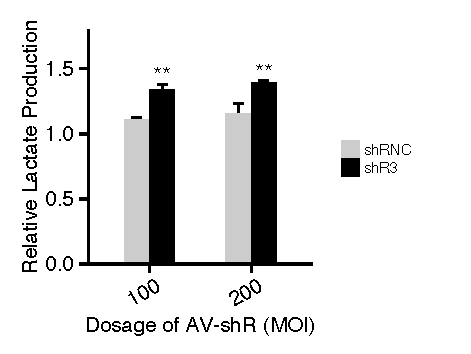
\includegraphics[width=1\textwidth]{figs/fig2-10b lactate kd.pdf}
    \label{fig:fig2.10b}
	\end{subfigure}
\caption[PPP2R5C KD increases glycolysis in Hepa 1-6]{\footnotesize PPP2R5C knockdown promotes the glucose consumption and lactate production in Hepa 1-6. Hepa 1-6 cells were infected with adenovirus packaged either with non-targeting scramble shRNA (shRNC) or PPP2R5C targeting (shR3) at \gls{moi} of 100 or 200 for 3-day knockdown. Infection was done in first 24 hours and then Hepa 1-6 cells were washed by fresh medium. The glucose consumption (a) and lactate production (b) were measured in the last 24-hour window of knockdown. They were background-subtracted from glucose and lactate concentration in fresh medium and normalized to total protein. ** for p-value<0.01 by t-test within each MOI in R.}
\label{fig:fig2.10}
\end{figure}

In addition, I also employed seahorse experiment to confirm the increased glycolysis phenotype after \gls{ppp2r5c} knockdown. When normalized to cell nuclei counting by DAPI staining, Hepa 1-6 knockdown cells have increased AUC (Area Under Curve) of glycolysis rate comparing with control adenovirus infected cells (Figure~\ref{fig:fig2.11}). The increase becomes statistically significant after oligomycin is added, which boosts the maximal glycolytic activity. Combining with data from glucose consumption and lactate production (Figure~\ref{fig:fig2.10}), it is clearly demonstrated that the PPP2R5C knockdown promotes the glucose uptake and glycolysis in Hepa 1-6 cells.

\begin{figure}[htbp]
\centering
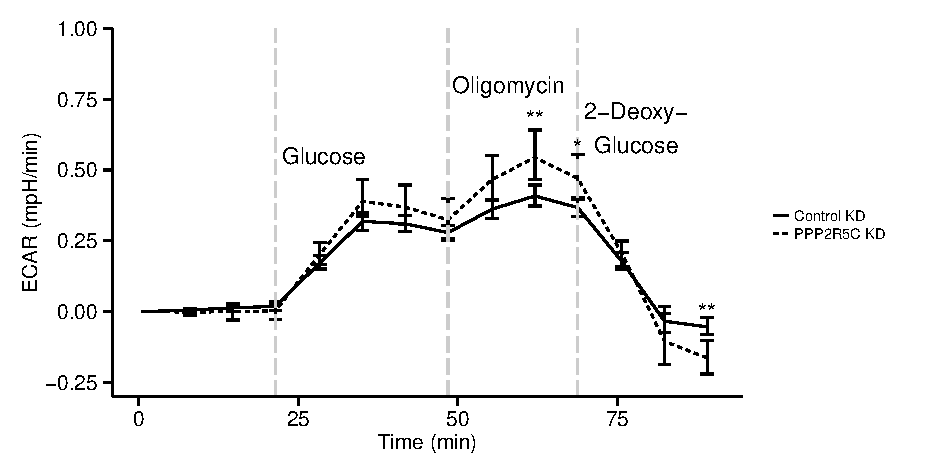
\includegraphics[width=1\textwidth]{figs/fig2-11 seahorse.pdf}
\caption[PPP2R5C KD promotes glycolysis by seahorse measurement]{\footnotesize PPP2R5C Knockdown promotes glycolysis in seahorse experiment. Adenovirus with MOI=100 was diluted in PBS and infected Hepa 1-6 for 2 days. Then infected Hepa 1-6 was digested with trypsin from the culture plate and re-plated in 96-well plate with balanced cell number between different groups (Control KD for shRNC, and PPP2R5C KD for shR3). Glycolysis activity was measured on seahorse instrument with glycolysis stress kit. Glucose, oligomycin and 2-Deoxy-Glucose were added at the time of vertical dashed line according to the protocol in the kit. The extracellular acidification rate (ECAR, mpH/min) was recorded as an indirect readout for intracellular glycolysis rate. * and ** for p-value<0.05 and 0.01 by Wilcoxon signed-rank test.}
\label{fig:fig2.11}
\end{figure}

\subsection{PPP2R5C KD promotes glucose uptake rate in Hepa 1-6}

Although \gls{ppp2r5c} is shown to be a negative regulator of glycolysis, it is still not clear the increased glucose consumption is due to increased cell number with the same glucose uptake rate or increased glucose uptake rate within the same number of cells. On one hand, the total protein content after PPP2R5C knockdown has not changed between control and PPP2R5C knockdown cells (data not shown), which indicates no strong increase in cell proliferation. On other hand, I employed a short-term glucose uptake assay to assess the glucose uptake activity of Hepa 1-6 by measuring \gls{2nbdg} uptake in 20 min via \gls{facs} (\cref{fig:fig2.12,fig:fig2.13,fig:fig2.14}), in order to eliminate any glucose uptake effect from increasing cell number during assay time in Figure~\ref{fig:fig2.10a}. 2NBDG is a fluorescent 2-deoxyglucose analog which was widely used to monitor glucose uptake rate \cite{zou_2-nbdg_2005,nitin_molecular_2009,oneil_uptake_2005,zhong_histone_2010,kawauchi_p53_2008}.

\begin{figure}[!tbp]
\centering
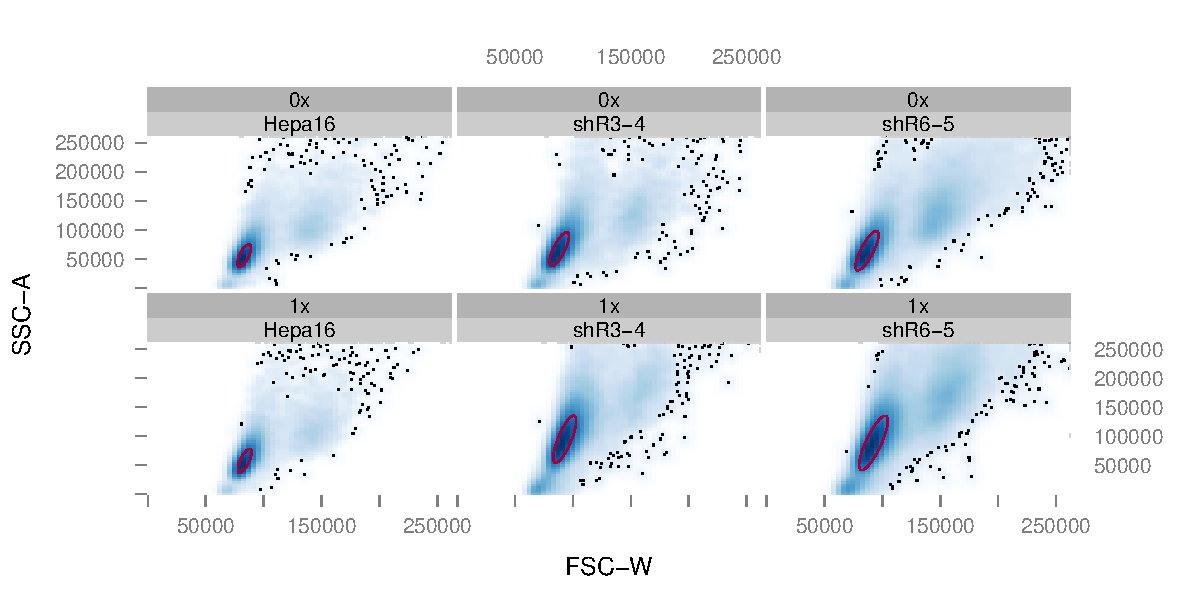
\includegraphics[width=1\textwidth]{figs/fig2-12 facs filter.pdf}
\caption[FACS filtering for single live Hepa 1-6 cell]{\footnotesize Single live Hepa 1-6 cell filtering in FACS by R. X-coordinate is marker for cell size (FSC-W, \textbf{F}oward-\textbf{S}cattered \textbf{W}idth), and y-coordinate is cell granularity (SSC-A, \textbf{S}ide-\textbf{S}cattered \textbf{A}rea). Hepa 1-6 with stable shRNAs (shR3 or shR6) or not were induced at 30 $\mu$g/mL cumate (1x, 0x for DMSO control) for 3 day and then starved in serum-free DMEM overnight. shR3-4 and shR6-5 were single clone for shR3 and shR6. Then these cells were sensitized in KRPH (Krebs-Ringer-Phosphate-HEPES) buffer for 1 hour and followed by 20 min incubation with 100 $\mu$M 2NBDG. Finally, Hepa 1-6 cells were digested with trypsin for 3 minutes and subjected to FACS analysis. Single live Hepa 1-6 cells were clustered in FSC-SSC scatter plot and filtered out in R by using package flowCore (indicated by red circle on scatter plot).}
\label{fig:fig2.12}
\end{figure}

\begin{SCfigure}
\centering
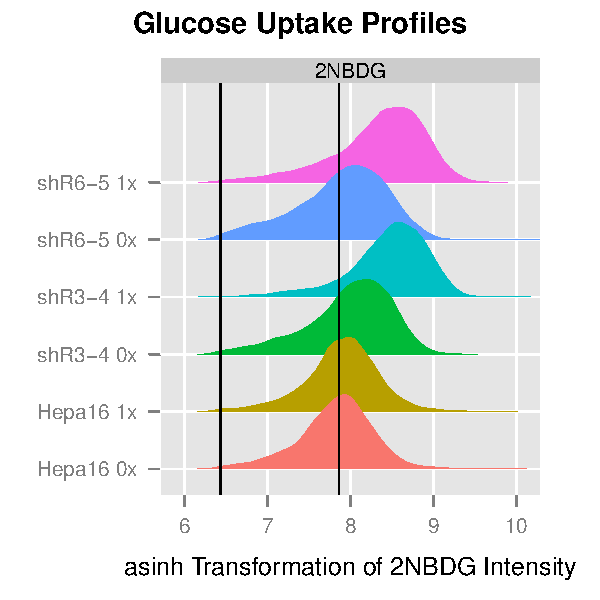
\includegraphics[width=0.5\textwidth]{figs/fig2-13 density 2NBDG.pdf}
\caption[Density plot of 2NBDG+ Hepa 1-6]{\footnotesize Density plot of Hepa 1-6 cell with positive 2NBDG uptake. Filtered single live Hepa 1-6 cells were compared for 2NBDG fluorescence intensity between Hepa 1-6 cell with 2NBDG incubation and the one without 2NBDG incubation to calculate a threshold for 2NBDG uptake (left vertical line). Median intensity in Hepa 1-6 without cumate induction (right vertical line) was calculated for better comparison between different cell lines. shR3-4 and shR6-5 were single clone for shR3 and shR6. 0x and 1x were DMSO control and 30 $\mu$g/mL cumate induction for 3 days. The fluorescence intensity was \textit{asinh} transformed to have a nice representation of intensity at different magnitudes.}
\label{fig:fig2.13}
\end{SCfigure}

Additionally, I cloned 2 sets of \gls{shrna}s (shR3 and shR6)  into a miR30-based inducible shRNA expression vector \cite{fellmann_functional_2011,_piggybac_????}, and stable Hepa 1-6 cell lines harboring genome-integrated inducible shR3 or shR6 were generated after puromycin selection. The stable inducible cell lines were used as cross-validation for results from the adenovirus-packaged shR3, and supposed to eliminate any potential virus-mediated effects given the fact of high immunogenicity of adenovirus and non-specific down-regulation on Variant 3 of PPP2R5C by adenovirus. The shR3 and shR6 expression were induced by 30$\mu$g/mL cumate for 3--4 days to achieve similar extent of knockdown efficiency as that in the adenovirus packaged shR3.

I analyzed all the data from FACS either in flowCore \cite{ellis_flowcore:_????}, flowStats \cite{hahne_flowstats:_????} and flowViz \cite{ellis_flowviz:_????} package in R, and validated the analysis again in FlowJo. There are mainly two populations in all cell lines  based on the size distribution (from empty Hepa 1-6 to two stable inducible \gls{shrna} cell lines) (Figure~\ref{fig:fig2.12}). And these two populations have not changed after shRNA expression by induction with 30 $\mu$g/mL cumate, which indicates no significant cell morphological change after \gls{ppp2r5c} knockdown. Based on particle size (FSC), it is clear that the population at the left is single live cells, and the population on the right is doublet Hepa 1-6 cells potentially from incomplete digestion by trypsin. For accurate single cell glucose uptake measurement, I chose the single live cell population for glucose uptake assay by FACS.

\begin{figure}[htbp]
\centering
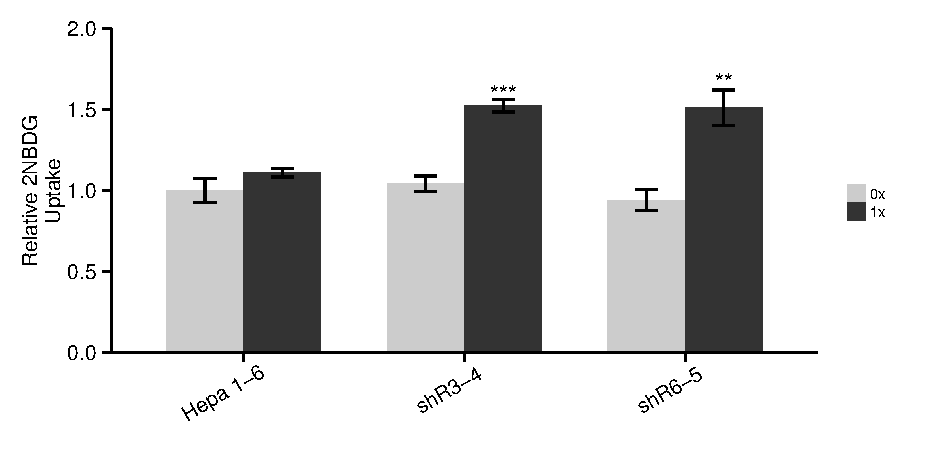
\includegraphics[width=1\textwidth]{figs/fig2-14 facs glucose uptake.pdf}
\caption[Relative quantification of 2NBDG uptake upon PPP2R5C KD]{\footnotesize 2NBDG uptake in Hepa 1-6 upon PPP2R5C knockdown. FACS data for 2NBDG uptake in empty Hepa 1-6, Hepa 1-6 with inducible shR3 and 6 (single clone shR3-4 and shR6-5) were induced at DMSO (0x) or 30 $\mu$g/mL cumate (1x) and analyzed as described in Figure~\ref{fig:fig2.13} and Figure~\ref{fig:fig2.12}. ** and *** for p-value<0.01 and 0.001 by t-test in R. }
\label{fig:fig2.14}
\end{figure}

In the first step, single live Hepa 1-6 cells were filtered out based on size (red circled area in Figure~\ref{fig:fig2.12}) with a 2D-normal distributed contour from flowCore package. Then, single live Hepa 1-6 cells were analyzed to calculate the proportion of 2NBDG positive staining with 2NBDG un-stained Hepa 1-6 cells as negative staining control. From the \textit{asinh} transformed density map of all 2NBDG positive staining, there is a obvious red-shift in the density map after \gls{ppp2r5c} knockdown (Figure~\ref{fig:fig2.13}), and almost all single live Hepa 1-6 cells have positive 2NBDG uptake. For empty Hepa 1-6 cells, there is no red-shift in density map after the cumate induction. These data clearly show that PPP2R5C knockdown could increase glucose uptake even in very short time period, such as 20 minutes. The quantification of median fluorescence intensity (MFI) is normalized and showed in Figure~\ref{fig:fig2.14}. The same phenotype has also been observed in a third independent shRNA for PPP2R5C (shR8, data not shown). 

\begin{figure}[htbp]
\centering
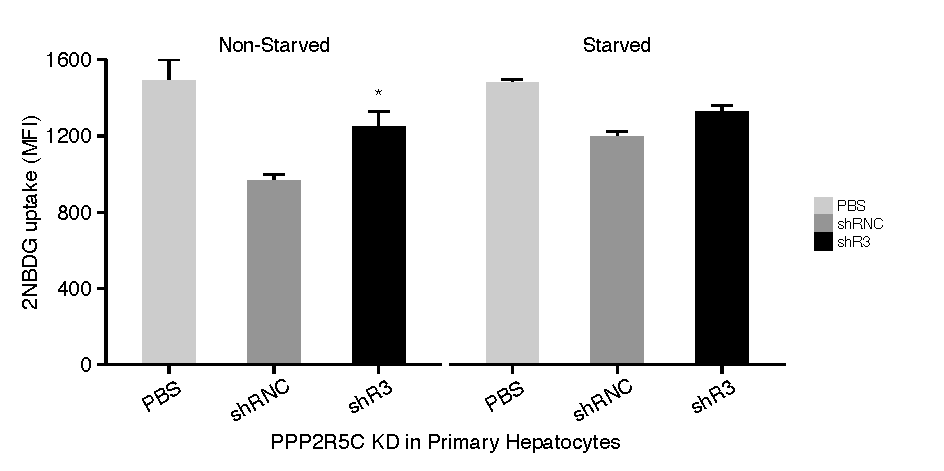
\includegraphics[width=1\textwidth]{figs/fig2-15 1st hepa glucose uptake facs.pdf}
\caption[2NBDG uptake in primary hepatocytes]{\footnotesize 2NBDG uptake in mouse primary hepatocytes upon PPP2R5C knockdown by the adenovirus with shRNC or shR3. FACS data were collected and analyzed as described in Figure~\ref{fig:fig2.14}. * for p-value<0.05 by t-test in R. n=3.}
\label{fig:fig2.15}
\end{figure}

In mouse primary hepatocytes, there is also a nice cross-validation of glucose uptake phenotype observed in Hepa 1-6 cells (Figure~\ref{fig:fig2.15}). At two different nutritional statuses, either starved for serum or non-starved, the glucose uptake, which is determined by FACS measurement of 2NBDG uptake as that in Figure~\ref{fig:fig2.14}, shows clear trend of increase in \gls{ppp2r5c} knockdown cells comparing with non-targeting \gls{shrna} control cells. For non-starved condition, the increase is statistically significant. Again, the non-targeting shRNA control adenovirus still has some non-specific virus effect on glucose uptake comparing with PBS control.

\subsection{PPP2R5C deficiency promotes \textit{de novo} lipogenesis}

Another interesting phenotype by \gls{ppp2r5c} knockdown is the increased lipid storage in the cultured primary hepatocytes (Figure~\ref{fig:fig2.16}). For cultivated mouse primary hepatocytes, I have received two sources of them, from Prof. Herzig's and Prof. Klingm\"uller's lab especially. These two sources of hepatocytes were prepared in their corresponding lab with the same protocol of isolation. However, hepatocytes from Prof. Klingm\"uller's lab were additionally counted for living cell by trypan blue staining. With these two different sources of mouse primary hepatocytes, the PPP2R5C knockdown via adenovirus-packaged shR3 shows a significant increase (approximately 2-fold) in the triglyceride storage comparing to the non-targeting shRNC or PBS control. Although relative extent of lipid storage increase is proportionally augmented with the duration of knockdown, prolonged \textit{in vitro} cultivation of primary hepatocytes sometimes ended up with de-differentiation of the hepatocyte. The de-differentiated primary hepatocytes usually show distorted and shrunken cell shape. The lipid storage increase phenotype could not be observed under this condition, such as 3-day adenovirus infected hepatocytes from Prof. Herzig's Lab at DKFZ ("Herzig 3 Day" in Figure~\ref{fig:fig2.16}). 

\begin{figure}[htbp]
\centering
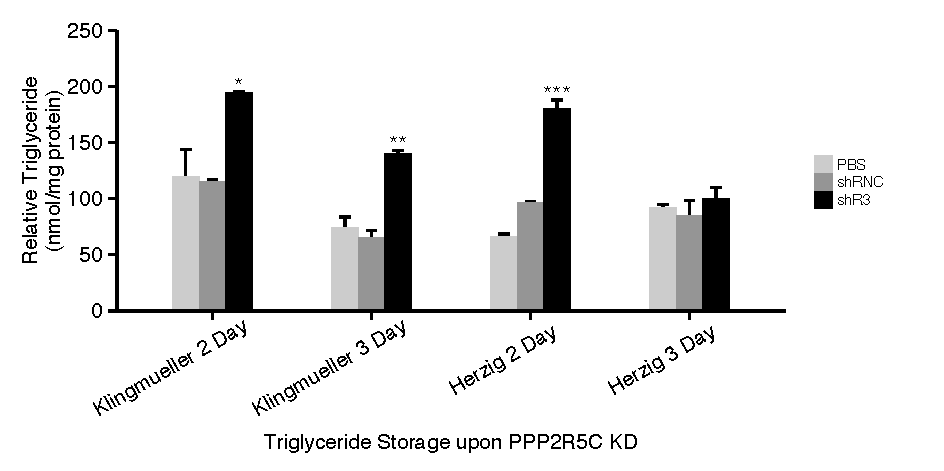
\includegraphics[width=1\textwidth]{figs/fig2-16 1st hepa tag.pdf}
\caption[Triglyceride in primary hepatocytes upon PPP2R5C KD]{\footnotesize PPP2R5C knockdown increases lipid storage in primary hepatocytes. Primary hepatocytes were infected with adenovirus at the same condition as in Figure~\ref{fig:fig2.15}. Lipid fraction was extracted by methanol-chloroform method \cite{folch_simple_1957} and measured for free glycerol released from lipase digestion.  *, ** and *** for p-value<0.05, 0.01 and 0.001 by t-test in R, n=3.}
\label{fig:fig2.16}
\end{figure}

In contrary to the shRNC effect on glycolysis phenotype, the non-targeting scramble \gls{shrna} showed no effect on the lipid storage when that was comparing with PBS control. This discrepancy possibly implied complex and different mechanisms in changing glycolysis and lipid storage after \gls{ppp2r5c} knockdown. 

\begin{figure}[htbp]
\centering
	\begin{subfigure}[t]{0.48\textwidth}
	\subcaption{ATP Level}
	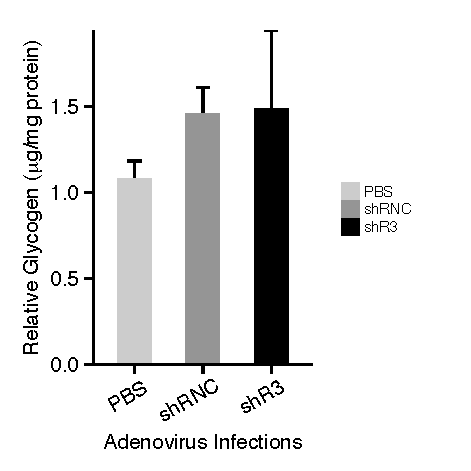
\includegraphics[width=1\textwidth]{figs/fig2-17a 1st hepa glycogen.pdf}
    \label{fig:fig2.17a}
	\end{subfigure} %
~
	\begin{subfigure}[t]{0.48\textwidth}
	\subcaption{Glycogen Storage}
	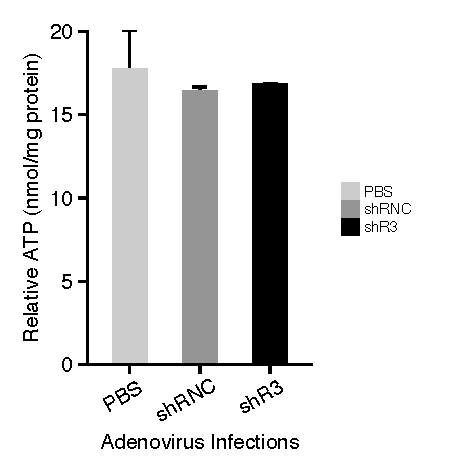
\includegraphics[width=1\textwidth]{figs/fig2-17b 1st hepa atp.pdf}
    \label{fig:fig2.17b}
	\end{subfigure}
\caption[PPP2R5C KD has no effect on ATP and Glycogen in 1\textsuperscript{o} Hepatocytes]{\footnotesize PPP2R5C knockdown does not change the ATP level (a) or the glycogen storage (b) in mouse primary hepatocytes. Primary hepatocytes were infected with the adenovirus at the same condition as in Figure~\ref{fig:fig2.14}. n=3.}
\label{fig:fig2.17}
\end{figure}

In addition to the lipid storage and glycolysis phenotype, the PPP2R5C knockdown in primary hepatocyte has no effect on the \gls{ATP} level (Figure~\ref{fig:fig2.17a}) and glycogen level (Figure~\ref{fig:fig2.17b}). This indicates the excessive energy from the increased glucose uptake is shunted into the energy storage as triglyceride storage, but not as the \gls{ATP} or glycogen in cultivated primary hepatocytes. 

\begin{figure}[htbp]
\centering
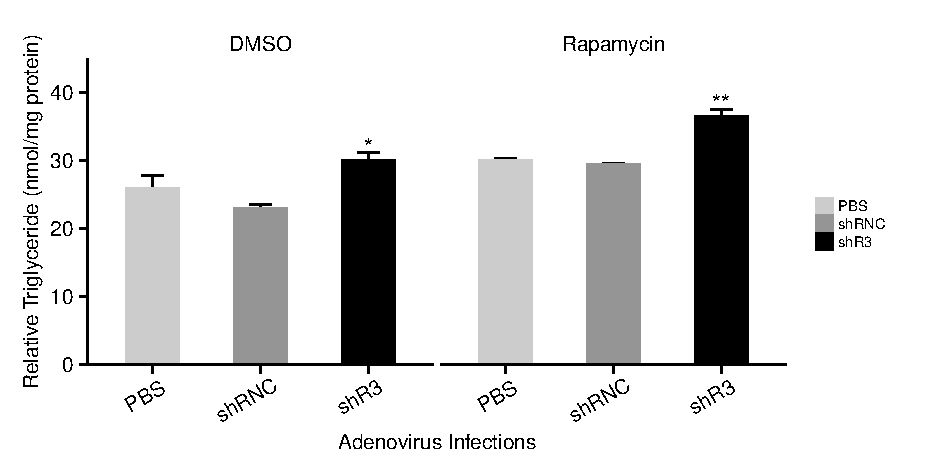
\includegraphics[width=1\textwidth]{figs/fig2-18 hepa tag rapamycin.pdf}
\caption[Triglyceride increases in Hepa 1-6 upon PPP2R5C KD]{\footnotesize PPP2R5C knockdown increases lipid storage in Hepa 1-6 independently of mTOR. Hepa 1-6 were infected with adenovirus at the same condition as in Figure~\ref{fig:fig2.10}. Lipid fraction was extracted by methanol-chloroform method and measured for free glycerol released from lipase digestion.  *, ** for p-value<0.05, 0.01 by t-test in R, n=3.}
\label{fig:fig2.18}
\end{figure}

Moreover, the lipid storage phenotype in \gls{ppp2r5c} knockdown is also conserved in another cell type, Hepa 1-6 cells (Figure~\ref{fig:fig2.18}). Even treated with \gls{mtor} inhibitor rapamycin, the lipid storage phenotype is still present without compromising its increase. This evidence indicates the mechanism how PPP2R5C affect lipid storage is either at the downstream of \gls{mtor} or in parallel with \gls{mtor}. It has been shown that the mTORC1 activation leads to the increase in glycolysis and lipogenesis via the  downstream activation of HIF1\textalpha{} and SREBP-1 \cite{duvel_activation_2010}. The increased glycolysis and lipogenesis in PPP2R5C knockdown is a phenocopy for the mTORC1 activation. 

\begin{figure}[!tb]
\centering
	\begin{subfigure}[t]{0.48\textwidth}
	\subcaption{Free Fatty Acid Uptake}
	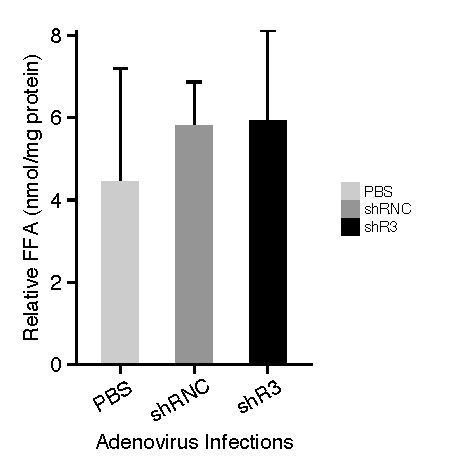
\includegraphics[width=1\textwidth]{figs/fig2-19a hepa ffa uptake.pdf}
    \label{fig:fig2.19a}
	\end{subfigure} %
~
	\begin{subfigure}[t]{0.48\textwidth}
	\subcaption{Intracellular Steady-state Free Fatty Acid}
	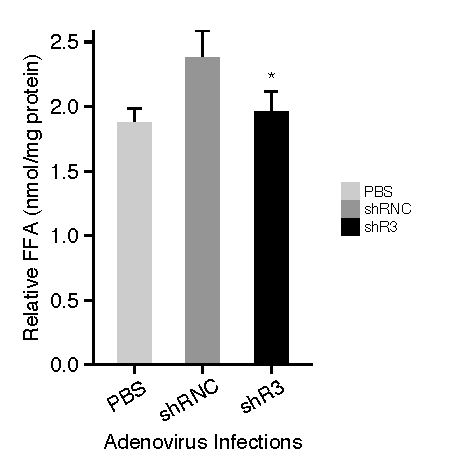
\includegraphics[width=1\textwidth]{figs/fig2-19b hepa ffa intracellular.pdf}
    \label{fig:fig2.19b}
	\end{subfigure}
\caption[Free Fatty Acid uptake is not responsible for increased triglyceride]{\footnotesize Free fatty acid in culture medium is not responsible for increased triglyceride storage inside Hepa 1-6. (a) Free fatty acid from culture media was enriched by methanol-chloroform method \cite{folch_simple_1957} and uptake was calculated from the difference in free fatty acid between fresh medium and medium after 3-day culturing. (b) Intracellular free fatty acid level. Hepa 1-6 cells were infected with adenovirus at the same condition as in Figure~\ref{fig:fig2.14}. * for p-value<0.05 by t-test in R, n=3.}
\label{fig:fig2.19}
\end{figure}

In order to further clarify the lipid storage phenotype is a result of the increased \textit{de novo} lipogenesis but not the re-esterification of absorbed free fatty acids, I measured the free fatty acid uptake from culture media and the intracellular free fatty acid in Hepa 1-6 cells upon \gls{ppp2r5c} knockdown (Figure~\ref{fig:fig2.19}). Neither of them is increased after PPP2R5C knockdown. No increase in free fatty acid uptake suggests the accumulated lipid storage could come from \textit{de novo} lipogenesis. If comparing the relative concentration of free fatty acid uptake during 3-day infection with that for fatty acid equivalent increment in triglyceride after PPP2R5C knockdown (approximately comparing 6 nmol/(mg protein) with 30 nmol/(mg protein), 1 molecule of triglyceride consists of 3 molecules of fatty acid), it is very unlikely that the increased triglyceride storage phenotype comes from the increased re-esterification of absorbed free fatty acids, but rather from \textit{de novo} biosynthesis. Also, the slight decrease in the intracellular free fatty acid concentration after PPP2R5C implies a higher flux from intracellular free fatty acid toward triglyceride synthesis when comparing with shRNC.


\section{PPP2R5C \textit{in vivo} knockdown promotes glucose uptake, triglyceride synthesis}

It was interesting to know the \gls{ppp2r5c}'s role in a cellular model, such as the Hepa 1-6 or mouse primary hepatocyte (Section~\ref{sec:sec2.3}). Data in cell culture suggested PPP2R5C's potential role in metabolism is shunting the absorbed glucose into lipid storage in a cell-autonomous fashion. But it was always more physiological-relevant when investigating the PPP2R5C's function in metabolism \textit{in vivo}. To achieve this purpose, I employed adeno-associated virus (AAV) to specifically express the \gls{mirna} targeting PPP2R5C (miR12, see Figure~\ref{fig:fig2.0} and Table~\ref{tab:tab7}) in the mouse liver and perform a long-term knockdown \textit{in vivo} as described \cite{kulozik_hepatic_2011}. Previously, the miR12 was selected as miRNA candidate based on its highest efficiency in knockdown tested in HEK293T cell (Figure~\ref{fig:fig2.6c}). The \gls{AAV} packaged miR12 was produced from Vector Biolabs (Philadelphia, USA) due to the  insufficient in-house virus production yield. I performed a pilot mouse experiment  to evaluate the \textit{in vivo} knockdown efficiency in the mouse liver. From the qPCR analysis of total PPP2R5C mRNA (Figure~\ref{fig:fig2.20a}) and protein level (Figure~\ref{fig:fig2.20b}), there is a strong reduction in both transcriptional and protein level. This AAV packaged miR12 gave me the appropriate tool to have a liver-specific manipulation of the mouse PPP2R5C. 

\begin{figure}[htbp]
\centering
	\begin{subfigure}[t]{0.48\textwidth}
	\subcaption{Knockdown efficiency by qPCR}
	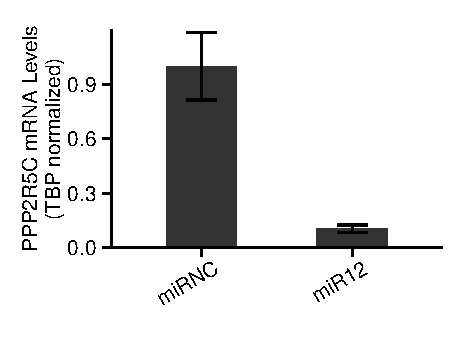
\includegraphics[width=1\textwidth]{figs/fig2-20a pilot qPCR.pdf}
    \label{fig:fig2.20a}
	\end{subfigure} %
~
	\begin{subfigure}[t]{0.48\textwidth}
	\subcaption{Knockdown efficiency in protein level}
	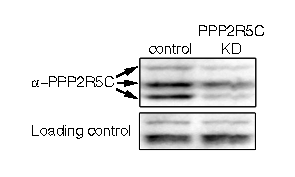
\includegraphics[width=1\textwidth]{figs/fig2-20b kd in vivo protein.pdf}
    \label{fig:fig2.20b}
	\end{subfigure}
\caption[KD efficiency for miR12 \textit{in vivo}]{\footnotesize PPP2R5C knockdown efficiency in vivo. (a) miR12's \textit{in vivo} knockdown efficiency was compared with the non-targeting control miRNC after 2 week AAV injection. qPCR was performed with the probe set for total mRNA of PPP2R5C in the liver. (b) Knockdown efficiency was evaluated at protein level. The liver endogenous PPP2R5C was detected by the home-made guinea pig antibody against it. Non-specific binding band was showed at bottom as the loading control. n=5 for qPCR analysis.}
\label{fig:fig2.20}
\end{figure}

\subsection{PPP2R5C knockdown has no impact on animal health}

With the knowledge of miR12's \textit{in vivo} knockdown efficiency, I performed another mouse experiment with longer AAV infection in order to see the relatively long term effect of PPP2R5C in metabolism. With 7 weeks of \gls{ppp2r5c} knockdown in the mouse liver, there is no severe side effect from \gls{AAV} infection, which could be demonstrated by the low level of serum \gls{alt} level and no further increase in knockdown mice (Figure~\ref{fig:fig2.21}). ALT is an enzyme mainly expressed in the liver, much less expressed in kidney, heart, muscle. The serum ALT level is normally low, and only become high when the liver is damaged or diseased (leakage across damaged hepatic cell membrane). Serum ALT level around 20 U/L was much lower than that from mice suffering liver injury (several hundred to even thunsands U/L \cite{masaki_role_2005}). 

\begin{figure}[htbp]
\centering
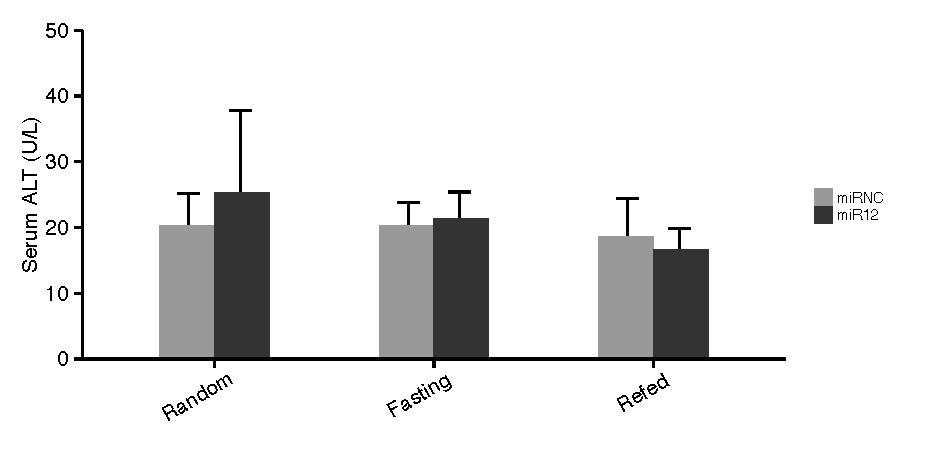
\includegraphics[width=1\textwidth]{figs/fig2-21 serum ALT.pdf}
\caption[Serum ALT after PPP2R5C KD]{\footnotesize Serum ALT (Alanine Aminotransferase) level indicates no liver injury. 8-10 week CL57BL/6 male mice were injected with adeno-associated virus packaged \gls{mirna} against mouse PPP2R5C (miR12) or scramble miRNA (miRNC) at 1$\times$10\textsuperscript{11} viral particles/mouse via tail injection in 100 $\mu$L PBS. And injected mice was sacrificed after 7-week knockdown. Before sacrificing, mice were divided into different groups for various treatments, including \textit{ad libitum} fed (Random), 16 hour fasting (Fasting), and 16 hour fasting followed by 6 hour feeding (Refed). 5 $\mu$L serum was used to measure ALT enzymatic activity. n=5 or 6.}
\label{fig:fig2.21}
\end{figure}

During the \gls{AAV} infection, mice from control and knockdown group (miRNC vs miR12) have also no significant difference in the body weight growing profile (Figure~\ref{fig:fig2.22}), which indicates no strong whole body growth change after the liver-specific PPP2R5C KD. Furthermore, I have also performed the body composition analysis  in these mice every 2 or 3 week by using echoMRI measurement. There is also no significant difference in fat (Figure~\ref{fig:fig2.22}) and lean mass (data not shown) profile between control and knockdown group. Although these mice subjected into fasting before final preparation show some difference before virus injection, and the difference remained constant during knockdown and contributed to the overall baseline difference in control and knockdown group. After sacrificing, I also measured the mouse abdominal white adipose tissue weight (Figure~\ref{fig:fig2.25}). There is also no change in abdominal white adipose tissue weight upon PPP2R5C KD. In summary, 7-week liver-specific PPP2R5C knockdown via \gls{AAV} infection has no significant morphological changes to the size of tissues or to the whole body.

\begin{figure}[htbp]
\centering
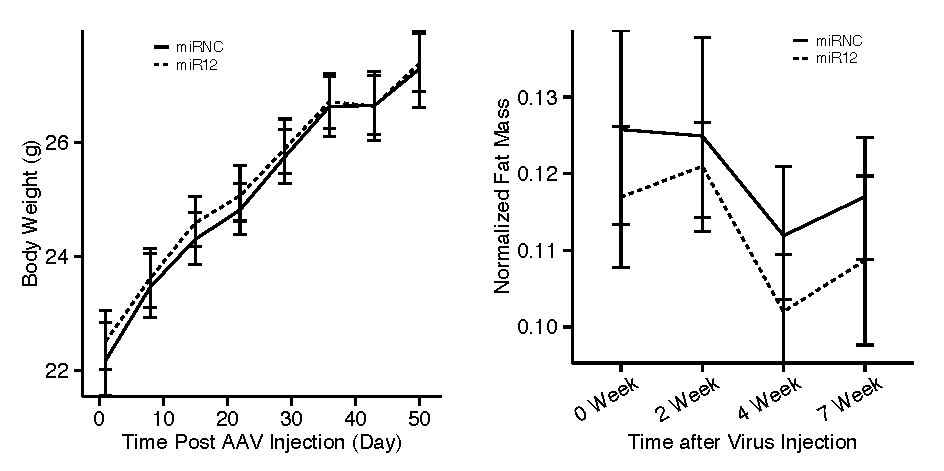
\includegraphics[width=1\textwidth]{figs/fig2-22 body weight and echoMRI fat.pdf}
\caption[Body weight and fat composition change after PPP2R5C KD]{\footnotesize Body weight and fat composition profile have no change after PPP2R5C knockdown. Mice in Figure~\ref{fig:fig2.21} were measured for body weight at each week (left panel). Time 0 was the body weight before virus injection. Whole body fat composition was calculated from fat content normalized to body weight at each time point (right panel). Week 0 indicated fat composition before virus injection. n=5 or 6.}
\label{fig:fig2.22}
\end{figure}

%\begin{figure}[htbp]
%\centering
%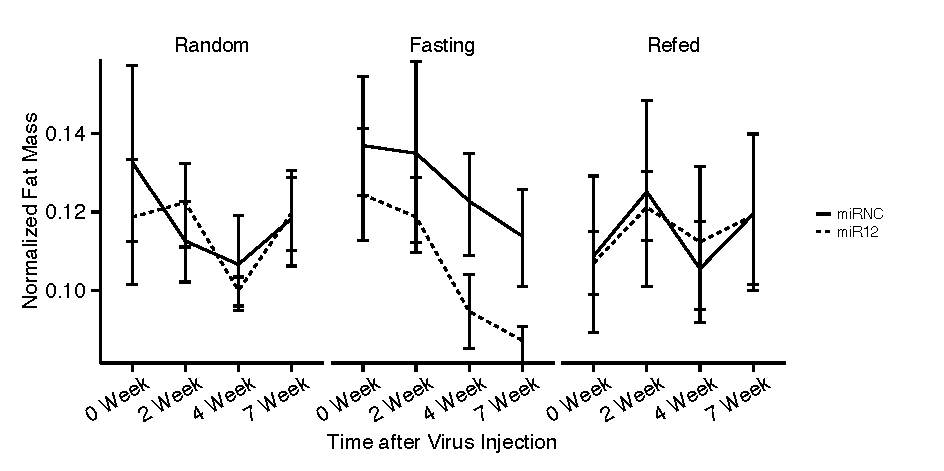
\includegraphics[width=1\textwidth]{figs/fig2-23 echoMRI fat.pdf}
%\caption[Body fat content profile after PPP2R5C KD]{\footnotesize Body fat content profile has no change after PPP2R5C knockdown. Mice were the same as Figure~\ref{fig:fig2.21}. Whole body fat composition was calculated from fat content normalized to body weight at each time point. Week 0 indicated fat composition before virus injection. n=5 or 6}
%\label{fig:fig2.23}
%\end{figure}

%\begin{figure}[htbp]
%\centering
%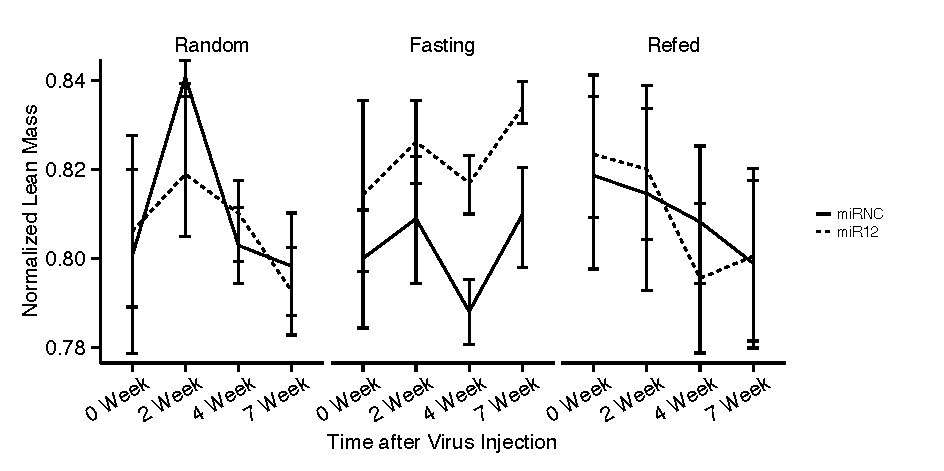
\includegraphics[width=1\textwidth]{figs/fig2-24 echoMRI lean.pdf}
%\caption[Body lean mass profile after PPP2R5C KD]{\footnotesize Body lean mass profile has no change after PPP2R5C knockdown. Mice were the same as Figure~\ref{fig:fig2.21}. Whole body lean mass composition was calculated from lean mass content normalized to body weight at each time point. Week 0 indicated fat composition before virus injection. n=5 or 6}
%\label{fig:fig2.24}
%\end{figure}

\begin{figure}[htbp]
\centering
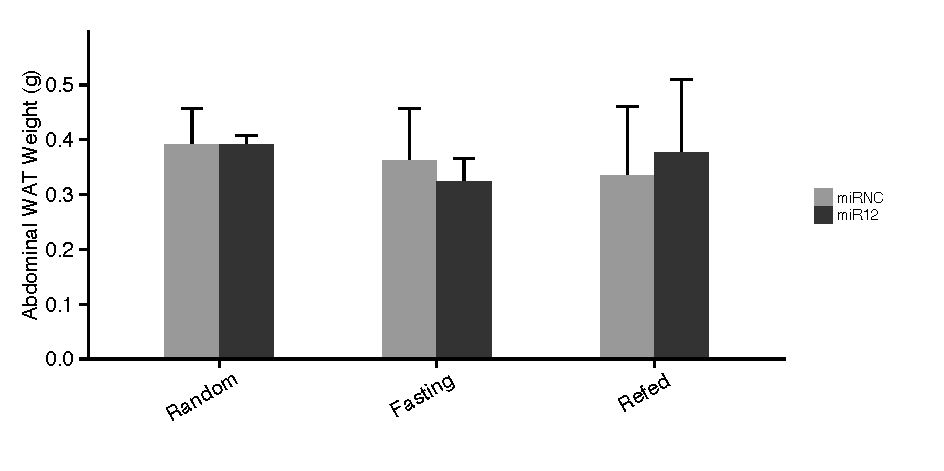
\includegraphics[width=1\textwidth]{figs/fig2-25 abd wat weight.pdf}
\caption[Abdominal fat after PPP2R5C KD]{\footnotesize Abdominal white adipose tissue (Abd.WAT) has no change after PPP2R5C knockdown. Mice were the same as Figure~\ref{fig:fig2.21}. After mice were treated with different nutritional statuses (Random, Fasting and Refed), Abd.WAT tissue was collected from each mouse and weighted before stored in -80\celsius{}. n=5 or 6.}
\label{fig:fig2.25}
\end{figure}

\subsection{PPP2R5C KD promotes glucose uptake \textit{in vivo} with better insulin sensitivity}

Since the liver is important for maintaining euglycemia, especially in the postprandial phase \cite{moore_regulation_2012}, I measured the blood glucose level for \textit{ad libitum} feeding ("Random"), 16 hour fasting ("Fasting"), and 16 hour fasting followed by 6 hour refeeding ("Refed") in control and knockdown mice (Figure~\ref{fig:fig2.26}). Surprisingly, there are no significant decreases in all three conditions, even given that PPP2R5C KD in cultivated hepatocytes increased glucose uptake (Figure~\ref{fig:fig2.15}). 

Although there is no change in blood glucose level after \gls{ppp2r5c} knockdown, the serum insulin concentration drops almost 2-fold after PPP2R5C knockdown (Figure~\ref{fig:fig2.28}) when mice are fed \textit{ad libitum}. In Fasting and Refed group, serum insulin levels are also decreased comparing with control mice. The decreased circulating insulin levels indicated the increased insulin sensitivity. Indeed, the insulin sensitivity index \cite{wallace_use_2004} in random and refed group are also increased in PPP2R5C knockdown mice (Figure~\ref{fig:fig2.29}). 

\begin{figure}[htbp]
\centering
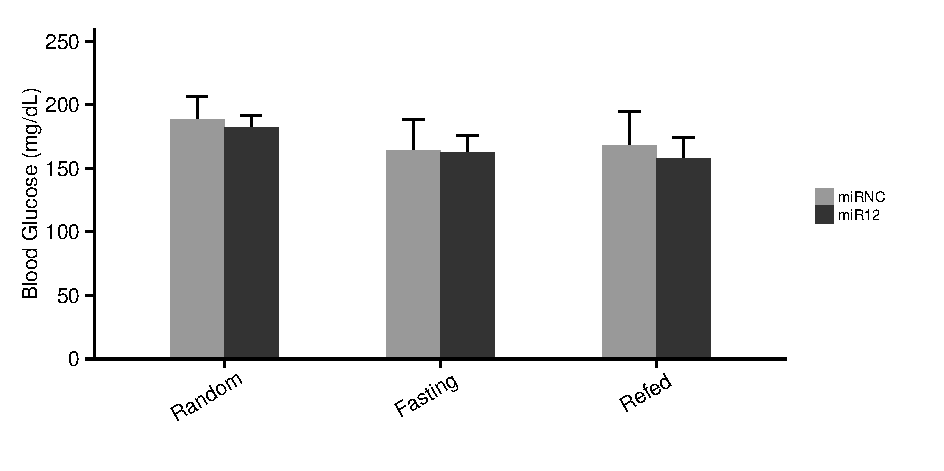
\includegraphics[width=1\textwidth]{figs/fig2-26 blood glucose.pdf}
\caption[Blood glucose after PPP2R5C KD]{\footnotesize Blood glucose level has no change after PPP2R5C knockdown. Mice were the same as Figure~\ref{fig:fig2.21}. Blood glucose level was immediately measured after sacrifice. n=5 or 6.}
\label{fig:fig2.26}
\end{figure}

\begin{figure}[htbp]
\centering
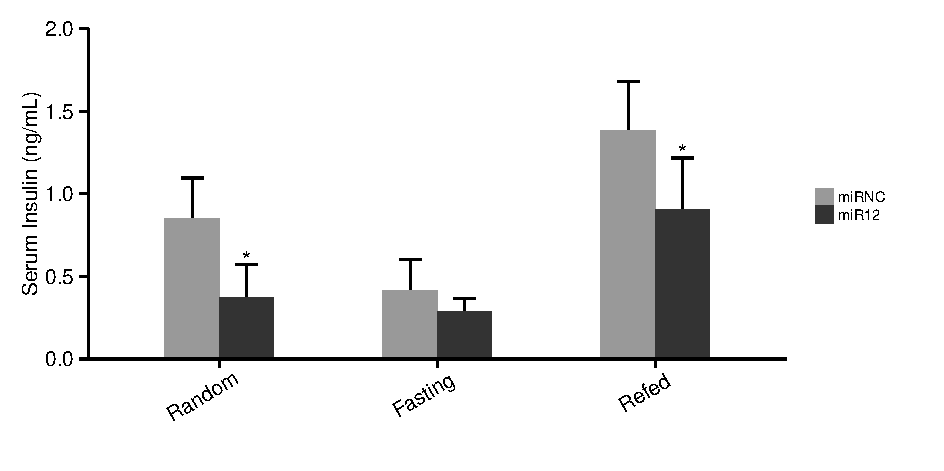
\includegraphics[width=1\textwidth]{figs/fig2-28 serum insulin.pdf}
\caption[Serum insulin drops after PPP2R5C KD]{\footnotesize Serum insulin drops after PPP2R5C knockdown in \textit{ad libitum} fed (Random) or 6-hour Refeeding after 16-hour fasting. Serum insulin was measured using ELISA kit for mouse insulin, and standard curve for ELISA was fitted from serial diluted insulin standards (0.1-6.9 ng/mL) with 5-parameter logistic model in R. * for p-value<0.05 by t-test in R for comparing miR12 to miRNC for each nutrition group. n=5 or 6.}
\label{fig:fig2.28}
\end{figure}


\begin{figure}[htbp]
\centering
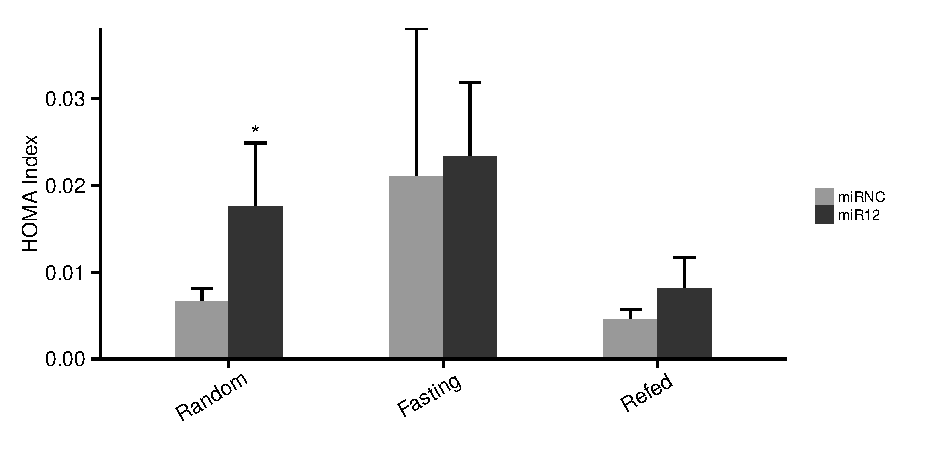
\includegraphics[width=1\textwidth]{figs/fig2-29 homa index.pdf}
\caption[ISI index increases after PPP2R5C KD]{\footnotesize Insulin sensitivity index (ISI) increases after PPP2R5C knockdown in \textit{ad libitum} fed (Random) or 6-hour re-feeding after 16-hour fasting. ISI index was calculated from the inverse of the product between blood glucose concentration and insulin concentration. * for p-value<0.05 by t-test in R for comparing miR12 to miRNC for each nutrition group. n=5 or 6}
\label{fig:fig2.29}
\end{figure}

Besides the increased insulin sensitivity, glucose uptake capacity is also increased in 6 hour fasted mice after \gls{ppp2r5c} knockdown, which is shown by the improved glucose tolerance in glucose tolerance test (GTT) (Figure~\ref{fig:fig2.43}). This piece of data is nicely correlated with the increased glucose uptake and glycolysis in cellular models (Hepa 1-6 cells and mouse primary hepatocytes, \cref{fig:fig2.11,fig:fig2.14,fig:fig2.15}). AUC analysis for \gls{gtt} data also demonstrates the decreased AUC in PPP2R5C knockdown (Figure~\ref{fig:fig2.44}). Although the absolute serum insulin levels from the same mouse in GTT experiment could not be calculated due to their level are below the limit of detection, raw O.D. 450 is used to estimate relative serum insulin level (Figure~\ref{fig:fig2.45}). And the relative serum insulin levels in PPP2R5C knockdown mice are even lower than control mice, given that they still have quicker glucose clearance rate (Figure~\ref{fig:fig2.43}). In sum, these data indicate PPP2R5C liver-specific knockdown mice have both increased insulin sensitivity and glucose uptake. 

\begin{figure}[htbp]
\centering
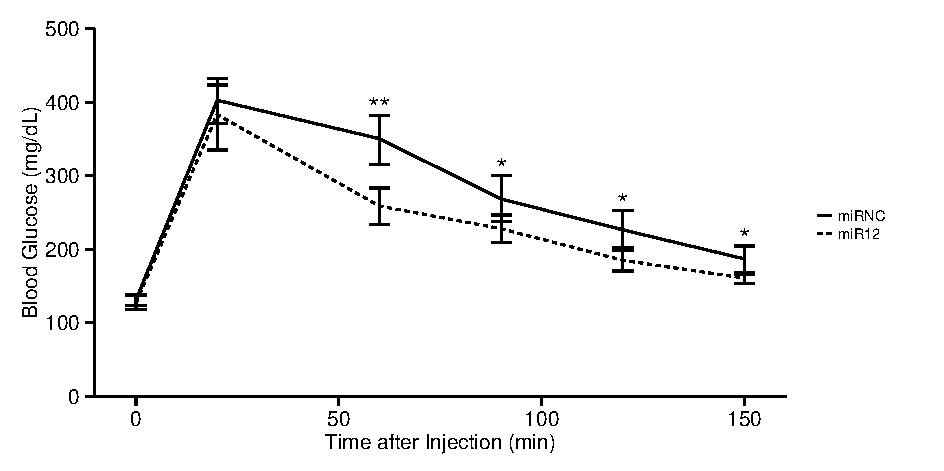
\includegraphics[width=1\textwidth]{figs/fig2-43 gtt.pdf}
\caption[GTT shows better glucose tolerance in PPP2R5C KD]{\footnotesize Glucose tolerance test (GTT) shows better glucose tolerance in PPP2R5C KD. GTT was performed 4 weeks after virus injection at dosage of 2g glucose/kg body weight. Glucose was solubilized in PBS and injected intraperitoneally. Blood glucose before injection was recorded as it for time 0 min, and also measured at time 20, 60, 90, 120 and 150 min. * and ** for p-value<0.05 and 0.01 by Wilcoxon signed-rank test in R for comparing miR12 to miRNC. n=12. Repeated Measures \gls{ANOVA} in R showed a significant difference in blood glucose changing profile with p-value of 0.0098.}
\label{fig:fig2.43}
\end{figure}

\begin{SCfigure}
\centering
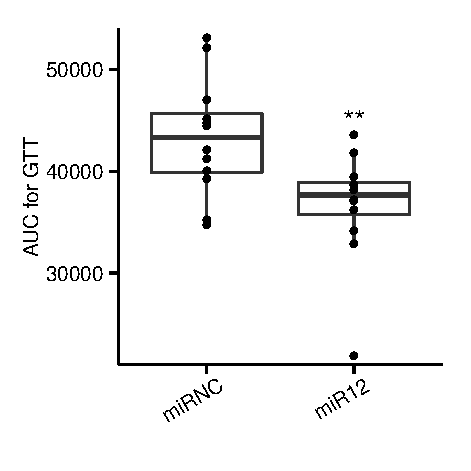
\includegraphics[width=0.5\textwidth]{figs/fig2-44 AUC for gtt.pdf}
\caption[AUC analysis for GTT results]{\footnotesize Area Under Curve (AUC) analysis for GTT blood glucose profile in Figure~\ref{fig:fig2.43}. ** for p-value<0.01 by t-test in R for comparing miR12 to miRNC. n=12.}
\label{fig:fig2.44}
\end{SCfigure}


\begin{figure}[htbp]
\centering
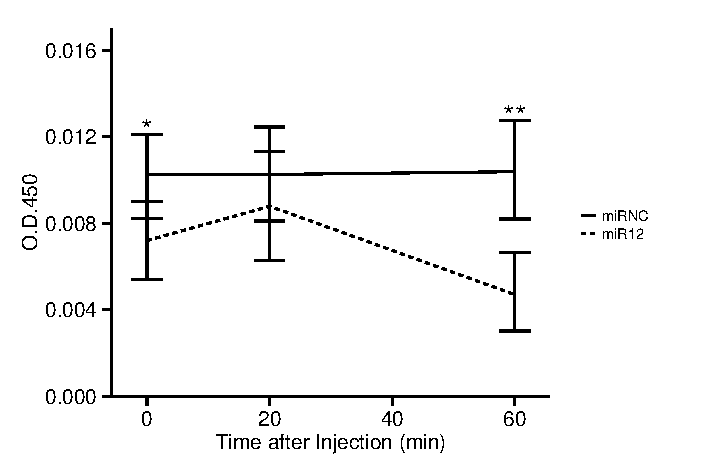
\includegraphics[width=1\textwidth]{figs/fig2-45 serum ins for gtt.pdf}
\caption[Serum insulin level in GTT]{\footnotesize Serum insulin relative level decreases in PPP2R5C. Due to O.D. 450 for some mice were even below the blank sample in the standard curve, absolute serum insulin level could not be calculated properly. Instead, raw O.D. 450 was employed to show the relative serum insulin level in GTT samples. * and ** for p-value<0.05 and 0.01 by two-sample t-test in R for comparing miR12 to miRNC. Repeated Measures \gls{ANOVA} in R showed a significant difference in serum insulin raw O.D. 450 profile with p-value of 0.0061. n=12.}
\label{fig:fig2.45}
\end{figure}


\subsection{PPP2R5C KD promotes anabolic changes in liver}

The increased glucose uptake in the liver after PPP2R5C KD indicates a more anabolic metabolism in hepatocytes in knockdown mice. In agreement with this, the liver has significant weight gain upon \gls{ppp2r5c} knockdown in all groups (Figure~\ref{fig:fig2.27}), instead of no systematic anabolic change in whole body weight or size of tissues beside the liver  (\cref{fig:fig2.22,fig:fig2.25}). The increase in Fasting and Refed group are even stronger than that in the Random group. In the postprandial phase, glucose is absorbed by hepatocytes to synthesize glycogen and lipids \cite{bechmann_interaction_2012,dashty_quick_2013}. The increase could be partially explained by the increase in liver glycogen (Figure~\ref{fig:fig2.30}) and triglyceride (Figure~\ref{fig:fig2.31}), even all these data are normalized to the liver weight. Without normalization, the increase in total liver triglyceride and glycogen would be even more.  Most strikingly, although glycogen levels drop in control livers upon fasting, as they enter a catabolic state to provide the rest of the organism with glucose, PPP2R5C knockdown livers displayed almost no drop in glycogen upon fasting (Figure~\ref{fig:fig2.30}).    

\begin{figure}[htbp]
\centering
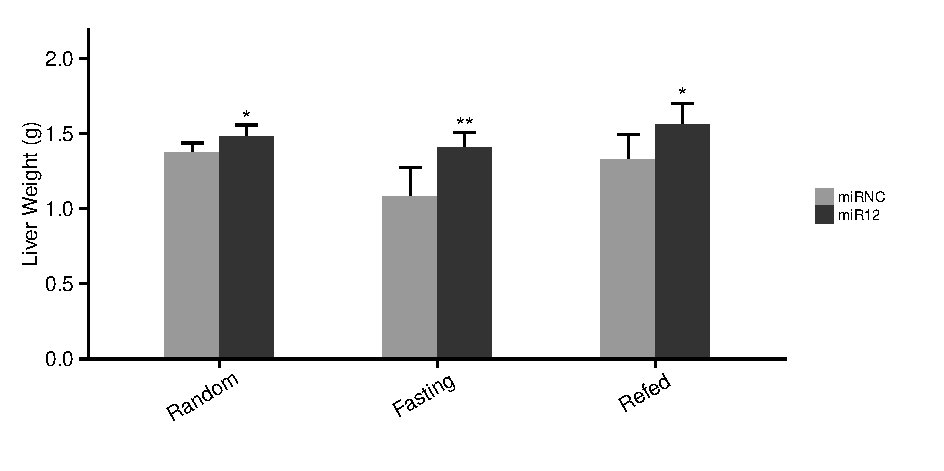
\includegraphics[width=1\textwidth]{figs/fig2-27 liver weight.pdf}
\caption[Liver weight increases after PPP2R5C KD]{\footnotesize Liver weight increases after PPP2R5C knockdown in all nutritional status. Mice were the same as in Figure~\ref{fig:fig2.21}. Dissected liver was weighted before aliquoting for cryosection, paraformaldehyde fixation and -80\celsius{} storage. n=5 or 6.}
\label{fig:fig2.27}
\end{figure}

\begin{figure}[htbp]
\centering
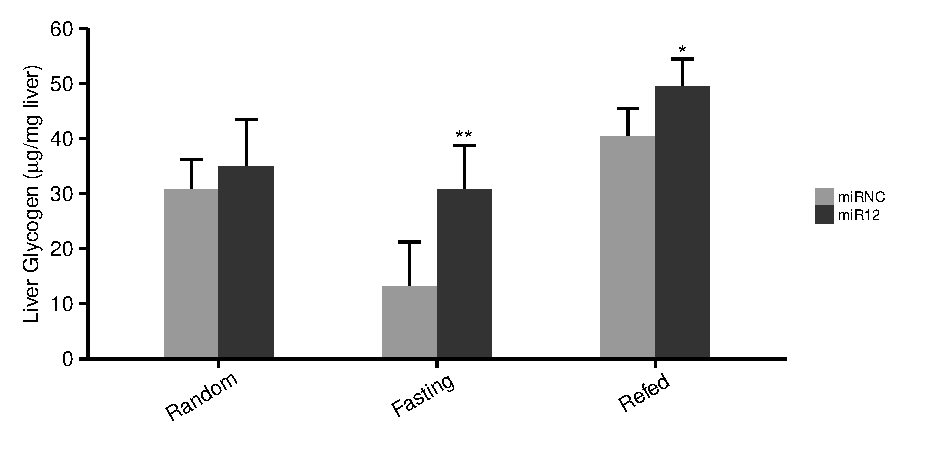
\includegraphics[width=1\textwidth]{figs/fig2-30 liver glycogen.pdf}
\caption[Liver glycogen increases after PPP2R5C KD]{\footnotesize Liver glycogen increases after PPP2R5C knockdown in fasting and refed. Mice were the same as in Figure~\ref{fig:fig2.21}. Frozen liver sample was pulverized in the tissue homogenizer with pre-cooling in liquid nitrogen. Glycogen was extracted from \textasciitilde150 mg liver powder and measured for glucose level after overnight amyloglucosidase digestion. * and ** for p-value<0.05 and 0.01 by t-test in R for comparing miR12 to miRNC for each nutrition group. n=5 or 6. }
\label{fig:fig2.30}
\end{figure}

Glucose is also used by hepatocytes for lipid biosynthesis. Combining data from \gls{gtt} experiment (Figure~\ref{fig:fig2.43}) and cell-autonomous increased glucose uptake lipogenesis in \textit{in vitro} cultivated hepatocytes (\cref{fig:fig2.15,fig:fig2.16}), implies the increased glucose uptake in the liver would also possibly shunted into lipid synthesis pathway. In agreement with this, mice with \gls{ppp2r5c} KD have significantly elevated triglyceride levels in their livers in the random feeding state. Due to two outliers of liver NEFA (Figure~\ref{fig:fig2.33}) in control mice in the random group, liver triglyceride levels in these two control mice are also higher, probably by passively increasing the re-esterification of NEFA into triglycerides in these two control mice. By \gls{ancova} (Analysis of Covariance) analysis with the liver NEFA as covariate, liver triglyceride in knockdown mice in the random group is found to be significantly higher (p-value=0.04). 

Although this lipid storage effect is visible after 7 week PPP2R5C knockdown (Figure~\ref{fig:fig2.31}), it is even more pronounced after 2 week knockdown (Figure~\ref{fig:fig2.57}), possibly due to the reduced knockdown efficiency upon counter-regulation over time, or compensatory regulatory mechanism developed over time. However, Oil Red O staining on the liver sample does not show visible change in lipid droplet (data not shown), which indicates the increased triglyceride storage is mainly microvesicular lipid droplets which are not easily visible under microscope after Oil Red O staining. 

\begin{figure}[htbp]
\centering
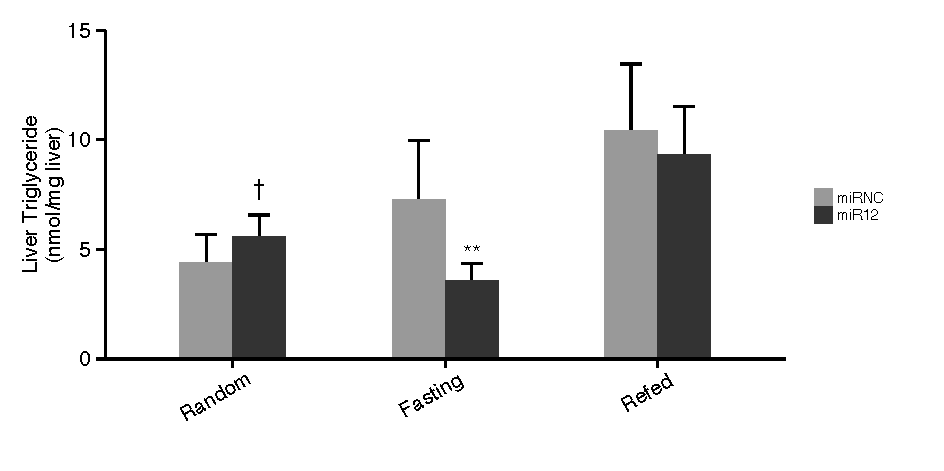
\includegraphics[width=1\textwidth]{figs/fig2-31 liver tag.pdf}
\caption[Liver triglyceride changes after PPP2R5C KD]{\footnotesize Liver triglyceride increases after PPP2R5C knockdown in random but decreases in fasting. Mice were the same as in Figure~\ref{fig:fig2.30}. Lipid fraction was extracted from liver by methanol-chloroform and triglyceride was measured as free glycerol released from lipase digestion. $\dagger$ for p-value<0.05 for \gls{ancova} analysis for comparing liver triglyceride between miRNC and miR12 in random fed, in which liver non-esterified fatty acids (\gls{nefa}) (Figure~\ref{fig:fig2.33}) as co-variate. ** for p-value<0.01 by t-test in R. n=5 or 6.}
\label{fig:fig2.31}
\end{figure}

\begin{figure}[htbp]
\centering
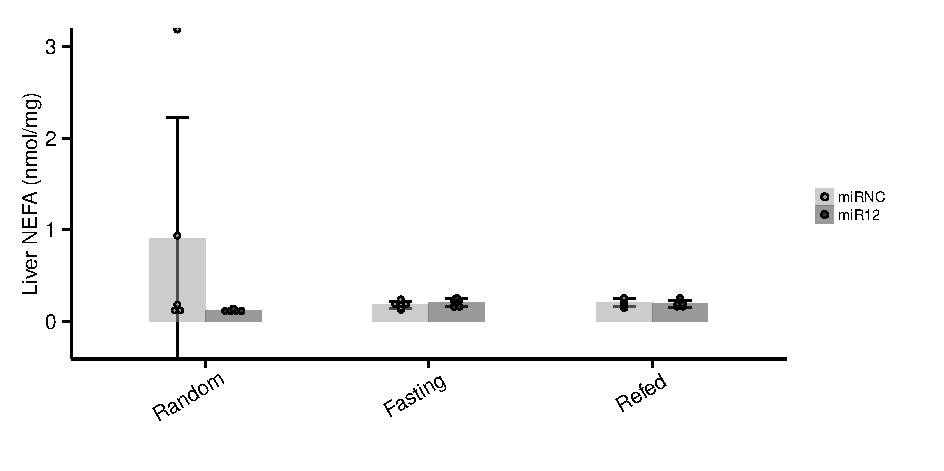
\includegraphics[width=1\textwidth]{figs/fig2-33 liver NEFA.pdf}
\caption[Liver NEFA has no change after PPP2R5C KD]{\footnotesize Liver NEFA level has no significant change after PPP2R5C knockdown in all feeding regimes. Mice were the same as in Figure~\ref{fig:fig2.30}. Lipid fraction was extracted from liver by methanol-chloroform and NEFA was measured. n=5 or 6.}
\label{fig:fig2.33}
\end{figure}

\begin{SCfigure}
\centering
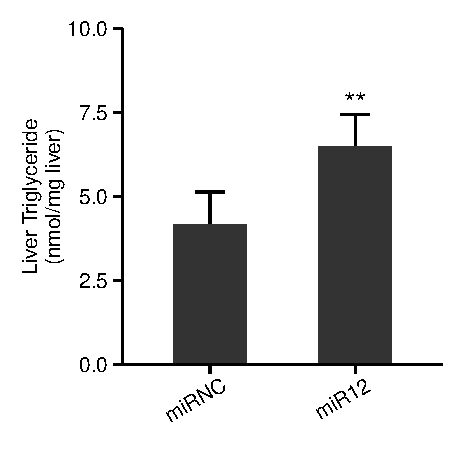
\includegraphics[width=0.5\textwidth]{figs/fig2-57 liver pilot tag.pdf}
\caption[Liver triglyceride increases in the pilot experiment]{\footnotesize Liver triglyceride increases after PPP2R5C knockdown in random fed. 8-10 week CL57BL/6 male mice were injected with adeno-associated virus packaged miRNA against mouse PPP2R5C (miR12) or scramble miRNA (miRNC) at 0.5 or 1$\times$10\textsuperscript{11} viral particles/mouse via tail injection in 100 $\mu$L PBS. And Injected mice was sacrificed after 2-week knockdown. For liver triglyceride analysis, data from low and high dose virus injection were combined. ** for p-value<0.01 by t-test in R for comparing miR12 to miRNC. n=5.}
\label{fig:fig2.57}
\end{SCfigure}


One possible explanation for the increased liver triglyceride levels could be the reduced liver fatty acid \textbeta{}-oxidation. However, the serum ketone body concentration of total ketone body species and hydroxybutyrate are maintained at the same level after \gls{ppp2r5c} KD (\cref{fig:fig2.37,fig:fig2.38}) at various feeding conditions. Total ketone body concentration are increased in the fasting group and decreased after refeeding for both control and PPP2R5C mice, which is expected since starvation in mice would increase \textbeta{}-oxidation activity in the liver and the following ketone body concentration in the circulation. Additionally, the hydroxybutyrate concentration normalized to total ketone body also did not show any relative change upon PPP2R5C KD (Figure~\ref{fig:fig2.39}). Circulating ketone body levels are not changed upon PPP2R5C KD is indicating that accumulation of hepatic triglyceride levels are not likely due to the impaired utilization in \textbeta{}-oxidation but presumably due to the increased \textit{de novo} lipogenesis, which have been demonstrated in \textit{in vitro} cell culture models (\cref{fig:fig2.16,fig:fig2.18}). 

\begin{figure}[htbp]
\centering
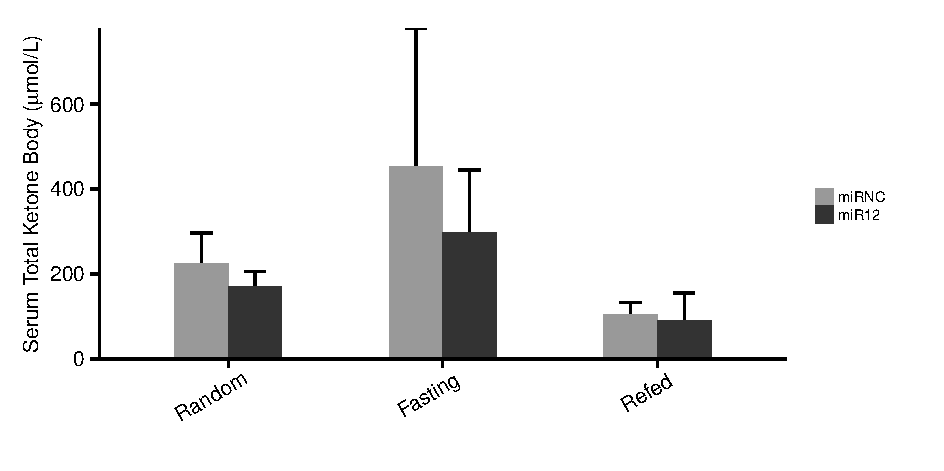
\includegraphics[width=1\textwidth]{figs/fig2-37 serum TKB.pdf}
\caption[Serum total ketone body upon PPP2R5C KD]{\footnotesize Serum total ketone body (TKB) does not change upon PPP2R5C knockdown in all feeding regimes. Mice were the same as in Figure~\ref{fig:fig2.30}. n=5 or 6.}
\label{fig:fig2.37}
\end{figure}

\begin{figure}[htbp]
\centering
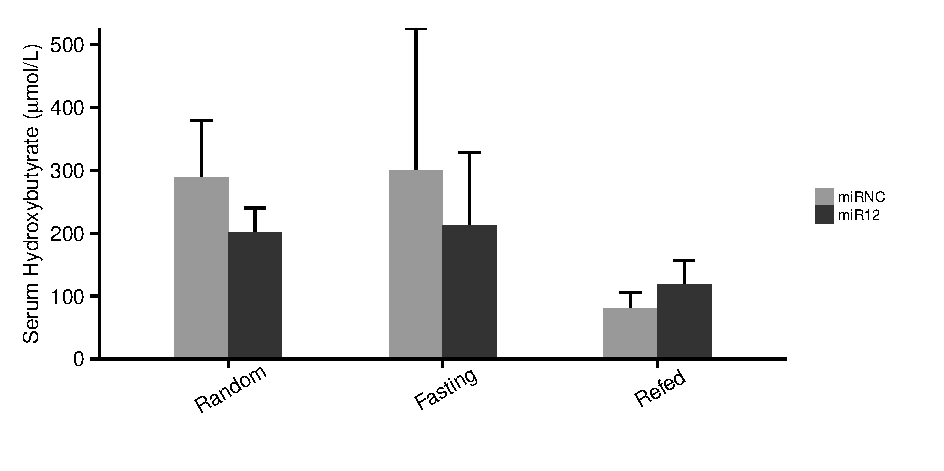
\includegraphics[width=1\textwidth]{figs/fig2-38 serum HB.pdf}
\caption[Serum hydroxybutyrate upon PPP2R5C KD]{\footnotesize Serum hydroxybutyrate (HB) concentration does not change upon PPP2R5C knockdown in all feeding regimes. Mice were the same as in Figure~\ref{fig:fig2.30}. n=5 or 6.}
\label{fig:fig2.38}
\end{figure}

\begin{figure}[htbp]
\centering
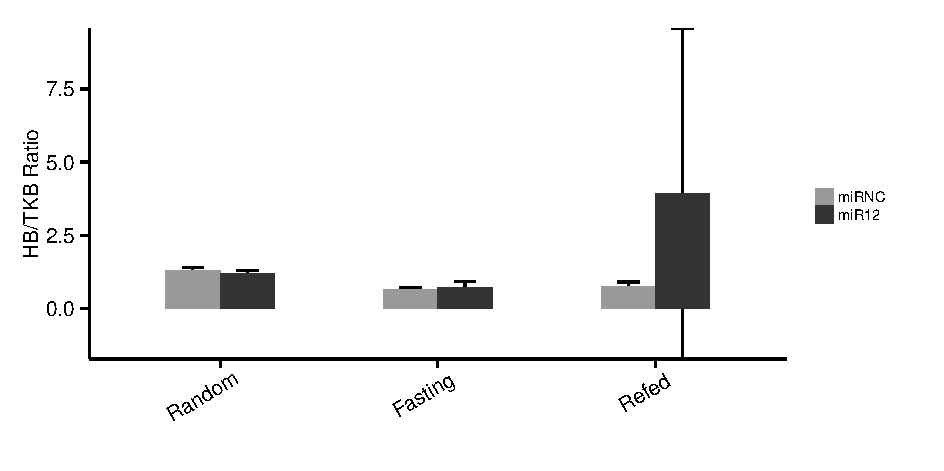
\includegraphics[width=1\textwidth]{figs/fig2-39 serum KB ratio.pdf}
\caption[Serum HB to TKB ratio upon PPP2R5C KD]{\footnotesize Serum HB to TKB ratio does not change upon PPP2R5C knockdown in all feeding regimes. Mice were the same as in Figure~\ref{fig:fig2.30}. n=5 or 6.}
\label{fig:fig2.39}
\end{figure}

Surprisingly, liver triglyceride levels drop significantly in PPP2R5C knockdown upon fasting (Figure~\ref{fig:fig2.31}). I have tested if this could be due to increased lipid secretion from the liver. Indeed, the serum triglyceride in fasting and refed group after PPP2R5C KD are increased significantly (Figure~\ref{fig:fig2.32}). This leads to a drop not only in triglyceride but also cholesterol in PPP2R5C knockdown livers upon fasting and refed (Figure~\ref{fig:fig2.35}). This raises the possibility of co-transportation of triglyceride and cholesterol out from the liver in the form of VLDL. Upon refeeding, PPP2R5C knockdown livers re-accumulated triglycerides very rapidly, reaching control levels within 6 hours of refeeding (Figure~\ref{fig:fig2.31}), consistent with elevated lipid biosynthesis rates in PPP2R5C knockdown livers. Taken together, PPP2R5C knockdown livers have more glucose uptake than control livers, thereby produce more triglycerides, and secrete elevated lipid amounts into circulation. The steady state levels of triglyceride in PPP2R5C knockdown livers likely reflect this balance between increased biosynthesis and increased secretion, leading to a drop in the liver triglyceride upon fasting when less dietary glucose is available for lipid biosynthesis. If the serum triglyceride and liver triglyceride are considered together, the overall triglyceride at least in random and refed condition are increased in knockdown mice.

\begin{figure}[htbp]
\centering
\includegraphics[width=1\textwidth]{figs/fig2-32 serum tag.pdf}
\caption[Serum triglyceride changes after PPP2R5C KD]{\footnotesize Serum triglyceride increases after PPP2R5C knockdown in fasting and refed. Mice were the same as in Figure~\ref{fig:fig2.30}. 2 $\mu$L serum from these mice was measured as free glycerol released from lipase digestion. ** and *** for p-value<0.01 and 0.001 by t-test in R. n=5 or 6.}
\label{fig:fig2.32}
\end{figure}

Lipoactive hormones such as epinephrine, norepinephrine, glucagon, thyrotropin, and adrenocorticotropin release free fatty acids (Serum \gls{nefa}) into serum from lipolysis in adipose tissues. And the liver can re-absorb almost 75\% of the serum NEFA to re-esterify them into triglyceride and release into serum as VLDL particle. Upon \gls{ppp2r5c} knockdown, the steady state level of serum NEFA in random and fasting feeding regime are not changed (Figure~\ref{fig:fig2.34}), which further indicates the increased lipid storage is rather sourced from \textit{de novo} lipogenesis in the liver. In refeeding, mice with PPP2R5C knockdown even have significant increased serum NEFA. During refeeding, serum NEFA could also be originated from the food intake. And it is possible the liver lipid synthesis capacity has already reached its plateau and the NEFA is accumulated in the serum to have a higher concentration in PPP2R5C knockdown mice than the control. This postulation also fits with the fact that the liver triglyceride in refed condition stays at very high level but there is still more triglyceride released into serum, which suggests higher triglyceride synthesis and secretion in the liver during refed.

\begin{figure}[htbp]
\centering
\includegraphics[width=1\textwidth]{figs/fig2-34 serum NEFA.pdf}
\caption[Serum NEFA changes in refed]{\footnotesize Serum NEFA is decreased in refed. Mice were the same as in Figure~\ref{fig:fig2.30}. Lipid fraction was extracted from liver by methanol-chloroform and triglyceride was measured as free glycerol released from lipase digestion. 2 $\mu$L serum from these mice was measured for NEFA. * for p-value<0.05 by t-test in R. n=5 or 6.}
\label{fig:fig2.34}
\end{figure}


\section{PPP2R5C negatively regulates VLDL secretion in the liver}

Given the fact that serum triglyceride was increased during fasting and refed, I performed a more detailed analysis of serum lipid composition by \gls{fplc} (Fast Performance Liquid Chromatography) fractionation of serum, in order to find which lipoprotein particle was responsible for increased serum triglyceride. \gls{vldl}, \gls{idl}, \gls{ldl} and \gls{hdl} could be nicely separated on a high resolution size-exclusion chromatography column. In Random group, mice after \gls{ppp2r5c} KD has no difference in serum lipoprotein particle profile (Total protein content (A280) in lipoprotein fractions is shown in Figure~\ref{fig:fig2.42}). However, there is a significant increase in \gls{vldl} fraction (approximately 5-fold increase) in Fasting and Refed group after PPP2R5C knockdown. In Fasting group, even there is a slight increase in HDL intensity, the relative VLDL intensity normalized to HDL is still increasing dramatically in knockdown mice. 

\begin{figure}[htbp]
\centering
\includegraphics[width=1\textwidth]{figs/fig2-42 fplc_profile.pdf}
\caption[Serum FPLC profile]{\footnotesize Increased VLDL fraction after PPP2R5C KD. Serum lipoprotein particles were analyzed by FPLC. 200 $\mu$L pooled serum from 5 or 6 mice in the same virus and feeding group was subjected to FPLC separation on high-resolution size-exclusion chromatography. FPLC profile was recorded as UV 280nm, which was the indicator for protein concentration. Separated serum was collected in fractions of 0.5 mL. Mice were the same as in Figure~\ref{fig:fig2.30}.}
\label{fig:fig2.42}
\end{figure}

Concordantly, triglyceride distribution profile in serum is also agreed with increased VLDL intensity (Figure~\ref{fig:fig2.40}). Although triglyceride concentrations in knockdown mice from Refed group have higher background level, the background subtracted intensity of VLDL triglyceride peak is distinctly higher than that for control mice in the same feeding group. Quantification of VLDL peak apex and peak area both in FPLC and triglyceride profile is shown in Figure~\ref{fig:fig2.58}. VLDL particles are lipoprotein particles synthesized in the liver and secreted into the blood stream for transporting endogenous triglyceride, cholesterol, phospholipids and cholesterol esters \cite{gibbons_synthesis_2004}. Comparing with other lipoprotein particles, VLDL has the highest percentage of triglyceride, and could explain the significant increase in serum triglyceride in the form of VLDL. The increased VLDL secretion is also observed in human upon increased hepatic \textit{de novo} lipogenesis \cite{schwarz_hepatic_2003}. 


\begin{figure}[htbp]
\centering
\includegraphics[width=1\textwidth]{figs/fig2-40 fplc_tag.pdf}
\caption[Triglyceride concentration in lipoprotein particles]{\footnotesize Triglyceride concentration profile correlated with its FPLC profile. 160 $\mu$L from each fraction was used to measure triglyceride concentration as free glycerol released from lipase digestion.}
\label{fig:fig2.40}
\end{figure}

\begin{figure}[htbp]
\centering
\includegraphics[width=1\textwidth]{figs/fig2-58 vldl_peak.pdf}
\caption[VLDL peak analysis]{\footnotesize Quantification of VLDL peak apex and area. Start and end point for each peak in Figure~\ref{fig:fig2.42} were manually selected by examining the emerging and vanishing time point for each peak comparing with the background. Peak Apex and Area were calculated in R by finding maximal intensity and trapezoid integration from start point to end point for VLDL peak.}
\label{fig:fig2.58}
\end{figure}

In agreement with the increased serum VLDL fraction, cholesterol level in this fraction has also increased (Figure~\ref{fig:fig2.41}), although contributes a small share in total serum cholesterol. The biggest cholesterol peak is from HDL, which is known to carry a high percentage of cholesterol. And this minor contribution from VLDL cholesterol also explain why there is no significant gain in the serum cholesterol level given the increased cholesterol secretion from the liver (Figure~\ref{fig:fig2.35}). Liver cholesterol is probably passively packaged into the VLDL particle together with the triglyceride and released into the serum, due to the increased lipogenesis in the liver upon PPP2R5C KD. However, the total serum cholesterol levels have not change (Figure~\ref{fig:fig2.36}) since the cholesterol from VLDL is only a minor fraction comparing to the cholesterol from IDL and HDL peaks (Figure~\ref{fig:fig2.41}), which are not changed dramatically upon PPP2R5C KD (Figure~\ref{fig:fig2.42}). This data further validates the hypothesis that increased glucose uptake in the liver is shunted into lipogenesis and eventually released into the serum in the form of \gls{vldl} after \gls{ppp2r5c} knockdown. 


\begin{figure}[htbp]
\centering
\includegraphics[width=1\textwidth]{figs/fig2-41 fplc_chol.pdf}
\caption[Cholesterol concentration in lipoprotein particles]{\footnotesize Cholesterol concentration profile in various lipoprotein particles. 40 $\mu$L from each fraction was used to measure cholesterol concentration.}
\label{fig:fig2.41}
\end{figure}


\begin{figure}[htbp]
\centering
\includegraphics[width=1\textwidth]{figs/fig2-35 liver chol.pdf}
\caption[Liver cholesterol drops upon PPP2R5C KD]{\footnotesize Liver cholesterol is dropped in fasting and refed after PPP2R5C KD. Mice were the same as in Figure~\ref{fig:fig2.30}. Lipid fraction was extracted from liver by methanol-chloroform and cholesterol was directly measured. * and ** for p-value<0.05 and 0.01 by t-test in R for comparing miR12 to miRNC for each nutrition group. n=5 or 6.}
\label{fig:fig2.35}
\end{figure}

\begin{figure}[htbp]
\centering
\includegraphics[width=1\textwidth]{figs/fig2-36 serum chol.pdf}
\caption[Serum cholesterol level remains no change]{\footnotesize Serum cholesterol has no change after PPP2R5C KD in all feeding regimes. Mice were the same as in Figure~\ref{fig:fig2.30}. 2 $\mu$L serum was used to measure cholesterol directly. n=5 or 6.}
\label{fig:fig2.36}
\end{figure}

In summary, due to the increased lipogenesis derived from the increased glucose uptake in the liver after PPP2R5C KD, VLDL secretion from the liver is also increased and contributing to the anabolic storage of glucose in the liver. The increased glucose clearance capacity of the liver after PPP2R5C KD enable the efficient euglycemic control with less insulin secretion from the pancreas in the postprandial phase or massive oral or enteral glucose load (like GTT). The increased glucose absorbed by the liver is  directed either to glycogen synthesis or lipid storage and secretion. It is known that the hepatic glycogen deposition is partially driven by the increased liver glucose uptake, metabolite or hormonal signaling from port vein, and partly by gluconeogenesis pathway \cite{radziuk_hepatic_2001}. In PPP2R5C knockdown mice, the increased glucose uptake will probably also explain the increased liver glycogen phenotype. Another possible anabolic change after increased glucose uptake is storing glucose as triglyceride through \textit{de novo} lipogenesis. The increased glucose flux to the liver after PPP2R5C KD could potentially activate lipogenic gene expression via multiple pathways. Glucose is considered as signaling metabolite for activating glycolytic and lipogenic pathways \cite{foufelle_new_2002}. In following sections, I will have more data to show the direct and indirect link from PPP2R5C to glucose metabolism.


\section{PPP2R5C's substrates in metabolism control}

\subsection{PPP2R5C's substrates include multiple metabolic regulators}

\gls{ppp2r5c} is a regulatory subunit of \gls{PP2A}, thought to provide substrate specificity to the phosphatase holoenzyme. However, given the phenotype I have observed from \textit{in vitro} and \textit{in vivo} knockdown of PPP2R5C, it is not possible to make a direct link from PP2A to the negative regulation of glycolysis and lipogenesis. There must be some intermediate molecular links from PP2A to the regulation of glycolysis and lipogenesis, such as glycolytic and lipogenic gene activation by some transcription factors and kinases. A reasonable educational guess is that PPP2R5C regulates glycolytic and lipogenic gene activation through de-phosphorylating metabolic regulators. 

Therefore, I performed a proteomic approach to identify target substrates that bind PPP2R5C. And potential substrates involved in metabolism control would provide a clue to elucidate the mechanism of PPP2R5C's negative regulation in glycolysis and lipogenesis. However, phosphatase substrate discovery is difficult. Beside occasionally successes in finding phosphatase interacting substrates, there are few reports regarding system-wide substrate identification for phosphatases, mostly protein tyrosine phosphatases \cite{boubekeur_new_2011,flint_development_1997,wu_identification_2006}. In the  case for protein tyrosine phosphatases, a substrate trapping mutant competes with its endogenous counterpart for substrates. Due to its structural simplicity (single subunit and verified catalytic dead mutant, usually a cysteine to serine mutation in catalytic active center), protein tyrosine phosphatase is much easier for pulling down its binding substrates. For Serine/Threonine kinases, MAP kinase phosphatase-1 is another success example of substrate trapping \cite{kinney_histone_2009}.

Protein-protein interactions between phosphatases and substrates are notoriously transient and difficult to detect via conventional methods, such as co-immunoprecipitation and pull-down strategies. I have tested these conventional methods and abandoned them for PPP2R5C substrate isolation due to the high background and no detectable new band on SDS-PAGE gel. Here in the thesis project, I employed the BioID method \cite{roux_promiscuous_2012}   to identify PPP2R5C interacting proteins, including its potential substrates. A fusion between PPP2R5C and the biotin ligase \gls{bira} mutant (BirA*) was expressed in Hepa 1-6 cells. The mutant biotin ligase (R118G) has been shown to be able to generate reactive biotin (biotin-5'-AMP) and ligate biotin onto proteins \textit{in vitro} \cite{choi-rhee_promiscuous_2004,cronan_targeted_2005}. With the co-expression of substrate trapping mutant of PP2A catalytic subunit C, fusion protein from PPP2R5C and BirA* led to \textit{in vivo} biotinylation of PPP2R5C interacting proteins, which can subsequently be isolated by collecting cellular lysates and streptavidin pulldown (Figure~\ref{fig:fig2.46}). 

By this way, these potential substrates with weak interactions with PPP2R5C would have a higher chance to be identified by the Western blot or mass spectrometry with very low background since it is possible to apply very stringent washing steps. BirA* was fused to either the N-terminus or the C-terminus of PPP2R5C (Myc-BirA-PPP2R5C and PPP2R5C-BirA-HA respectively), and Myc or HA-tagged BirA* alone was used as a negative control. In addition, the catalytic dead mutation (D85N), which was known to eliminate the phosphatase activity \cite{ogris_catalytically_1999} by disrupting the Mg\textsuperscript{2+} binding in the active center, was introduced into the catalytic subunit of \gls{PP2A} (PP2CA). This design was the first successful attempt to perform a substrate trapping assay for PP2A, and expected to employ \gls{PP2A}'s substrate-trapping mutation might extend the duration of interaction between \gls{PP2A} and its substrate proteins. Then there will be more \textit{in vivo} biotinylation on these substrates when the PP2A catalytic dead mutant is co-expressed. 

\begin{figure}[htbp]
\centering
\includegraphics[width=1\textwidth]{figs/fig2-46 bioID scheme.png}
\caption[PPP2R5C substrate trapping scheme]{\footnotesize PPP2R5C containing PP2A holoenzyme substrate trapping and \textit{in vivo} biotinylation of its substrates.}
\label{fig:fig2.46}
\end{figure}

In the BioID experiment, various known regulators of the liver metabolism were found to be interacting with \gls{ppp2r5c}, including \gls{AMPK} \textbeta{}1, \gls{HIF1a}, \gls{s6k}, \gls{stat3} (Figure~\ref{fig:fig2.47a}). Comparing to either Myc-\gls{bira}* or BirA*-HA controls, HIF1\textalpha{} has increased biotinylation, which is shown as stronger band after streptavidin pulldown and detection with total antibodies for individuals. When co-expressed with the substrate trapping mutant of \gls{PP2A} catalytic subunit, the interaction between PPP2R5C and its substrates is further increased. This proves the success of the substrate trapping mutant of PP2A, which could potentially increase the binding duration of substrates to PPP2R5C containing PP2A holoenzyme. For \gls{s6k} and \gls{stat3}, similar results are also observed and indicating their possibility of being PPP2R5C's substrates. With \gls{AMPK}'s various subunits tested in substrate trapping, including \textalpha{}, \textbeta{}1 and \textbeta{}2, only \textbeta{}1 subunit has been found to be a potential PP2A substrate. In contrast, no binding of PPP2R5C to SREBP-1, or a panel of negative control proteins are detected, including HSP90, YAP, TSC1 and RpL26 (Figure~\ref{fig:fig2.47b}).

\begin{figure}[!t]
\centering
	\begin{subfigure}[t]{0.48\textwidth}
	\subcaption{Western blot of PPP2R5C substrate}
	\includegraphics[width=1\textwidth]{figs/fig2-47 bioid target1.pdf}
    \label{fig:fig2.47a}
	\end{subfigure} %
~
	\begin{subfigure}[t]{0.48\textwidth}
	\subcaption{Negative controls of PPP2R5C substrate trapping}
	\includegraphics[width=1\textwidth]{figs/fig2-48 bioid target2.pdf}
    \label{fig:fig2.47b}
	\end{subfigure}
\caption[Metabolic regulators as PPP2R5C's substrates]{\footnotesize PPP2R5C's substrates involved in metabolic control. (a) PPP2R5C interacting proteins were validated by western blot. SREBP-1, Tubulin or Actin were used as non-interacting controls. (b) AMPK \textbeta{}1 subunit and several other negative controls were used to validate the specificity of PPP2R5C's substrate trapping in an independent repeat experiment.}
\label{fig:fig2.47}
\end{figure}


\subsection{AMPK is PPP2R5C's substrate involved in glucose uptake}

The \gls{AMPK} is a master regulator in energy homeostasis. It is a trimeric heterogenous complex composed of \textalpha{} for catalytic activity, \textbeta{} for regulatory function, and \textgamma{} for sensing AMP/\gls{ATP} ratio. Given the interaction between \gls{AMPK} \textbeta{}1 and \gls{ppp2r5c} (Figure~\ref{fig:fig2.47}), there might also be some functional link between \gls{PP2A} and \gls{AMPK}. Indeed, there were several reports showed the \gls{AMPK} phosphorylation is negatively regulated by \gls{PP2A} \cite{park_ampk_2013,wang_pp2a_2010,wu_activation_2007}. However, which regulatory subunit in \gls{PP2A} is responsible for \gls{AMPK} de-phosphorylation is still unknown. With PPP2R5C knockdown, the PPP2R5C containing sub-pool of \gls{PP2A} holoenzyme is reduced. \gls{AMPK} activity is markedly increased upon PPP2R5C knockdown with different methods, either the adenovirus mediated knockdown (Figure~\ref{fig:fig2.50a}) or an inducible shRNA stable cell line (Figure~\ref{fig:fig2.50b}). This data clearly shows that PPP2R5C is at least one of the regulatory subunit of \gls{PP2A} involved in \gls{AMPK} inhibition in liver originated cell lines. Accordingly, \gls{AMPK} activity change was further validated by the changes in its downstream effectors' activity such as ACC1 phosphorylation, TBC1D1 phosphorylation. For ACC1 phosphorylation, it has been well characterized as AMPK target and mediating AMPK's inhibition on lipogenesis \cite{ha_critical_1994,sullivan_inhibition_1994}. It is known that TBC1D1, the mouse homolog for human AS160, is an upstream regulator for Glut1 translocation and  phosphorylation at S700 of TBC1D1 promotes glucose uptake \cite{vichaiwong_contraction_2010,zhou_akt_2008}. This raises the possibility of AMPK activation after PPP2R5C knockdown is mediating the increased glucose uptake phenotype (\cref{fig:fig2.14,fig:fig2.15}).

\begin{figure}[htbp]
\centering
	\begin{subfigure}[t]{0.48\textwidth}
	\subcaption{AMPK activity increases upon PPP2R5C KD}
	\includegraphics[width=1\textwidth]{figs/fig2-50a ampk increase AV shR3.pdf}
    \label{fig:fig2.50a}
	\end{subfigure} %
~
	\begin{subfigure}[t]{0.48\textwidth}
	\subcaption{Activity increase of AMPK and its down-steam effectors}
	\includegraphics[width=1\textwidth]{figs/fig2-50b ampk increase.pdf}
    \label{fig:fig2.50b}
	\end{subfigure}
\caption[AMPK activity increases upon PPP2R5C knockdown]{\footnotesize AMPK activity is up-regulated upon PPP2R5C knockdown. (a) AMPK activity is increased after PPP2R5C knockdown by adenovirus packaged shR3 comparing to shRNC (PPP2R5C KD vs Control KD). (b) Inducible shR3 and shR6 (PPP2R5C KD1 and KD2) were used to examine the AMPK activity change in order to eliminate any virus-mediated effect in (a).}
\label{fig:fig2.50}
\end{figure}

\subsection{HIF1\texorpdfstring{\textalpha}{a}{} is PPP2R5C's substrate involved in glycolysis and lipogenesis}

The \gls{HIF1a} is also known for controling glycolysis and lipogenesis in the liver \cite{ochiai_disruption_2011,nath_hepatocyte-specific_2011,li_altered_2006,li_intermittent_2005, wang_ablation_2009}. The interaction between HIF1\textalpha{} and PPP2R5C, which is demonstrated by the substrate trapping in Figure~\ref{fig:fig2.47}, indicates that HIF1\textalpha{} could also be one of PPP2R5C's potential substrates involved in metabolism control. However, there is no phospho-specific antibody commercially available for HIF1\textalpha{}. Then I used Phos-tag\textsuperscript{\textregistered} gel to evaluate the functional relevance of PPP2R5C knockdown on HIF1\textalpha{}'s phosphorylation status (Figure~\ref{fig:fig2.51}). Phos-tag\textsuperscript{\textregistered} gel is made from an acrylamide analog containing chemical group for binding phosphorylated ions specifically \cite{tomida_detection_2008,kinoshita_improved_2011,marelli-berg_molecular_2012,hosokawa_quantitative_2010,kinoshita_separation_2009}. When protein is phosphorylated, its mobility in Phos-tag\textsuperscript{\textregistered} gel will be retarded. As a result, phosphorylated and non-phosphorylated proteins will be separated and protein phosphorylation with unknown site could be possibly examined without phospho-specific antibodies. The HIF1\textalpha{} has increased phosphorylated form upon PPP2R5C knockdown, and this phosphorylation is also validated by CIP treatment (Figure~\ref{fig:fig2.51}). These data suggest the PPP2R5C knockdown increases the phosphorylation of HIF1\textalpha{}.

\begin{figure}[htbp]
\centering
\includegraphics[width=0.9\textwidth]{figs/fig2-51 hif phospho.pdf}
\caption[HIF1\textalpha's phosphorylation analysis by Phos-tag\textsuperscript{\textregistered}]{\footnotesize HIF1\textalpha{}'s phosphorylation is increased after PPP2R5C KD. HIF1\textalpha{}'s phosphorylation status was evaluated in Phos-tag\textsuperscript{\textregistered} gel after inducible shR3 and shR6 expression (PPP2R5C KD1 and KD2).}
\label{fig:fig2.51}
\end{figure}

In agreement with the phosphorylation increase upon \gls{ppp2r5c} knockdown, \gls{HIF1a}'s transcriptional activity is also up-regulated after PPP2R5C knockdown (Figure~\ref{fig:fig2.53}) in mouse primary hepatocytes. Four canonical down-stream targets of HIF1\textalpha{} are all increased in mRNA level. Three of these four targets are involved in glycolysis, including LDH\textalpha{}, HK2, and PKM2, could help to explain the increased glycolysis after PPP2R5C knockdown. In addition, the activation of HIF1\textalpha{} in the mouse liver by hypoxia has been shown to activate SREBP-1 consequently and promote lipid accumulation in the liver \cite{li_intermittent_2005}. Interaction between HIF1\textalpha{} and PPP2R5C provides a possible indirect link from PPP2R5C KD to lipogenic gene activation, and elucidates the strong lipid storage phenotype in mouse primary hepatocytes after PPP2R5C KD (Figure~\ref{fig:fig2.16}). The next missing link in this hypothesis would be the SREBP-1 activation.

\begin{figure}[!tbp]
\centering
\includegraphics[width=1\textwidth]{figs/fig2-53 hif target 1st hepa.pdf}
\caption[HIF1\textalpha's transcriptional activity increases upon PPP2R5C KD]{\footnotesize HIF1\textalpha{}'s transcriptional activity is increased after PPP2R5C KD. Four HIF1\textalpha{}'s targets were examined for its total mRNA level in mouse primary hepatocytes after PPP2R5C KD.}
\label{fig:fig2.53}
\end{figure}

\subsection{Microarray analysis of PPP2R5C KD in mouse liver}\label{sec:sec254}

In parallel with the substrate trapping experiment,  I also performed the microarray analysis on PPP2R5C knockdown cells and tissue samples to shed more light on the mechanism behind the increased glycolysis and lipogenesis phenotype. Mouse primary hepatocytes, Hepa 1-6 cells and mouse livers with or without PPP2R5C were submitted for microarray analysis. For mouse liver samples, different feeding groups was also included. Differentially expressed gene list was generated based on 2-fold change cutoff for all feeding conditions and cell culture with PPP2R5C knockdown by the limma package in R. 

In order to find relevant transcription factors (TF) involved in the metabolic change and further link these TFs to PPP2R5C substrates, I performed an enrichment analysis for activated or inhibited TFs after PPP2R5C KD in mouse tissues or cell models. TF enrichment analysis was done with an online web server of TFactS \cite{essaghir_transcription_2010}. The TFactS analysis is analyzing the differentially expressed genes with 2-fold cutoff and finding the most possible TFs for these genes based on published known target genes of various TFs. The Transcription factor (TF) enrichment analysis from differentially expressed genes in mouse liver with PPP2R5C KD has shown the increased SREBP-1 activity after PPP2R5C KD both in cell and tissue samples (\cref{tab:tab2.1,tab:tab2.2,tab:tab2.3,tab:tab2.4}).

During refeeding, both SREBP-1 and HIF1\textalpha{} were enriched based on their potential target gene activation (Table~\ref{tab:tab2.1}). The activated TF lists upon PPP2R5C KD in fasting and random fed are shown in Supplementary \cref{tab:tab2.2,tab:tab2.3}. The activated TF list upon PPP2R5C KD in mouse primary hepatocyte and Hepa 1-6 is shown in Supplementary Table~\ref{tab:tab2.4}. All these lists have SREBP-1 (gene name SREBF1) in the activation TF list based on target gene expression. HIF1\textalpha{}, although only significant in FDR controlled p-value, is also enriched in activated TF list. The activation of HIF1\textalpha{} and SREBP-1 further supports HIF1\textalpha{} as potential PPP2R5C's substrate, and mediating the increased lipogenesis phenotype after PPP2R5C KD, possibly through the downstream activation of SREBP-1. 

\begin{table}[htbp]
\begin{center}
\begin{threeparttable}
\caption{Activated TFs in mouse liver upon PPP2R5C KD during refed.}
\label{tab:tab2.1}
\begin{footnotesize}
\begin{tabular}{lcc}
\toprule
\multicolumn{1}{c}{Transcription Factor}&\multicolumn{1}{c}{P-value}&\multicolumn{1}{c}{FDR control (B-H)\tnote{a}.}\tabularnewline
\midrule
\textbf{SREBF1}&$0.00038$&$0.001613$\tabularnewline
TP53&$0.00266$&$0.003226$\tabularnewline
ID3&$0.00921$&$0.004839$\tabularnewline
ID2&$0.00921$&$0.006452$\tabularnewline
NOTCH2&$0.01226$&$0.008065$\tabularnewline
ID1&$0.01226$&$0.009677$\tabularnewline
PPARA&$0.03340$&$0.011290$\tabularnewline
SMAD1&$0.04233$&$0.012900$\tabularnewline
NR2F1&$0.04825$&$0.014520$\tabularnewline
\textbf{HIF1A}&$0.06579$&$0.016130$\tabularnewline
STAT1&$0.07446$&$0.017740$\tabularnewline
E2F1&$0.07917$&$0.019350$\tabularnewline
FOXO1&$0.08369$&$0.020970$\tabularnewline
CEBPA&$0.09721$&$0.022580$\tabularnewline
SREBF2&$0.10000$&$0.024190$\tabularnewline
\bottomrule
\end{tabular}
\end{footnotesize}
\begin{tablenotes}  
\item[a] \scriptsize{Adjusted p-value (false discovery rate) by Benjamini-Hochberg method  \cite{benjamini_controlling_1995}}.
\end{tablenotes}
\end{threeparttable}
\end{center}
\end{table}


\subsection{SREBP-1 is involved in lipogenesis phenotype}

In Section~\ref{sec:sec254}, SREBP-1 is found to be activated upon PPP2R5C knockdown. Since SREBP-1 is the master regulator in lipogenesis, and its over-expression in the liver cause fatty liver \cite{horton_srebps:_2002}. Although SREBP-1 was not interacting with \gls{ppp2r5c} in substrate trapping experiment, SREBP-1 could still be involved in the lipogenesis phenotype after PPP2R5C KD in two possible ways. First, the decrease in the liver cholesterol in fasting and refed group indicates that SREBP-1 activity increase could be the direct result from liver cholesterol decrease due to the fact that the cholesterol and its derivatives are endogenous molecules have been demonstrated to regulated SREBP-1 expression \cite{amemiya-kudo_transcriptional_2002,wang_srebp-1_1994}. Decreased cholesterol concentration will relieve the cholesterol's suppression on SREBP-1 activity.  By this way, SREBP-1 is activated as a secondary effect from PPP2R5C KD. Secondly, SREBP-1 could also act as a downstream effector in \gls{HIF1a} mediated lipogenesis \cite{li_altered_2006}. The direct interaction between HIF1\textalpha{} and PPP2R5C, together with the evidence of HIF1\textalpha{} phosphorylation change and transcriptional activation, obviously indicates that SREBP-1 activation could also be an outcome of HIF1\textalpha{} activation. No matter the SREBP-1 activation is the primary or secondary consequences after PPP2R5C KD, it is inevitable that the SREBP-1 activation is a downstream consequence PPP2R5C KD, given that there is no interaction observed between PPP2R5C and SREBP-1. 

\begin{figure}[!t]
\centering
\includegraphics[width=1\textwidth]{figs/fig2-52 aav liver srebp insulin signal.pdf}
\caption[SREBP-1 protein increases upon PPP2R5C KD]{\footnotesize SREBP-1 protein level is increased after PPP2R5C KD. Insulin signaling activity was monitored by AKT and GSK3\textbeta{} phosphorylation.}
\label{fig:fig2.52}
\end{figure}

Indeed, the SREBP-1 activity is increased in the mouse liver upon \gls{ppp2r5c} knockdown when mice are subjected to fasting and refed (Figure~\ref{fig:fig2.52}). The SREBP-1 activation is represented by increased SREBP-1 precursor protein level in Fasting and Refed group. Since SREBP-1 can auto-activate itself, the increased precursor level clearly indicates an SREBP-1 activation. Also, the mature form of SREBP-1, which is the direct measurement of SREBP-1 activation, are also up-regulated both in Refed and Random fed group. In addition, the insulin signaling activity, represented by the AKT and GSK3\textbeta{} phosphorylation, is remained the same. This rules out the possibility that the increased SREBP-1 activity is originated from the insulin signaling, a positive regulator of SREBP-1 activity by increasing the SREBP-1 cleavage and maturation. 


\begin{figure}[!t]
\centering
\includegraphics[width=1\textwidth]{figs/fig2-54 srebp 1st hepa.pdf}
\caption[SREBP-1 activity increases upon PPP2R5C KD in primary hepatocytes]{\footnotesize SREBP-1 transcriptional activity is upregulated in PPP2R5C KD. Four SREBP-1's targets (DGAT2, GPAT1, ACLY, and SLC25A1 are all genes involved in lipogenesis) were examined for its total mRNA level in mouse primary hepatocytes after PPP2R5C KD.}
\label{fig:fig2.54}
\end{figure}

Additionally, qPCR analysis of several SREBP-1 target genes shows that the SREBP-1 transcriptional activity is also increased in mouse primary hepatocytes (Figure~\ref{fig:fig2.54}) and the mouse liver (Figure~\ref{fig:fig2.55}) after PPP2R5C knockdown. Four canonical SREBP-1 target genes involved in lipogenesis (\gls{DGAT2}, \gls{GPAT1}, \gls{ACLY}, and \gls{SLC25A1}) are all significantly up-regulated after PPP2R5C knockdown in mouse primary hepatocytes and mouse livers. Since SREBP-1 could auto-activate itself, increased SREBP-1 mRNA level is also observed in the mouse liver after PPP2R5C knockdown during fasting and refeeding (Figure~\ref{fig:fig2.55}). The transcriptional up-regulation of SREBP-1 itself is also fit with the observation in Figure~\ref{fig:fig2.52}. It is known that \gls{HIF1a} could still regulate the lipogenesis in the mouse liver \cite{wang_ablation_2009}, even the mice are not under hypoxia. Both HIF1\textalpha{} activity increase and cholesterol lowering after PPP2R5C knockdown would potentially increase the SREBP-1 activity, which promotes the \textit{de novo} lipogenesis. 

\begin{figure}[!tbp]
\centering
\includegraphics[width=1\textwidth]{figs/fig2-55 liver srebp.pdf}
\caption[SREBP-1 activity increased in mouse liver]{\footnotesize SREBP-1 transcriptional activity is upregulated in mouse liver after PPP2R5C KD. Total mRNA of SREBP-1 and its downstream targets in lipogenesis were investigated in mouse liver.}
\label{fig:fig2.55}
\end{figure}


In summary, PPP2R5C's substrate trapping and microarray analysis after PPP2R5C knockdown shed some light on how PPP2R5C could negatively regulate the glucose uptake, glycolysis and lipogenesis. AMPK and HIF1\textalpha{} can be PPP2R5C's direct downstream effectors in metabolism control. In the branch of glucose uptake and glycolysis, AMPK and HIF\textalpha{} could work in concert to promote the glucose absorption and glycolysis in hepatocytes. However, AMPK and HIF\textalpha{} seem to have an opposite function in regulating lipogenesis. On one hand, HIF1\textalpha{} activation will promote lipogenesis via SREBP-1. And on the other hand, AMPK activation after PPP2R5C KD could potentially inhibit \textit{de novo} lipogenesis via ACC1 phosphorylation \cite{sullivan_inhibition_1994} and inhibition on SREBP-1 cleavage at high fat diet fed mouse \cite{li_ampk_2011}. The exact function of this opposite control on lipogenesis is still unknown. However, a similar situation in signaling transduction has been reported frequently \cite{kuttykrishnan_quantitative_2010,goentoro_incoherent_2009}, and is so-called incoherent feed-forward loop. This special design would allow rhythmical activation of downstream signaling or avoiding over-shooting of the downstream activation signals \cite[Chapter 4]{alon_introduction_2006}. 

\section{Human PPP2R5C in Type 2 Diabetes}\label{sec:sec2.6}

\subsection{PPP2R5C's misregulation in human liver}

\begin{figure}[htbp]
\centering
\includegraphics[width=1\textwidth]{figs/fig2-60 human ppp2r5c vs t2d GIR.pdf}
\caption[Human PPP2R5C mRNA levels in human liver]{\footnotesize Human liver PPP2R5C mRNA levels correlate with T2D and GIR. PPP2R5C in healthy control (Control) and type 2 diabetic patients (T2D) was normalized to 18S rRNA level in liver, and shown as box-and-whisker plot (left panel). Human liver PPP2R5C is also negatively correlates with covariate GIR (glucose infusion rate). *** for p-value<0.001 by t-test in R for comparing Control to T2D. n=40 and 26 for Control and T2D respectively. Cohort study and qPCR experiments were performed by Prof. Matthias Bl\"uher, Nora Kl\"oting and Arne Dietrich in University of Leipzig, and analyzed by Yong-Sheng Cheng.}
\label{fig:fig2.60}
\end{figure}

In a cohort study of 76 liver samples from human, including 40 healthy donors and 26 type 2 diabetic patients (performed by my collaborator Prof. Matthias Bl\"uher in University of Leipzig), human PPP2R5C total mRNA levels were checked by quantitative PCR with 18S rRNA as the normalization control in Prof. Matthias Bl\"uher's lab. The human liver PPP2R5C mRNA is significantly increased in type 2 diabetes (Figure~\ref{fig:fig2.60}). The up-regulation of human PPP2R5C in type 2 diabetic patients is correlated with the findings that almost all variants of mouse PPP2R5C are increased in the liver of \textit{db/db} mice, which is a mouse genetic model for type 2 diabetes (Figure~\ref{fig:fig2.1}). This up-regulation in the human liver could be considered as  a negative feedback of PPP2R5C transcription in order to curtail the lipid synthesis capacity of the liver, or a potential reason for insulin resistance since PPP2R5C KD could improve insulin sensitivity. In type 2 diabetic patients, majority of them will accumulate lipid in liver and develop fatty liver disease in addition to type 2 diabetes. The PPP2R5C increase seems to have a protective role for fatty liver development, however, result in liver's less capacity in glucose clearance, especially in the postprandial phase.

\begin{figure}[htbp]
\centering
\includegraphics[width=1\textwidth]{figs/fig2-61 human ppp2r5c vs ob group.pdf}
\caption[Human PPP2R5C levels correlates with obesity type]{\footnotesize Human liver PPP2R5C mRNA levels correlates with the type and severity of obesity. Healthy or type 2 diabetic persons are divided into lean, subcutaneous obese and visceral obese. $\dagger\dagger$ and $\dagger\dagger\dagger$ for p-value<0.01 and 0.001 by \gls{ANOVA} analysis with comparison between obesity groups. Cohort study and qPCR experiments were performed by Prof. Matthias Bl\"uher, Nora Kl\"oting and Arne Dietrich in University of Leipzig, and analyzed by Yong-Sheng Cheng.}
\label{fig:fig2.61}
\end{figure}

Another interesting finding in this cohort study is that human liver PPP2R5C mRNA levels negatively correlate with the Clamp Glucose Infusion Rate (GIR), which is a measurement for glucose uptake rate in human (Figure~\ref{fig:fig2.60}). This piece of data also agrees with the molecular function of PPP2R5C in the mouse liver. Knockdown of PPP2R5C in the mouse liver increases glucose uptake rate after 6-hour fasting in mice during  the GTT test, which is demonstrated by the increased glucose tolerance after PPP2R5C KD (Figure~\ref{fig:fig2.43}). This negative correlation between PPP2R5C and Clamp GIR is independent of disease statuses. Both healthy donors and type 2 diabetic patients have the negative correlation, which is shown in different grey scales in scatter plot of Figure~\ref{fig:fig2.60} and correlation graph for all covariates (Figure~\ref{fig:fig2.62}).



\begin{figure}[!t]
\centering
\includegraphics[width=1\textwidth]{figs/fig2-62 corr change.pdf}
\caption[All covariates correlated with PPP2R5C levels]{\footnotesize All covariates statistical significantly correlated with human liver PPP2R5C mRNA level with Pearson method for correlation. The p-value cutoff is 0.05 for significance of the correlation in all subjects in the cohort. Correlation analysis was also performed individually for healthy control and type 2 diabetic patient. All covariates are obesity group (Group, including lean, sc, vis), visceral adipose tissue area (VATarea, cm\textsuperscript{2}), glycated haemoglobin (HbAc1, \%), serum triglyceride (Triglyceride, mg/dL), blood glucose after 2 hour OGTT (2hrs OGTT, mmol/L), fasting plasma glucose (FPG, mmol/L), clamp glucose infusion rate (Clamp GIR, $\mu$mol/kg/min), serum cholesterol (Cholesterol, mg/dL), LDL cholesterol (mg/dL), leptin (ng/mL), and IL6 (pmol/L). *, ** and *** for p-value <0.05, 0.01 and 0.001 by correlation test in R by Pearson method. Cohort study and qPCR experiments were performed by Prof. Matthias Bl\"uher, Nora Kl\"oting and Arne Dietrich in University of Leipzig, and analyzed by Yong-Sheng Cheng.}
\label{fig:fig2.62}
\end{figure}

Obesity has been shown to be a strong risk factor for type 2 diabetes \cite{stumvoll_type_2005}. The association between obesity and type 2 diabetes is 30\% of cases in those of Chinese and Japanese descent, 60-80\% of cases in those of European and African descent, and 100\% of cases in Pima Indians and Pacific Islanders \cite{gardner_greenspans_2011}. Especially, the visceral obesity is considered as a major culprit in developing insulin resistance \cite{patel_body_2013,bentham_science_publisher_metabolic_2006}. Apart from the Clamp GIR, human liver PPP2R5C mRNA levels also vary among different obesity groups. All healthy controls and type 2 diabetic patients can be separated into three groups based on the severity of obesity, from lean, to subcutaneous obesity (SC) or visceral obesity (VIS).  Increasing PPP2R5C over severity of obesity also indicates a negative feedback control on PPP2R5C's mRNA levels for reducing lipid synthesis and \gls{vldl} secretion from the liver (Figure~\ref{fig:fig2.61}). Due to the lipid buffering function of the liver, the secreted lipid in the form of VLDL will promote peripheral organs such as adipose tissue and muscle to deposit more fat content.


Despite the correlation with Clamp GIR, PPP2R5C was also found to be correlated with other 9 covariates in human (Figure~\ref{fig:fig2.62}). Among these covariates, the correlation profile could be divided into three categories. The first group includes the visceral adipose tissue area, glycated hemoglobin, and serum triglyceride. In this group, the positive correlations are present in all subjects (Total) and healthy sub-group (Control), and the correlations are lost in type 2 diabetic patients. Visceral adipose tissue area is another indicator of obese severity, and linearly correlates with the amount of visceral adipose tissue. Thus the correlation pattern for visceral adipose tissue is similar to the one for the obesity group covariate (Figure~\ref{fig:fig2.61}). Glycated hemoglobin is measurement of average plasma glucose concentration over a prolonged time window, and considered as a better marker for hyperglycemia. It is created by non-enzymatic glycation of hemoglobin while exposed to the plasma glucose. This marker could represent 2--3 month average plasma glucose level before the time point of measurement. Since the mouse liver PPP2R5C KD can improve insulin sensitivity and then potentially lower blood glucose in hyperglycemia, the positive correlation between human liver PPP2R5C and glycated hemoglobin could be explained by the negative regulation of insulin sensitivity of PPP2R5C in the liver. Serum triglyceride has been shown to be the strongest risk factor for type 2 diabetes. And one of the major contribution for serum triglyceride is the secreted VLDL from the liver \cite{kompoti_elevated_2006}. The positive correlation between liver PPP2R5C and serum triglyceride or glycated hemoglobin only in healthy control indicated the liver PPP2R5C could be a negative feedback to control lipid synthesis in the liver.

\begin{figure}[htbp]
\centering
\includegraphics[width=1\textwidth]{figs/fig2-63 human ppp2r5c vs fpg IL6.pdf}
\caption[Correlation profile for FPG and IL6]{\footnotesize Correlation profile discrepancy for fasting plasma glucose (FPG) and IL6. In FPG, the positive correlation is due to group difference in healthy control and type 2 diabetic patient (left panel). For IL6 (right panel), the correlation is across disease groups. Cohort study and qPCR experiments were performed by Prof. Matthias Bl\"uher, Nora Kl\"oting and Arne Dietrich in University of Leipzig, and analyzed by Yong-Sheng Cheng.}
\label{fig:fig2.63}
\end{figure}

The second group includes the blood glucose after 2-hour OGTT and fasting plasma glucose. The positive correlations in this group come from the group difference between healthy controls and type 2 diabetes. 2 hour OGTT glucose level above 7.8 mmol/L (140 mg/dL) indicates hyperglycemia \cite{who/idf_consultation_definition_2006}. Fasting plasma glucose (FPG) is normal within the range of 4 to 5.5 mmol/L (70 to 99 mg/dL), while continual fasting levels of 5.5 to 7 mmol/L (101--125 mg/dL) indicates possible pre-diabetes, and FPG above 7 mmol/L (126 mg/dL) indicates  a high risk of diabetes \cite{who/idf_consultation_definition_2006}. The two positive correlations are originated from their higher levels in type 2 diabetic patients, which results in a positive correlation (shown in Figure~\ref{fig:fig2.63} FPG vs PPP2R5C scatter plot).




The last group includes the serum cholesterol, LDL cholesterol, leptin, and IL6. The positive correlations in this group are shown in all subjects (Total) and all sub-groups (Control and T2D). The serum cholesterol and LDL cholesterol (so-called "Bad" cholesterol) are normally higher in type 2 diabetic patients and will increase the risk for cardiovascular disease. Leptin and IL6 have been also shown to related to type 2 diabetes and insulin resistance \cite{fischer_insulin-resistant_2002,kristiansen_interleukin-6_2005}. Positive correlation between liver PPP2R5C and these four covariates indicate PPP2R5C's role in negatively regulating insulin sensitivity. The individual scatter plot for PPP2R5C vs IL6 are shown in Figure~\ref{fig:fig2.63} as an example for this group of covariates.



\subsection{PPP2R5C's misregulation in human adipose tissues}

With another cohort study in human adipose tissues, PPP2R5C is also found to be up-regulated in subcutaneous adipose tissues, but not in visceral adipose tissues from type 2 diabetic patients (Figure~\ref{fig:fig2.64}, coordinated by Dr. Joan J Vendrell in Hospital Universitari de Tarragona Joan XXIII, Spain). This cohort study is suggesting that a similar metabolism control from PPP2R5C may also apply to other tissues besides liver. These data fit nicely with the expression data from mice adipose tissues (Figure~\ref{fig:fig2.2}), which shown similar increased mRNA levels of PPP2R5C in adipose tissue of \textit{db/db} mice.

\begin{figure}[htbp]
\centering
\includegraphics[width=0.75\textwidth]{figs/fig2-64 human adipose ppp2r5c.pdf}
\caption[PPP2R5C mRNA levels in human adipose tissue]{\footnotesize PPP2R5C mRNA levels in human adipose tissue from healthy donors and T2D patients. Adipose PPP2R5C mRNA levels were analyzed by qPCR with cyclophilin 1A (PPIA) as the normalization control. Cohort study and qPCR experiments were performed by Sonia Fernandez-Veledo (Hospital Universitari de Tarragona Joan XXIII) and Antonio Zorzano (IRB Barcelona), and analyzed by Yong-Sheng Cheng. t-test for Control and T2D was done in R.}
\label{fig:fig2.64}
\end{figure}




\chapter{Discussions}\label{discuss}
% !TEX encoding = UTF-8 Unicode
% discussion

In this thesis project, the tissue-specific function of PPP2R5C has been shown at the first time by the hepatocyte-specific knockdown of PPP2R5C both \textit{in vitro} and \textit{in vivo}. From the Expression Altas database at EBI, although the liver is not the organ having the highest PPP2R5C expression comparing to the heart, brain, testis and thymus, \textit{in vivo} liver knockdown of PPP2R5C changes the mouse metabolism profoundly. The profound change in metabolism, from the glucose uptake to lipogenesis, is likely resulting from multiple actions of PPP2R5C on its substrates. And the substrate multiplicity in metabolism control makes PPP2R5C a novel and interesting drug target in developing pharmaceuticals for controlling hyperglycemia and hyperinsulinemia in the future. Further characterization of the gene regulation in PPP2R5C is also an interesting topic open for new mechanism in etiology of diabetes, especially with the fact that the PPP2R5C is misregulated in the type 2 diabetes and has predicted HNF1\textalpha{} and \gls{nfkb} sites on its promoter. Both HNF1\textalpha{} and chronic inflammation has been linked to the development of diabetes \cite{owen_monogenic_2013,patel_role_2009}.   

\section{PPP2R5C in liver metabolism}

PPP2R5C, a PP2A regulatory subunit, is identified as a metabolism modulator in hepatocytes. Reduced PPP2R5C expression leads to the increased glucose uptake, glycolysis and \textit{de novo} lipogenesis in \textit{in vitro} cultivated hepatocytes and mouse hepatoma cell line. These phenotypes are recapitulated \textit{in vivo} whereby liver-specific knockdown of PPP2R5C in mice results in the  improved glucose tolerance and insulin sensitivity, but elevated circulating \gls{vldl} levels (Figure~\ref{fig:fig2.56}). The phenotypes presented in this thesis were obtained by knocking down PPP2R5C with multiple independent miRNA or shRNA sequences (See Table~\ref{tab:tab7}) and different shRNA/miRNA expression systems, including \gls{AV}, \gls{AAV} and piggyBac inducible system. For instance, the increased glucose uptake was observed in cell culture using two independent shRNAs (Figure~\ref{fig:fig2.14}) and a third independent target sequence \textit{in vivo} (Figure~\ref{fig:fig2.43}). This excludes the possibility that the phenotypes could arise from possible off-target effects or virus-mediated effects. 


Therefore, PPP2R5C is a fine-tuning regulator for adjusting the balance liver has to make, which is the equilibrium between preventing circulating glucose levels from becoming too elevated in the postprandial phase (alternatively, high oral or enteral glucose load, such as that in GTT), and yet not flooding the circulatory system with lipids. With higher expression of PPP2R5C in the liver, mice would end with less glucose uptake and eventually less lipid secretion to the circulation. However, the glucose uptake in other tissues, such as muscle and adipose tissues, need cooperatively increase their glucose absorption in order to control the mild hyperglycemia in the postprandial phase or other conditions with massive glucose load. With less expression of PPP2R5C in the liver, liver will relieve the glucose uptake burden for other tissues, such as muscle and adipose tissues, but will release more lipid into circulation and have long-term risk for cardiovascular diseases in the expense of better insulin sensitivity and improved glucose tolerance. These scenarios could make fine-tune of the PPP2R5C expression level a tough choice for mouse liver during evolution. Mice have to evolve an appropriate level of PPP2R5C expression to have a balanced glucose uptake and lipid secretion in the liver.

Interestingly, PPP2R5C liver-specific knockdown mice have reduced levels of serum insulin (Figure~\ref{fig:fig2.28}) but normal levels of circulating glucose (Figure~\ref{fig:fig2.26}) under various feeding conditions. One possible reason for the reduced insulin level can be that the pancreas, which is the central control unit for the euglycemia in the body, is not affected in PPP2R5C liver-specific KD mice. Consequently, the pancreas is still remaining its blood glucose controlling function normally to maintain a proper blood glucose level, reducing its insulin secretion to compensate for the elevated glucose clearance by the liver. 

Due to the increased VLDL secretion in fasting and refed conditions, steady-state triglyceride level in the liver shows a decrease in fasting and no further increase in refed, unlike the increased triglyceride during \textit{ad libitum} feeding. Given the continuous consumption of triglyceride from circulating VLDL by adipose tissues, muscle and other peripheral tissues during fasting, the overall triglyceride production in the liver could still be increased. This hypothesis could be further resolved by \textit{in vivo} tracer study to clarify how much isotope-labelled glucose is converted into the liver and serum triglyceride. During refed, the combined triglyceride from liver and serum are increased upon PPP2R5C KD, and the liver triglyceride was increasing faster than control during re-accumulating triglyceride after fasting (Figure~\ref{fig:fig2.56}). The evidence demonstrated the general function of PPP2R5C in inhibiting lipogenesis during all feeding regimes (at least for \textit{ad libitum} feeding and refed). Another consequence after the increased VLDL secretion is that liver cholesterol levels drop significantly during fasting and refed (Figure~\ref{fig:fig2.35}). The decreased level of cholesterol could also contribute the SREBP-1 activation in the liver (\cref{fig:fig2.52,fig:fig2.55}), since cholesterol is an endogenous inhibitor for SREBP-1 activation \cite{wang_srebp-1_1994}. 


\begin{figure}[!tb]
\centering
\includegraphics[width=0.8\textwidth]{figs/fig2-56 whole organismal model.png}
\caption[Whole organismal model for PPP2R5C's metabolic control]{\footnotesize Whole organismal control model for PPP2R5C in glucose and lipid homeostasis in liver. Upon PPP2R5C knockdown in liver, glucose uptake is increased in the postprandial phase or high glucose load during GTT. Glucose in the liver is quickly converted to glucose-6-phosphate in order to stay in the liver. The absorbed glucose is further stored either as glycogen or triglyceride. Increased triglyceride storage triggers VLDL secretion and results in passively lowering liver cholesterol. During fasting, the higher rate of VLDL secretion could cause the decreased liver triglyceride, while increased triglyceride synthesis rate during refeeding balances triglyceride production and secretion from liver and results in no net change in liver steady-state triglyceride level.}
\label{fig:fig2.56}
\end{figure}

In short term, reducing PPP2R5C levels in liver seems to have a beneficial role in whole organismal level (Figure~\ref{fig:fig2.56}). The liver becomes more capable of glucose deposition in the postprandial phase, and reducing the relative glucose burden on other insulin-sensitive glucose uptake tissues such as adipose tissues and muscle. This feature could be employed in controlling hyperglycemia in metabolic syndromes. The long-term reduction in liver PPP2R5C, which has been shown in knockout mice for PPP2R5C \cite{varadkar_protein_2014}, results in the obesity in mice. Although the reason for the obesity in whole body knockout mice can not be solely attributed to the liver, the increased VLDL secretion from liver-specific knockdown mice raises the risk of developing obesity and cardiovascular diseases. However, the long term consequence of PPP2R5C manipulation still need to be carefully investigated. 


\section{PPP2R5C substrates}

Although the phenotypes after PPP2R5C knockdown, the increased glycolysis and lipogenesis, are quite specific both in cell culture and \textit{in vivo} mouse experiment. However, they are still could be a result from the effects of PPP2R5C on multiple downstream substrates. Thus, it will be difficult or even impossible to pin down single one PPP2R5C's substrate as the main mechanism for explaining most of the effects of PPP2R5C KD. Here 4 protein complexes were identified as PPP2R5C interacting partners including AMPK, HIF1\textalpha{}, STAT3 and S6K. I tested whether the phosphorylation of these proteins increases upon PPP2R5C knockdown, which would be the expected result from a PPP2R5C target. 

For STAT3, I used the phospho-specific antibody for S727 of STAT3 to check the phosphorylation change upon PPP2R5C KD, and there was no change in two independent inducible shRNA mediated KD (data not shown). Again, I used the Phos-tag\textsuperscript{\textregistered} gel  to test STAT3's motility shift due to increased phosphorylation in an approach similar to what I did for HIF1\textalpha{} (Figure~\ref{fig:fig2.51}). Although there were no obvious changes in STAT3's motility, an important caveat of Phos-tag\textsuperscript{\textregistered} from my experience is that Phos-tag\textsuperscript{\textregistered} gels could only resolve phosphorylations on roughly one third of the proteins I have tested and know to be phosphorylated. There is still possibility that STAT3 is differentially phosphorylated after PPP2R5C KD.

For S6K, I also checked the phosphorylation of Thr389 by using commercially available phospho-specific antibody. It was not up-regulated upon PPP2R5C knockdown. Also, I evaluated the S6K phosphorylation on other sites  by Phos-tag\textsuperscript{\textregistered} gel, and the result was hard to explain the existence of band shifting due to multiple bands for S6K. The multiple bands separated on Phos-tag\textsuperscript{\textregistered} gel would potentially mask some changes. For this reason, S6K branch was not explored in depth, although this does not exclude the possibility of PPP2R5C's regulation on S6K's other site phosphorylation. For these reasons, I focused more on AMPK and HIF1\textalpha{} for deciphering PPP2R5C's role in metabolism control.

For AMPK and HIF1\textalpha{}, I evaluated both the phosphorylation and activity of them upon PPP2R5C knockdown. Both AMPK and HIF1\textalpha{} are known to increase the glycolytic flux in response to stress conditions, either imbalanced ATP/ADP ratio or impaired mitochondrial function \cite{hardie_ampk:_2012,denko_hypoxia_2008}. Therefore AMPK and HIF1\textalpha{} tend to work in concert to promote the glucose uptake and glycolysis upon PPP2R5C knockdown (Figure~\ref{fig:fig2.59}). For PPP2R5C's control in the glucose uptake and glycolysis branch, at least in Hepa 1-6 cells and primary hepatocytes, AMPK activity and its downstream effector in glucose uptake--TBC1D1 phosphorylation are shown to be increased. TBC1D1 phosphorylation is known to be a critical mediator in glucose uptake stimulation followed from AMPK activation, and its phosphorylation at Ser700 and Ser660 sites are \textit{bona fide} AMPK target \cite{vichaiwong_contraction_2010}. Both glut1 and glut4 translocation have been shown to be regulated by TBC1D1 phosphorylation. However, glut2 is the highest expressed glucose transporter in hepatocytes, while glut1 or glut4 is lowly expressed, and glut1 is only expressed in sinusoidal membrane of hepatocytes with its protein restricted to hepatocytes proximal to the hepatic port venule \cite{karim_hepatic_2012}. The expression pattern of glut1 in the liver indicates TBC1D1 mediated glut1 translocation could potentially play a role in glucose uptake at port vein where massive glucose load is encountered in the postprandial phase or enteral glucose overload. 

Indeed, the \textit{in vivo} function of AMPK has also been carefully investigated in the mouse liver, which is the increased liver AMPK activity leading to the decreased blood glucose and fatty liver \cite{foretz_short-term_2005}. The reduced liver AMPK activity leading to a glucose intolerance \cite{andreelli_liver_2006}, in agreement with the potentially increased AMPK activity upon PPP2R5C KD. However, the activation of AMPK phosphorylation at Thr172 has not been observed in the mouse liver sample after PPP2R5C KD. Only ACC1 phosphorylation increase has been observed, yet with increased total ACC1 (data not shown). Although the phenotype of increased glucose uptake \textit{in vivo} is still fit with potentially activated AMPK, it is inevitable that other mechanisms downstream of PPP2R5C are also contributing to glucose uptake phenotype.

\begin{figure}[!tb]
\centering
\includegraphics[width=0.8\textwidth]{figs/fig2-59 signaling model.png}
\caption[Cell-autonomous model for PPP2R5C in metabolic control]{\footnotesize Signaling model of PPP2R5C in glycolysis and lipogenesis in cell. PPP2R5C containing PP2A complex inhibits AMPK and HIF1\textalpha{} activity via de-phosphorylation. Although AMPK has been shown to be a negative regulator for SREBP-1 \cite{li_ampk_2011}, SREBP-1 could still be activated by the upstream HIF1\textalpha{} activation \cite{li_intermittent_2005} and potentially lower liver cholesterol in PPP2R5C knockdown at long term. Activated AMPK \cite{zhou_akt_2008,wu_ampk-dependent_2013,vichaiwong_contraction_2010} and HIF1\textalpha{} \cite{ochiai_disruption_2011,denko_hypoxia_2008} could both contribute to the increased glucose uptake and glycolysis in a cell-autonomous way. Even increased glycolysis itself could also contribute to \textit{de novo} lipogenesis \cite{hagiwara_hepatic_2012,foufelle_new_2002}. }
\label{fig:fig2.59}
\end{figure}

I have also evaluated the HIF1\textalpha{} phosphorylation  by Phos-tag\textsuperscript{\textregistered} gel since there was no commercially available phospho-specific antibody for HIF1\textalpha{}, and found its phosphorylation is increased upon PPP2R5C knockdown in Hepa 1-6 cell model. Concordantly, the HIF1\textalpha{} transcriptional activity is also up-regulated in mouse primary hepatocytes. These data indicate the functional consequence of HIF1\textalpha{} phosphorylation increase upon PPP2R5C KD could be the transcriptional activation of HIF1\textalpha{}. Further study would be needed to identify the phosphorylation site after PPP2R5C KD.  


The functional relevance of HIF1\textalpha{} is still less clear, given that the mice I was studying were housed under normoxia. Mice with liver-specific knockout of HIF1\textbeta{} developed diabetic phenotypes \cite{wang_ablation_2009}, however HIF1\textbeta{} binds also other partners besides HIF1\textalpha{}. The hepatocyte-specific knockout of HIF1\textalpha{} shows impaired glucose tolerance in Oral GTT testing \cite{ochiai_disruption_2011}, which is fit nicely with the improved glucose tolerance in PPP2R5C KD mice with potential HIF1\textalpha{} activation. In cell culture experiments with Hepa 1-6  cells or primary hepatocytes, also conducted under normoxia, HIF1\textalpha{} is indeed functionally relevant because I can detect the HIF1\textalpha{} protein by Western blot (\cref{fig:fig2.47,fig:fig2.51}) and see the induction of HIF1\textalpha{} target genes upon PPP2R5C knockdown (Figure~\ref{fig:fig2.53}). HIF1\textalpha{} is known to be frequently up-regulated and functionally relevant to cancers, therefore HIF1\textalpha{} is likely to be a relevant downstream PPP2R5C target in this pathophysiological context. Finally, the SREBP-1 activation was observed in PPP2R5C KD livers, which likely accounts for their increased \textit{de novo} lipogenesis. SREBP-1 can be activated downstream of HIF1\textalpha{} but additional mechanisms are likely to link PPP2R5C to SREBP-1 activation \cite{furuta_fatty_2008}. The lower cholesterol level in PPP2R5C KD liver could also explain the SREBP-1 activation. 

Besides these substrates identified in this project, other known interaction partners of PPP2R5C could also possibly contribute to the phenotypes after PPP2R5C KD, such as SERCA2a or SERCA3a identified in a proteomic search of PPP2R5C interaction proteins \cite{zhou_proteomic_2007}. In mammalian system, loss of the endogenous regulator of SERCA2a, sarcolipin, results in mice predisposed to diet-induced obesity \cite{bal_sarcolipin_2012}. Similarly, loss of \textit{Drosophilla} SERCA results fat accumulation in fat body of fly \cite{bi_seipin_2014}. The conserved function of SERCA family in lipid accumulation during evolution could be another plausible mechanism for increased lipogenesis phenotype upon PPP2R5C KD in hepatocytes. However, the phosphorylation of SERCA or ER calcium\textsuperscript{2+} level has to be examined in PPP2R5C KD cells in order to find the connection between PPP2R5C KD and SERCA-mediated signaling on lipogenesis.  



\section{PPP2R5C's metabolic control in cancer cells}

PPP2R5C has been linked to the cancer development. One mechanism in human appears to be the dephosphorylation of p53 on Thr55 \cite{li_specific_2007,shouse_serine_2008,nobumori_b56_2013}. However, this mechanism is not possible in the mouse due to the missing Thr55 in mouse p53. The results described here suggest an alternative mechanism for PPP2R5C's down-regulation in controlling cancer cell growth and proliferation by increasing the cancer cell glucose uptake, glycolytic rate, and lipid biosynthesis--all of which are metabolic hallmarks for cancer cells. This also fits with the tumor suppressor function of PPP2R5C, which is inhibiting the cell proliferation in cancer cells through reprogramming metabolism toward anabolic growth. Therefore, it will be interesting to study in the future whether these metabolic effects might be contributing towards the tumor suppressive properties of PPP2R5C in other tumor types besides hepatoma. 

As potential PPP2R5C substrate, HIF1\textalpha{} has been frequently stabilized and activated in solid tumor, and becomes the driving force for metabolic reprogramming toward "Warburg" effect by increasing glucose uptake and glycolysis \cite{denko_hypoxia_2008}. PPP2R5C's regulation on HIF1\textalpha{} provide a novel pathway to modulate HIF1\textalpha{} activity via phosphatase. Additionally, with recent advances in genome editing technology, it is now possible to specifically activate PPP2R5C expression with the help from CRISPR/Cas9 mediated genome-loci specific targeting and gene activation \cite{konermann_genome-scale_2014,qi_repurposing_2013}. Local activation of PPP2R5C in tumor cells would be a new perspective on drug development for cancer, turning PP2A a tumor suppressor as new druggable target for modulating HIF1\textalpha{} and other signaling pathways in cancer cells.

\section{PPP2R5C in human metabolic diseases}

From PPPR5C knockdown experiments, it has been clearly shown that PPP2R5C expression in the liver inhibits the glucose uptake and reduces the insulin sensitivity. Astoundingly, PPP2R5C expression level in human liver also correlates with insulin resistance. Type 2 diabetic patients have significantly elevated PPP2R5C liver expression levels compared to controls (Figure~\ref{fig:fig2.60}). In fact, even within the control population PPP2R5C expression correlates with reduced insulin sensitivity (Figure~\ref{fig:fig2.60}), raising the hypothesis for future studies that increased PPP2R5C expression might play a causative role in insulin resistance.

In type 1 or 2 diabetes, postprandial hyperglycemia and impaired hepatic glycogen storage are the two most prominent characteristics \cite{moore_regulation_2012}. Targeting postprandial glucose (PPG) level has also become a major interest in drug development for diabetes \cite{schrot_targeting_2004}. In fact, 2-hour GTT is still considered to be the gold standard for diagnosis of diabetes. And PPG has also been shown as frequently the earliest abnormality of type 2 diabetes, and an independent risk for cardiovascular diseases \cite{soonthornpun_postprandial_1999}. In this thesis project, liver-specific knockdown of PPP2R5C has been shown to induce profound metabolic changes, including increased insulin sensitivity without affect fasting blood glucose level, increased glucose uptake in GTT and consequently increased glycogen and triglyceride storage in the liver. PPP2R5C liver-specific knockdown has provided a new drug target for controlling PPG via multiple possible pathways. 

Either via liver-specific siRNA mediated knockdown or interrupting interactions between PPP2R5C and PP2A holoenzyme (A and C subunits), PPP2R5C's substrates can be specifically modulated in term of increasing their phosphorylation levels. Liver-specific siRNA delivery has been quite successful in recent studies \cite{wooddell_hepatocyte-targeted_2013,hattori_vivo_2014}. In the future, with more efficient and specific siRNA delivery system development, it is reasonable to test the clinical possibility of the liver-specific knockdown of PPP2R5C to improve postprandial hyperglycemia in diabetic patients. Currently, liver-specific knockdown of PPP2R5C in the mouse model of type 2 diabetes (\textit{db/db} mice) is ongoing. With the recent development in phosphatase-based drug development \cite{chatterjee_targeting_2013}, it is also plausible to develop activators or inhibitors for PP2A. Inhibitors, which could disrupt PPP2R5C's interaction with PP2A holoenzyme (A and C subunits) or specific substrates like AMPK or HIF1\textalpha{}, can be employed to target the liver and mimic the liver-specific knockdown effect on metabolic benefits for diabetes.







\chapter{Methodology}\label{Method}
% !TEX encoding = UTF-8 Unicode
\section{Molecular Biology}
\subsection{DNA digestion by restriction enzymes}
All plasmids and \gls{pcr} products were digested by restriction enzymes from Fermentas (Now part of Thermo Fisher Scientific). \gls{dna} was digested with restriction enzymes in 1$\times$FastDigest\textsuperscript{\textregistered} buffer for 2 hrs in 37\celsius{}. 

\subsection{Polymerase chain reaction (PCR)}
For Cloning \gls{pcr}, Taq polymerase from New England Biolabs was used and condition was as following.

Recipes:
\begin{center}
	\begin{tabular}{l | c}
	Components                 & 2.5$\times$Master Mix($\mu$L)\\
	\hline
	H\textsubscript{2}O        & 42\\
	Forward Primer (100$\mu$M)  & 0.2\\
	Reverse Primer (100$\mu$M)  & 0.2\\
	\gls{dntp} (10mM)                & 2\\
	10$\times$Standard Taq buffer    & 5\\
	Taq DNA polymerase         & 1\\
	\end{tabular}\\
\end{center}

For each reaction, bacterial clone was touched by pipette tip and washed in 10 $\mu$L sterile 1$\times$PBS and then 1 $\mu$L was add into 20 $\mu$L Master Mix. Then the \gls{pcr} was run with following condition.

PCR running condition:

\begin{center}
	\begin{tabular}{l c c c}
	Step       & Temperature & Time     & Cycles\\
	\hline
	Denaturing & 95\celsius & $3'$      & 1\\
	Denaturing & 95\celsius & $30''$    & \multirow{3}{*}{30}\\
	Annealing  & 60\celsius & $30''$    & \\
    Elongation & 72\celsius & $30''$    & \\
    Final	   & 72\celsius & $5'$      & 1\\
	
	\end{tabular}
\end{center}

For cloning Genomic \gls{dna} fragment from mouse liver \gls{gdna}, Expand\textsuperscript{\textregistered} Long Range DNA polymerase from Roche was used and condition was following:

Recipes:

\begin{center}
	\begin{tabular}{l | c}
	Components                         & 1$\times$Master Mix($\mu$L)\\
	\hline
	H\textsubscript{2}O                & fill up to 50 $\mu$L\\
	Template (gDNA,10--500ng/$\mu$L)     & 0.5\\
	Forward Primer (100$\mu$M)          & 0.3\\
	Reverse Primer (100$\mu$M)          & 0.3\\
	\gls{dntp} (10mM)                        & 2.5\\
	5$\times$Expand long rang buffer         & 10\\
	DMSO                               & 0,1,2 or 3\\
	Expand long range enzyme mix       & 0.7\\
	\end{tabular}\\
\end{center}

PCR running condition:

\begin{center}
	\begin{tabular}{l c c c}
	Step       & Temperature & Time     & Cycles\\
	\hline
	Denaturing & 92\celsius & $2'$      & 1\\
	Denaturing & 92\celsius & $10''$    & \multirow{3}{*}{10}\\
	Annealing  & 65\celsius & $15''$    & \\
    Elongation & 68\celsius & $60''$/kb & \\
    Denaturing & 92\celsius & $10''$    & \multirow{3}{*}{25}\\
	Annealing  & 65\celsius & $15''$    & \\
    Elongation & 68\celsius & $60''$/kb + $20''$/cycle    & \\
    Final	   & 68\celsius & $7'$      & 1\\
	
	\end{tabular}
\end{center}

For cloning \gls{cdna} from mouse, Hotstart\textsuperscript{\textregistered} polymerase from Qiagen was used and condition as following:

Recipes:

\begin{center}
	\begin{tabular}{l | c}
	Components                 & 1$\times$Master Mix($\mu$L)\\
	\hline
	H\textsubscript{2}O        & fill up to 50 $\mu$L\\
	Template (cDNA)             & 0.5\\
	Forward Primer (100$\mu$M)  & 1\\
	Reverse Primer (100$\mu$M)  & 1\\
	\gls{dntp} (10mM)                & 2\\
	10$\times$Hotstart\textsuperscript{\textregistered} Taq buffer    & 5\\
	Hotstart\textsuperscript{\textregistered} Taq DNA polymerase        & 0.5\\
	\end{tabular}\\
\end{center}

PCR running condition:

\begin{center}
	\begin{tabular}{l l c c}
	Step       & Temperature& Time         & Cycles\\
	\hline
	Denaturing & 95\celsius & $14'$        & 1\\
	Denaturing & 92\celsius & $30''$       & \multirow{3}{*}{35}\\
	Annealing  & 60\celsius & $30''$       & \\
    Elongation & 72\celsius & $60''$/kb    & \\
    Final	   & 72\celsius & $5'$         & 1\\
	
	\end{tabular}
\end{center}

\subsection{Agarose gel electrophoresis}
Agarose gel electrophoresis was employed to separate and purify \gls{dna} products from \gls{pcr}, plasmid digestion, etc.. Normally, 0.7--1.5\% ultrapure agarose gel was prepared in 1$\times$TAE by microwave mediated boiling. For separating ds/ss oligos, 4\% agarose gel was prepared with occasional shaking and mixing during boiling to help dissolving in TAE. DNA samples were mixed with 1/10 volume of 10$\times$GelRed dye stock solution. Running condition was 95--125V (constant voltage) depend on the size of the electrophoresis chamber used. Running time was 45 min as standard, and varied depending on the separation resolution needed (ie. separating size difference of 100--200 bp need more running time).

\subsection{Agarose gel purification}
The cut agarose gel was submitted to purification using NucleoSpin\textsuperscript{\textregistered} Gel and \gls{pcr} Clean-up kit from Macherey-Nagel. The purification procedure followed the manufacturer's instructions. 

\subsection{DNA ligation}
\gls{dna} ligation was done by mixing insert and linearized vector in 3:1 ratio (molarity ratio, 10:1 for blunt end) with following recipes.

Recipes:

\begin{center}
	\begin{tabular}{l | c}
	Components                        & 10 $\mu$L reaction\\
	\hline
	H\textsubscript{2}O               & fill up to 10 $\mu$L\\
	Insert                            & varies for insert size\\
	Vector                            & 1\\
	10$\times$T4 DNA ligase buffer(NEB)     & 1\\
	T4 DNA ligase(NEB)                & 0.5\\
	\end{tabular}\\
\end{center}

Ligation was usually done within 20 min at room temperature. For the ligation between dsDNA oligo and vector, ligation could also done at 16{\celsius} or 4{\celsius} overnight for better ligation efficiency.

\subsection{Transformation of E. \textit{coli}}
XL1 Blue competent cell was used for most \gls{gdna}, \gls{cdna} and oligo cloning. For cloning miRNA or \gls{shrna}, SURE 2 competent cell from Agilent Technologies and TOP10 from Life Technologies were used respectively. 1--4 $\mu$L ligation product was used for transformation and mixed with 50--100 $\mu$L competent cell suspension, then incubated on ice for 45 minute. Heat shock was done at 42{\celsius} for 30--45 seconds. Following incubation with 1 ml more \gls{lb} medium at 37{\celsius} was only needed for kanamycin resistant plasmid and occasionally for ampicillin resistance plasmid if transformation efficiency is very low. 

\subsection{Bacteria cultivation and plasmid purification}
Transformed bacteria with plasmid was incubated at 37{\celsius} and shake at 230 rpm overnight in 2--5 ml \gls{lb} medium or other special medium (NZY+ medium for SURE 2). Plasmid was isolated and purified with NucleoSpin\textsuperscript{\textregistered} Plasmid from Macherey-Nagel. All procedures were followed according to the manufacture's standard protocols. All purified plasmids were stored at -20{\celsius}. If sequencing is needed, All plasmids were sent to GATC Biotech for sequencing.

\subsection{Cloning and selection of shRNA or miRNA candidates}

\gls{shrna}s or \gls{mirna}s against common region in all PPP2R5C transcripts were designed on Invitrogen's BLOCK-iT\textsuperscript{\texttrademark} RNAi designer website (\href{http://rnaidesigner.lifetechnologies.com/rnaiexpress/}{BLOCK--iT\textsuperscript{\texttrademark} RNAi Designer}). 3 independent shRNA and 14 miRNA were selected based on their top positions on the rank list. Oligos for these shRNAs and miRNAs were synthesized from Sigma and cloned into Invitrogen's BLOCK-iT\textsuperscript{\texttrademark} adenovirus and adeno-associated virus system especially according to manufacturer's instruction. Knockdown efficiency was evaluated by co-expression of miRNA/\gls{shrna} with HA-tagged Variant 2 of PPP2R5C and checked by western blot.

\subsection{Cloning miR30-based shRNA for the inducible piggyBac shRNA system}

miR30-based \gls{shrna} was designed either using shRNA3 sequence designed at Invitrogen's RNAi website or new sequences predicted from Gregory Hannon's laboratory website for shRNA design (\href{http://cancan.cshl.edu/RNAi_central/RNAi.cgi?type=shRNA}{RNAi Central shRNA}). 3 independent shRNAs were synthesis and cloned into piggyBac transposase system with inducible shRNA expression (System Biosciences, PBQMSH812A-1). 

\section{Gene expression analysis}

\subsection{Tissue pulverization}
Frozen tissue was transferred into liquid nitrogen pre-cooled adapter sets with steal beads. The tissue was pulverized by TissueLyser II\texttrademark(Qiagen) for 1 min and at a frequency of 30 Hz (repeat if tissue was not homogeneous powder). Transfer pulverized powder into original tubes for these tissue samples.

\subsection{RNA isolation from tissue sample}
\textasciitilde50 mg of frozen tissue were weighted and transferred into a 2 ml RNase/DNase/Protease-free reaction tube containing 1 ml of Qiazol{\texttrademark} Lysis reagent and a stainless steel bead. The samples were homogenized using the TissueLyser II{\texttrademark} (Qiagen) for 1 min and at a frequency of 30 Hz. Lysate was transferred into a new 1.5 ml RNase/DNase free tube, and 200 $\mu$L chloroform was added into each tube. The mixture was further vortexed for 15 seconds at room temperature and then incubated under the hood for 15 minutes. To separate the RNA containing water phase, sample was centrifuged at 14, 000 rpm for 15 minutes at 4{\celsius}. Then 400 $\mu$L upper water phase was taken out and mixed with equal volume of isopropanol in a new tube, then another 14, 000 rpm 15 minute centrifugation at 4{\celsius} was applied to separate the RNA pellet. After washing with 70\% ethanol twice, RNA pellet was dried at room temperature till no visible solution, and then re-solubilized in 50 $\mu$L water. To increase the solubility, the RNA solution was incubated at 60{\celsius} for 10 min. The samples were stored at -80{\celsius} until further use.

\subsection{RNA isolation from cell sample}\label{sec:sec423}
1 ml Trizol{\texttrademark} Lysis reagent was directly applied onto cell in 6-well plate after removal of medium. Plate was then shaken on head-to-tail rotator for 2 min to allow complete lysis of the cell till no visible debris left. Then the lysate was transferred into 1.5 ml tube and 200 $\mu$L chloroform was added and mixed by vortexing for 15 seconds. RNA containing water phase was separated by centrifugation at 14, 000 rpm for 15 minutes at 4{\celsius}. Then 400 $\mu$L upper water phase was taken out and mixed with equal volume of isopropanol in a new tube, then another 14, 000 rpm 15 minute centrifugation at 4{\celsius} was applied to separate the RNA pellet. After washing with 70\% ethanol twice, RNA pellet was dried at room temperature till no visible solution, and then re-solubilized in 50 $\mu$L water. To increase the solubility, the RNA solution was incubated at 60{\celsius} for 10 min. The samples were stored at -80{\celsius} until further use.

\subsection{cDNA synthesis}
2--5 $\mu$L (depend on the concentration, make sure about 2 $\mu$g total RNA) RNA sample was used to synthesize \gls{cdna} from it. At first, RNA mix was prepared as following and heated at 65{\celsius} for 5 min:

\begin{center}
	\begin{tabular}{l | c}
	Components                   & 14.5 $\mu$L in total\\
	\hline
	H\textsubscript{2}O          & 10.5\\
	Oligo dT\textsubscript{20} (50 $\mu$M)  & 1\\
	\gls{dntp} mix(10mM)               & 1\\
	RNA sample                   & 2\\
	\end{tabular}\\
\end{center}

Then add 5.5 $\mu$L RT mix from following recipes, and mix well.

\begin{center}
	\begin{tabular}{l | c}
	Components                           & 5.5 $\mu$L in total\\
	\hline
	5$\times$RT buffer                         & 4\\
	Ribolock                             & 0.5\\
	Reverse Transcriptase(RevertAid)     & 1\\
	\end{tabular}\\
\end{center}

Then sample was put on \gls{pcr} machine from Bio-Rad (DNAEngine) at 50{\celsius} for 50 minutes and then inactivate enzyme in the reaction by heated sample up to 85{\celsius} for 5 minutes. After these steps, \gls{cdna} sample was stored at -20{\celsius}.

\subsection{Quantitative PCR (qPCR) analysis}
\gls{cdna} sample prepared as above was diluted in 1:60 in RNase/DNase/Protease-free water. Then 4 $\mu$L of diluted cDNA as template for \gls{qpcr} analysis. Working master mix for qPCR was made from 5 $\mu$L 2$\times$Maxima SYBR Green/ROX qPCR Master Mix (Fermentas), and 1 $\mu$L oligo mix (2.5 $\mu$M each primer). The \gls{pcr} reaction mix was transferred to a MicroAmp{\texttrademark} Optical 96-well reaction plate (Applied Biosystems). All reactions were performed in technical duplicates. Quantitative PCR was performed using a StepOne Real Time \gls{pcr} System (Applied Biosystems, now part of Thermo Fisher Scientific). Gene expression levels were calculated by $\Delta \Delta C_t$ method.

\subsection{Microarray analysis of mouse tissue and cell sample}
Expression profile analysis by microarray was done for RNA sample from Hepatoma cell line Hepa 1-6, primary mouse hepatocytes and mouse liver tissues with infection by adenovirus packaged with control \gls{shrna} or shRNA targeting common region of all mouse PPP2R5C splicing isoforms at MOI (\textbf{M}ultiplicity \textbf{o}f \textbf{I}nfection) of 100. RNA was isolated as protocol in Section~\ref{sec:sec423} and send to DKFZ's in-house Genomics \& Proteomics Core Facility for microarray analysis. RNA sample was analyzed on Bioanalyzer (Agilent Technologies) for quality control and then submitted for \gls{cdna} synthesis and microarray analysis using MouseWG-6 v2.0 Expression BeadChip Kit from Illumina Inc. The raw data from the core facility was sent back and further processed and analyzed on DKFZ's in-house Chipster server  \cite{kallio_chipster:_2011}. Alternatively, raw data was processed in R and analyzed with limma package in R. 

\section{Cell biology}

\subsection{Cell culture for Hepa 1-6, HEK293T, HEK293A, Hela Cells}
All cell lines were maintained and propagated in Dulbecco's Modified Eagle Medium with 4.5 g/L glucose (\gls{dmem}), 10\% fetal calf serum (\gls{fcs}) and 1$\times$penicillin/streptomycin (100 IU and 100 $\mu$g/mL). HEK293A and HEK293T cells also required 1$\times$Non-Essential Amino Acids (\gls{neaa}). Cell was split in 1:10 twice per week. Experiments involving eukaryotic cells were performed under sterile conditions. Media and reagents were preheated to 37{\celsius} prior to use. All cells were cultivated at 37{\celsius}, 5\% CO\textsubscript{2} and 95\% humidity in 96-well, 24-well, 12-well, 6-well, 10 cm or 15 cm cell culture dishes.

\subsection{Transfection assay}
For the transfection plasmid into cells, Effectene\textsuperscript{\textregistered} Transfection Reagent from Qiagen was used according to standard protocols provided in kit's instruction. Medium with transfection reagent was exchanged with fresh medium after overnight incubation. Additional 1-2 day was needed for proper expression of exogenous genes.

\subsection{Mouse primary hepatocyte cultivation}

For cultivated mouse primary hepatocytes, two different sources of them were kindly provided by Prof. Herzig's and Prof. Klingm\"uller's lab especially. These two sources of hepatocytes were prepared in each lab with the same protocol of isolation. However, hepatocytes from Prof. Klingm\"uller's lab were also counted for living cell by trypan blue staining and exactly 1 million cell were seeded on 6-well plate. Here only the protocol from Prof. Herzig's lab is described for simplicity.

Mouse primary hepatocytes were isolated and \textit{in vitro} cultivated as standard procedure in Prof. Herzig's lab  \cite{klingmuller_primary_2006}. Male 8--12 week old C57Bl/6J mice were housed for 1 week and then anesthetized by intra-peritoneal injection of 5 mg 10\% ketamine hydrochloride/100 mg body weight and 1 mg 2\% xylazine hydrochloride\slash100 mg body weight. When there was no response from pressing mouse foot, it was then allowed to open the abdominal cavity. The liver was then perfused with HANKS I buffer via the portal vein for 5 min at 37{\celsius} and subsequently with HANKS II buffer for 5--7 min until complete disruption of the liver structure is visible (color change from red to pale). Then the liver was cut out and the liver capsule was removed and washed gently in adhesion buffer (recipe in Table~\ref{tab:tab8}) until no visible cell was left attached onto the capsule. Then the liver cell suspension was filtered through a 100 $\mu$m mesh fitted into 50 mL Falcon tube (BD Biosciences). Hepatocytes were washed twice and gently collected by centrifugation at 37.5$\times$g at room temperature. Cell suspension from one mice was equally distributed in collagen I-coated 6-well plates (roughly 1 million cell for complete coverage) without checking the cell viability by trypan blue staining. Hepatocytes were infected with recombinant adenoviruses (MOI = 10, 100 or 200) 4 hours after seeding and harvested for gene expression analysis or submitted for Triglyceride, free fatty acid, glucose, and lactate measurement after 48 or 72 hours later.

\subsection{PP2A substrate trapping in Hepa 1-6}
Protein-protein interaction mapping by biotinylation \cite{roux_promiscuous_2012} was adapted to discover new substrate of PP2A holoenzyme with PPP2R5C as regulatory B$'$ subunit. In order to stabilizing interaction between substrates and PP2A, a phosphatase dead mutant of C catalytic subunit of PP2A was also co-expressed together with promiscuous biotin ligase tagged PPP2R5C Variant 1. The mechanics behind this method design is call substrate trapping. It has been successfully used to find several protein phosphatases' substates \cite{boubekeur_new_2011, flint_development_1997,wu_identification_2006}. 2 $\mu$g of each plasmid was transfected into Hepa 1-6 cell in 6-well plate with 50 $\mu$M biotin in medium. After 24 hrs of expression, cell was washed twice in PBS and lysed in \gls{bioid} lysis buffer 1. Then equal volume of BioID lysis buffer 2 was added and mixed. Clarified supernatant was collected and incubated with 100 $\mu$L Dyna-Beads (MyOne Streptavidin C1 from Life Technologies) overnight. One the second day, beads were collected and washed twice with BioID wash buffer 1 on a magnetic separator (DynaMag{\texttrademark}--Spin Magnet). The washing was repeated once with BioID wash buffer 2, once with BioID wash buffer 3 and twice with BioID wash buffer 4 (all buffers used in substrate trapping are listed in Table~\ref{tab:tab8}). Finally, protein was eluted from beads by BioID elution buffer. Protein sample was either submitted for western blot cross validation or mass spectrometry identification, which is performed at DKFZ's in-house proteomics core facility. 

\subsection{Luciferase assay}

All promoter reporters used in this project were cloned into pGL3 promoter from Promega. Transfection of luciferase reporters into hepa 1-6 cell was titrated and optimized for 96-well or 24-well plate. Cell was lysed in either 50 $\mu$L or 200 $\mu$L passive lysis buffer from Promega's Duo-luciferase reporter assay system, and renilla luciferase was used as control. 

\subsection{Inducible shRNA stable cell line generation}

Hepa 1-6 cell was transfected with piggBac transposase expression plasmid and \gls{shrna} containing plasmid using Effectene\textsuperscript{\textregistered} transfection reagents from Qiagen. After 6 hour post-transfection, cell was selected under 3 $\mu$g \slash mL puromycin until clones were formed under microscope check. shRNA integrated cell was either submitted for continuous selection for two weeks or picked as single clone for continuous selection for additional two weeks. Generated stable cell line was submitted for 1 week puromycin selection every month during culture.

\subsection{FACS analysis of 2NBDG uptake}

Stable cell line with inducible \gls{shrna} or empty hepa 1-6 cell was cultivated and induced for 3--4 days and then starved in serum-free \gls{dmem} overnight. Then these cells were sensitized in KRPH buffer (20 mM HEPES, 5 mM KH\textsubscript{2}PO\textsubscript{4}, 1 mM MgSO\textsubscript{4}, 1 mM CaCl\textsubscript{2}, 136 mM NaCl, 4.7 mM KCl, adjust pH to 7.4 (from pH 5.1 to 7.4)) for 1 hour and the mixed with 2NBDG up to 100 $\mu$M, 20 min to allow glucose analog uptake. Uptake was stopped by washing with PBS for 3 times and then digested with 0.25\% trypsin for 3 min. Digestion was stopped by adding equal volume of FBS (fetal bovine serum from PAA). All the cells were suspended and washed in PBS with 2\% FBS for 3 times before FACS measurement. 2NBDG intensity was recorded in the same channel for GFP on BD's FACSCanto\textsuperscript{\texttrademark} II. FACS data was analyzed either in FlowJo or R.


\section{Virus production for mouse \textit{in vivo} knock-down}

\subsection{shRNA packaging Adenovirus construction and production}

\subsubsection{Adenovirus with shRNA-NC{\slash}3 construction}
The BLOCKiT\textsuperscript{\texttrademark} Adenoviral RNAi System from Life Technologies was employed to clone and package control \gls{shrna} or shRNA3 (targeting common region of all splicing isoforms of \textit{PPP2R5C}) from ds oligos. Oligonucleotide sequences were designed using Invitrogen’s online RNAi Design server \cite{_invitrogen_2014}. Two complementary ssDNA oligos against the target gene sequence were ordered from Sigma, and re-suspended as 200 $\mu$M in water. Then oligo mixes with 1$\times$annealing buffer was denatured at 98{\celsius} and annealed from 98{\celsius} to 90{\celsius}, then hold for 5 minutes, and annealed again from 90{\celsius} to room temperature. The annealed ds oligo products were checked by 4\% agarose gel and cloned into the pENTR\textsuperscript{\texttrademark}{\slash}U6 vector according to the manufacturer’s instructions. The sequence verified constructs were recombined with the pAd{\slash}BLOCK-iT\textsuperscript{\texttrademark} DEST vector, which contains the adenovirus serotype 5 \gls{dna} but not the E1 and E3 genes that are required for viral replication. The viral vector containing the shRNA sequence was linearized by restriction digest using the enzyme PacI and transfected into HEK239A cells using Lipofectamine 2000 reagent according to the manufacturer’s instructions. HEK293A cells express the viral E1 and E3 genes necessary for viral lysis, which allows the virus to be propagated in culture medium. Viral plaques become visible from 6 to 10 days after transfection and cell monolayer started to form plaques. When \textasciitilde70\% of cells were round and detaching, it was time to harvest them.

\subsubsection{Adenovirus harvesting}\label{sec:sec4412}
HEK293A cells containing adenovirus were harvested from the medium after complete detachment of all round infected cells. The medium was collected from up to 20$\times$15 cm culture dishes and centrifuged at 2, 000 rpm, 4\celsius{} for 10 min. The supernatant was then discarded and the pellet was resuspended in 4 mL PBS-TOSH buffer inside 15 mL Falcon tube. The cell pellets in Falcon tube were frozen in liquid nitrogen and subsequently thawed at room temperature on vortex for 3 times for maximal cell lysis and adenovirus releasing. After 3 times lysis the cell suspension was centrifuged at 2, 000 rpm, 4{\celsius} for 10 minutes. The clarified supernatant was then stored at -80{\celsius} or directly submitted for a CsCl gradient purification.

\subsubsection{Adenovirus purification by CsCl gradient}
Virus lysates from Section~\ref{sec:sec4412} was filled with PBS-TOSH upto 20 mL final volume. CsCl gradients were prepared in ultracentrifuge tubes (Beckmann Polyallomer 25mm$\times$89 mm) and were weight-balanced after addition of each solution. At first, \textasciitilde9 ml 4 M CsCl was added, then \textasciitilde9 ml of 2.2 M CsCl was added and finally the viral lysate was carefully added on top in one liquid droplet by one fashion. In the end, there should be 3 different visible gradient layers. These gradients were centrifuged at 24, 000 rpm, 4{\celsius} in ultracentrifuge XL-70 (Beckmann) with a SW28 swing bucket rotor for 2 hrs. After ultracentrifugation a visible white band representing the concentrated adenovirus fraction was formed between the 4 M and 2.2 M CsCl gradients. The band was collected by inserting into the tube with 25G needle connected with 5 ml syringe. The collected virus (\textasciitilde{}3 ml) fraction was then diluted with equal volume of saturated CsCl and changed into a 12 mL ultracentrifuge tube (Beckmann Polyallomer 14mm$\times$89 mm). \textasciitilde2 ml of 4 M CsCl and 2.2 M CsCl were utilized again to form gradients. Then a centrifugation at 35, 000 rpm, 4{\celsius} was applied in an SW41 Ti swing bucket rotor for 3 hrs. The viral fraction was visible again as a white band between the 4 M and 2.2 M CsCl gradients. The fraction (\textasciitilde{}700 $\mu$L) was collected using a needle and 1 ml syringe. Finally, the viral fractions were dialyzed (Spectra{\slash}Por\textsuperscript{\textregistered} Biotech, MWCO 15,000, 10 mm diameter) in 1 L 1$\times$PBS with 10\% glycerol (v{\slash}v) for 2 times (1 and 24 hrs each) at 4{\celsius}. After dialysis, 50--200 $\mu$L adenovirus in PBS were aliquoted and stored at -80{\celsius} before use.

\subsubsection{Adenovirus titration}
Adenovirus titer was determined by the Tissue Culture Infectious Dose 50 (TCID50) assay. For titer measurement, $10^{4}$ HEK293A cells/well were cultivated in 100 $\mu$L \gls{dmem} medium with 2\% \gls{fcs} (v{\slash}v), 1$times$\gls{p/s} and 1\% \gls{neaa} in 96-well plate. In order to have more accurate TCID50 calculation, technical duplicates of 96-well plate were required for titer measurement. Cells were completely attached to the plate after 4 hours seeding. During cell attachment, serial dilutions of the adenoviruses (1.65 ml for each dilution, from $10^{-6} - 10^{-13}$) were prepared in the same medium as that for cultivation. 100 $\mu$L of each virus dilution was added to ten wells and 100 $\mu$L of medium without virus was added to the rest two well in the same row in 96-well plate as negative control wells. The infected cells were cultivated for 10 days for continuous monitoring plaque formation everyday. At day 10, the number of wells with at least one plaque was investigated under microscope for each dilution, and the the titer was calculated with following formula:

\begin{align*}
Ta & = \text{viruses per 100 $\mu$L}  = 10^{1 + (S - 0.5)}\\
S &  = \text{\parbox[t]{8 cm}{the sum of all positive wells starting from the $10^{-1}$ dilution, whereby 10 positive wells correspond to the value 1.}}  \\
T &  = \text{viruses per 1 ml}  = 10 \times Ta
\end{align*}

\subsection{miRNA packaging Adeno-Associated Virus construction and production}

\subsubsection{miRNA containing AAV construction}
\textit{PPP2R5C}-specific or non-targeting scramble control \gls{mirna} was cloned into Invitrogen's adeno-associated virus system for long-term knockdown of \textit{PPP2R5C} \textit{in vivo}. The Oligonucleotide sequences were designed using Invitrogen’s online RNAi Design server \cite{_invitrogen_2014}, and listed in Table~\ref{tab:tab8}. The oligos were then synthesized from Sigma, then annealed and cloned into the pcDNA6.2-GW{\slash}EmGFP-miR vector. Later these oligos were sub-cloned into pdsAAV-LP1-EGFPmut \gls{AAV} vector \cite{kulozik_hepatic_2011} between the BglII and SalI sites. The pdsAAV plasmids with miRNAs were co-transfected into HEK293T cells for AAV production, together with the pDG$\Delta$VP helper plasmid \cite{grimm_novel_1998} and a mutated p5E18-VD2/8 expression vector \cite{gao_novel_2002} encoding AAV2 rep and a mutated AAV8 cap protein. For virus production, cells from 6$\times$15 cm culture dish with 90\% confluence were scrapped and resuspended in 1100 ml DMEM medium (with 10\% FCS, 1$times$\gls{p/s}). 1000 ml of the cell suspension was transferred to a 10$\times$cell-stack chamber for first round virus production. And the left 100 ml was transferred to a 1$\times$cell stack chamber as cell source for second round virus production in 10$\times$cell-stack (could also used as control chamber for checking cell density). 2 days after plating, the cells in 10$\times$cell-stack chamber were reaching 90\% confluent and co-transfected with the plasmids encoding the viral genes using the \gls{pei} method in the amounts described below. 
\begin{center}
	\begin{tabular}{c c}
	Plasmid                   & amount in $\mu$g\\
	\hline
	AAV-miRNA expression vector          & 395\\
	p5E18 VD2/8 helper plasmid  & 497\\
	pDG$\Delta$VP helper plasmid               & 1353\\
	\end{tabular}\\
\end{center}

After 1 or 2 day transfection, cells were ready for harvesting and washed with 1$\times$PBS once. Then 10 or 100 mL trypsin was added to 1$\times$ or 10$\times$cell-stack for 5 minute digestion at 37{\celsius} respectively. 40 ml or 350 mL full DMEM medium with serum was added into for quenching trypsin digestion. And then the cells were transferred into a 50 mL falcon tube, or a 500 mL conical tube. For cells in 50 mL falcon tube, they were repopulated in used 10$\times$cell-stack chamber for the second round cell transfection and harvesting. The cells in 500 mL conical tube were spun down at 2000 rpm for 10 min. The supernatant was discarded and the cell pellets were resuspended in 8 mL lysis buffer (150 mM NaCl and 50 mM Tris-HCL, pH 8.5) and transferred in 15 Falcon tube, frozen in liquid nitrogen and stored at -80{\celsius}.

\subsubsection{AAV crude lysate preparation}

\gls{AAV} lysates from step above were thawed at 37{\celsius} until half frozen and half suspension mixture formed. Then the votexing was employed to have complete thawing. The virus containing supernatant was collected by 10 minute centrifugation at 3500$\times$g. The cell pellets were remixed in 4 mL lysis buffer and then snap-frozen in liquid nitrogen. The freezing-and-thaw cycle was repeated for 3 times to have maximal cell lysis. The final thawing step was employing 1 minute sonication before centrifugation for better cell lysis. Finally, suspensions from all steps were pooled and digested with benzonase (50 U/ml) for 30 min at 37{\celsius} to remove any transfected plasmid and naked DNA. This virus lysate was then centrifuged at 4{\celsius} and 3,500 g for 10 min to remove the pellet and then stored at -80{\celsius} until further use.

\subsubsection{AAV iodixanol gradient purification}
\gls{AAV} crude lysates were further purified by two-step iodixanol gradient. 4 gradients with different concentration were prepared as in table as follow (quantity for 15 gradients):

\begin{center}
	\begin{tabular}{l r r r r}
	Iodixanol Gradient  & \%15 & \%25 & \%40 & \%60\\
	\hline
	OptiPrep    & 17.5 mL & 31.2 mL & 40 mL & 60 mL\\
	PBS-MK-NaCl & 52.5 mL &         &       &      \\
	PBS-MK      &         & 43.8 mL & 20 mL &      \\
	0.5\% Phenol Red &    & 187.5$\mu$L  &  & 150$\mu$L\\
	Total       & 70 mL   & 75 mL   & 60 mL & 60 mL\\
	\end{tabular}\\
\end{center}

Lysates were transferred into centrifugation tube via Pasteur pipette. 4 different gradients were sequentially under-layered through Pasteur pipette. Then centrifugation tube was sealed and \textasciitilde1 mL air bubble was left inside. Gradients were centrifuged at 50, 000 rpm, 2.5 hours and 10{\celsius} in 50.2Ti rotor. Purified virus fraction was taken out by inserting 20G needle into 60\% layer and collecting roughly 3.5 mL 40\% gradient fraction. In the second step gradient purification, only 25\%, 40\% and 60\% gradient were used for purification. Other procedures were the same as in step 1. After two round gradient purification, virus fraction was dialyzed against PBS overnight with 3 changes of PBS. Then virus fraction was transferred into Vivaspin-6 tube and spun and resuspended at 2000--4000 rpm for 3--5 min until the final volume is 1000-1500 $\mu$L. Finally, virus elute was aliquoted and stored at -80{\celsius} until further use.

\subsubsection{AAV titration}

5 $\mu$L virus solution was mixed with 5 $\mu$L H\textsubscript{2}O and 10 $\mu$L NaOH and then incubated at 55{\celsius} to allow complete release of the viral genome. Then this solution was neutralized by adding 10 $\mu$L HCl and diluted by adding 970 $\mu$L  H\textsubscript{2}O. Finally, 5 $\mu$L was submitted to \gls{qpcr} analysis with probe for GFP sequence in \gls{AAV} genome. For quantification, the standards were prepared by diluting \gls{AAV} genome plasmid from 10\textsuperscript{13} copies/mL step-wise into 10\textsuperscript2.

\section{Metabolite measurement in celluar and tissue samples}

\subsection{Glucose consumption in Hepa 1-6 and primary hepatocytes}

Hepa 1-6 cells or mouse primary hepatocytes were cultured as condition described before. At day 0, adenovirus packaged with scramble \gls{shrna} or shRNA3 (targets all PPP2R5C transcripts) were incubated with cell for 3-day infection experiment at MOI of 10, 100, or 200. After 24 hours, media with virus was washed away by 3 time washing with fresh medium. Cell media was replaced everyday, and media for last 24 hour infection was collected for glucose consumption assay. Glucose concentrations from 2.5 $\mu$L of these media or control media (fresh media) were measured by Glucose HK assay kit from Sigma, and relative glucose consumption was calculated by subtracting glucose concentration from fresh medium. 

\subsection{Lactate production} 

The same media collected for glucose consumption assay was also used for lactate production assay. 2 $\mu$L of each medium was submitted for lactate concentration measurement by using a lactate kit from Roche (D-Lactic acid/L-Lactic acid, Cat. No. 11 112 821 035). And lactate production rate in 24 hour was calculated from relative lactate production compared with fresh medium.

\subsection{Free fatty acid measurement}

Sample for free fatty acid measurement was prepared differently among various samples. For media sample, all the lipid content was enriched by Methanol-Chloroform method  \cite{folch_simple_1957}. 2 volume of methanol:chloroform mix (2:1 in volume ratio) was mixed well with 1 volume of media (if media does not contain Triton X-100, add 10 $\mu$L chloroform:Triton X-100 mix (1:1 in volume ratio)), and then was shaken at room temperature at 250 rpm to allow complete extraction of lipid fraction. Then these solutions were spun down at maximal speed on a desktop centrifuge for 5 min, room temperature to separate the water:methanol phase and the chloroform phase. Then lipid fraction was collected from the lower chloroform phase, and mixed with 0.4 volume of 0.9\% NaCl for cleaning. Final spin on this solution will separate the chloroform phase with the water phase on the top. Final lipid fraction was collected and dried in a speed-vac for at least 3 hours until there was a Triton X-100 pellet formed. Finally, pellet was dissolved in water and submitted to fatty acid measurement using the kit from Cayman Chemical (Free Fatty Acid Fluorometric Assay Kit) under the instruction manual from the manufacturer. 

For cellular samples lysed by IP lysis buffer (150 mM NaCl, Tris pH 7.5, 1\% Triton X-100), they could be submitted to fatty acid measurement directly if the fatty acid concentration was within the range of standard curve. If not, then these samples must be enriched as before. For tissue sample such as mouse liver, The sample is needed to be pulverized and weighted before suspending in methanol:chloroform mix (2:1 in volume ratio). For 100 mg liver tissue powder, 1.5 mL mix was added and shaken at room temperature for 20 min. The following procedure for collecting lipid fraction was similar with these for media samples.

For serum samples, 2 $\mu$L of serum was subjected to fatty acid measurement by \gls{nefa} HR kit from Wako Chemicals. 2 $\mu$L serum sample or different amount of standard (1 mM/L oleic acid, 0.5 - 5 $\mu$L) was first mixed with 200 $\mu$L R1 reagent, and incubated at 37 \celsius{} in Tecan microplate reader Infinite M200 for 2 min to read the absorbance 546 nm as blank. Then 100 $\mu$L R2 reagent was added at 3 min, and absorbance at 7.5 min was recorded as final reading. Serum \gls{nefa} was calculated from back calculation from the standard curve.

\subsection{Triglyceride measurement}

Sample preparation procedure for triglyceride measurement were the same as the ones for free fatty acid measurement. After sample was lysed or enriched, normally 2--20 $\mu$L sample was mixed and incubated with 5 $\mu$L lipase solution (10 mg/mL) at 37 \celsius{} overnight to release the glycerol from triglyceride. Then free glycerol content was measured by free glycerol assay kit from Sigma. Triglyceride concentration was calculated and normalized to the total protein content in the very same sample.


\subsection{Cholesterol measurement}

Cholesterol was measured from the same sample for triglyceride or free fatty acid measurement. For serum sample, 2--4 $\mu$L serum was directly submitted for measurement. All cholesterol measurements were done using cholesterol (liquid) assay kit from Randox Laboratories (Cat. No. CH201) according to the standard protocol shipped with the kit. Cholesterol concentration was calculated from control with known concentration.
	

\subsection{Glycogen content determination}

For measuring glycogen from cellular lysate, such as Hepa 1-6 in 6 well plate, cell was first lysed in 500 $\mu$L IP buffer and 30 $\mu$L of the lysate was mixed with 1 $\mu$L amyloglucosidase solution (14 U/$\mu$L) overnight at 37 \celsius{}. For tissue sample such as mouse liver, \textasciitilde50 mg liver was weighted (recording the weight for normalization) and homogenized in 1 mL 30\% KOH with Qiagen tissue lyser. Then the homogenate was incubated at 95 \celsius{} for 30 min and clarified by maximal centrifugation in a desktop centrifuge for 10 min. Supernatant was collected and mixed with 1.5 mL 95\% ethanol to precipitate glycogen. Glycogen pellet was collected by spinning at 3000$\times$g for 20 min and then washed with 95\% ethanol, dried at room temperature. Then the pellet was dissolved in 500 $\mu$L water (in case there was solubility issue, heat to 37 \celsius{} for 30 min). 5 $\mu$L glycogen solution was digested using 295 $\mu$L amyloglucosidase solution (30 U/mL in 0.2 M NaAc pH 4.8) and then neutralized with 6 $\mu$L 30\% KOH. 10 $\mu$L of the digested glycogen was submitted to glucose measurement using the same kit for glucose consumption assay.


\subsection{Ketone body measurement}

Total ketone body and 3-hydroxybutyrate were measured using Autokit total ketone bodies and 3-HB kit from 
Wako Diagnostics. 2 $\mu$L of each serum was taken for measurement. And procedures were the same according to the manufacturer's instruction. All the reading was done in 96 transparent well and recorded on Tecan infinite M200 at 405 nm.


\subsection{ATP measurement}

Intracellular ATP level was measured using ATPlite\textsuperscript{\texttrademark} from Perkin Elmer. 50 $\mu$L of Hepa 1-6 lysate (lysis in 500 $\mu$L IP buffer for 10\textsuperscript{7} cell) was mixed with equal volume of reagent and read for luminescence intensity within 20 min on Tecan infinite M200.

\subsection{Intraperitoneal glucose tolerance test (IPGTT)}

Mice were starved for 6 hours before injecting 2g glucose/kg body weight intraperitoneally. Blood glucose was collected from cutting at tail and measured right after injection. Then 50 $\mu$L blood was also collected from the same cutting point for measuring insulin in the serum. At time point 20, 60, 90, 120, 150 min, blood glucose concentration was measured and extra 50 $\mu$L blood was collected for later insulin measurement at time point of 20 and 60 minute. Blood was incubated at 4 \celsius{} to allow separation of serum and serum was collected by spinning at 5000 rpm for 30 min. All blood glucose measurement was done by using a glucose measurement kit from One Touch Glucose Monitor (Lifescan).

\subsection{Serum insulin measurement}

Mouse insulin in the serum was performed using mouse insulin \gls{elisa} kit from Alpco. 5 $\mu$L serum was used for mouse serum from random fed mice. For \gls{gtt} assay or serum from fasting mouse and refed mice, 25 $\mu$L was taken for measurement. Insulin concentration was calculated from 5 parameter logistic regression of standard curve data (0.188--6.9 ng/mL) in R package drc. All the reading was done in 96 transparent well and recorded on Tecan infinite M200 at 450 nm.

\subsection{Serum lipoprotein particle analysis}

200 $\mu$L of pooled serum from 5 or 6 mice (40 or 33.3 $\mu$L for each mouse) and 100 $\mu$L 1$\times$ PBS were mixed and spun for 2 min at 10, 000$\times$g, 4 \celsius{} to clarify. And then the 300 $\mu$L mixed solution was subjected to \gls{fplc} separation on Superose\textsuperscript{\texttrademark} 6 10/300 GL column (GE Healthcare) in 25 mL PBS at flow rate of 0.5 mL/min. Lipoprotein particle peaks were monitored with UV 280nm. \gls{vldl}, \gls{ldl} and \gls{hdl} eluted at 7-8 mL, 12-14 mL and 16-18 mL respectively. 0.5 mL/Fraction was used to collect each fraction, and then 160 and 40 $\mu$L from each fraction was used to determine the triglyceride and cholesterol content per fraction respectively.

\subsection{Serum ALT measurement}

Serum ALT (Alanine Aminotransferase) activity was measured by the Infinity ALT/GPT Reagent (Thermo Scientific). 5 $\mu$L serum or H\textsubscript{2}O was added into 100 $\mu$L ALT reagent on 96-well transparent plate (SARSTEDT). Then the microplate was incubated at 37 \celsius{} and recorded UV 355 nm on the microplate reader (Infinite\textsuperscript{\textregistered} M200, Tecan) at time of 1 min and 9 min. Then the ALT activity was calculated as following equation.

\begin{align*}
ALT & = \frac {\Delta A_{1 min - 9 min}}{8} \times 11029.4 \text{(U/L)}
\end{align*}

\subsection{Seahorse analysis of glycolysis in Hepa 1-6}

Pre-split hepa 1-6 cell was washed once with 180 $\mu$L assay medium (\gls{dmem} (Sigma D5030) with 143 mM NaCl, 2 mM L-Glutamine, pH 7.35$\pm$0.05. Adjust pH at day of assay.) and incubated with 175 $\mu$L assay medium at 37 \celsius{} for 1 hour in 96-well plate from XF96 glycolysis stress kit (Seahorse Bioscience). Then 25 $\mu$L of each glucose (10 mM in assay medium), oligomycin (2.5 or 1 $\mu$M in assay medium) and 2-deoxyglucose (100 mM in assay medium) was injected into plate reservoir and then glycolysis rate was recorded on XF96\textsuperscript{e} Extracellular Flux Analyzer from Seahorse Bioscience. All the data collection and analysis was done in built-in software for XF96. Data normalization was done by counting average nuclei number in Cell Profiler from DAPI staining and normalization to average nuclei count. 

\section{Biochemical methods}

\subsection{Protein expression in bacteria}

Variant 3 of PPP2R5C was sub-cloned into 6 $\times$ His tag purification system. Expression plasmid was transformed into 4 different bacteria strains by electroporation in Bio-Rad's Gene Pulser Xcell\textsuperscript{\texttrademark} Electroporation Systems, include Lucigen, Rosetta, RP and RIL. Strain with the highest induction under IPTG was selected for protein production. 1 L bacteria culture was shaken at 37 \celsius{} until O.D. 600 exceed 2 and then IPTG induction was done at 18 \celsius{} overnight at 1 mM. Protein purification on 6 $\times$ His tag resin from Qiagen were performed according to suppliers' instruction.

\subsection{Antibody production and purification}

Purified PPP2R5C was dialyzed in PBS with 5\% glycerol overnight and then concentrated by Vivaspin 2 with 3000 MWCO until protein concentration reached 1 mg/mL. Antigen was mixed with equal volume of Freund's adjuvant complete and injected 250 $\mu$L per guinea pig at each 3--4 weeks. Around 50 $\mu$L blood was collected at 1 week after injection. Serum was separated and tested for specificity for antigen at 1:200--1000 dilution in western blot.

\subsection{SDS-PAGE and western blot}

All protein samples, including lysates from cell, tissue or serum fractions, were denatured in 1$\times$Laemmli buffer (60 mM Tris-Cl pH 6.8, 2\% SDS, 10\% glycerol, 5\% $\beta$-mercaptoethanol, 0.01\% bromophenol blue) and boiled at 95 \celsius{} for 5 min. SDS-PAGE gels were prepared at different percentage using Tris-Glycine gel system. Gel was running at 20 mA/gel with 200 V limit for 1 hour. And then gel was washed in transfer buffer (25 mM Tris, 192 mM Glycine, 20\% Methanol) shortly before assembled into wet transfer sandwich with Whatman paper and 0.22 $\mu$M nitrocellulose membrane from GE Healthcare. Protein was transferred onto nitrocellulose membrane at 100 V for 1 hour at 4 \celsius. Afterwards, protein was visualized by Ponceau S staining (0.2\% in 3\% TCA) and blocked with 5\% \gls{bsa} or skim milk (Sigma) for 1 hour. Then the membrane was washed with PBST (1$\times$PBS, 0.1\%Tween-20) for 3 times, 10 min each. Incubation with primary antibody was done at 4 \celsius{} overnight. Then the membrane was washed for 3 times, 10 min each. Secondary antibody was diluted in 5\% skim milk and incubated with membrane at room temperature for 1 hour. Finally, the membrane was washed 3 times, 10 min each, and developed with ECL reagents from Thermo Scientific.

\subsection{Phos-tag\texorpdfstring{\textsuperscript{\textregistered}}{\textregistered}  analysis of phosphorylated proteins}

For protein separation using Phos-tag\textsuperscript{\textregistered} analysis, all protein lysate samples were cleaned by Methanol-Chloroform precipitation  \cite{wessel_method_1984} and re-solubilized in 1$\times$Lamelli buffer. 25 $\mu$M Phos-tag\textsuperscript{\textregistered} was used to incorporate with 8\% SDS-PAGE gel. Other procedures were performed under the instruction manual of Phos-tag\textsuperscript{\textregistered}. 

\subsection{Immunoprecipitation}

Total protein lysates were prepared by lysing cell in IP buffer (50 mM Tris, pH 7.5, 150 mM NaCl, 1\% Triton X-100) for 15 minutes on ice and then collecting supernatant after centrifugation of 14, 000 rpm at 4 \celsius{} for 15 minutes. Then lysates were incubated with 1 $\mu$L antibody (0.5 mg/ml) for 3 hours at 4 \celsius, and 30 $\mu$L Protein A Agarose slurry (Roche) for additional 0.5 hour. Agarose beads were washed in cold IP buffer for 3 times with centrifugation at 2000 rpm, 4 \celsius{} for 1 minute to discard the supernatant. Final IP fraction was eluted in 2$\times$Lamelli buffer and boiled at 95 \celsius{} for 5 minutes.

\section{Animal experiments}

8--10 week C57BL/6J male mice was purchased from Charles River Laboratories and maintained with unlimited water and normal chow food at 12 hour light--dark cycle. After 1 week adaptation, mice were tail-injected 100 $\mu$L control or knockdown \gls{AAV} diluted in 1$\times$PBS. After 7 week infection, mice were subjected to \textit{ad libitum} feeding, 16 hour fasting or 16 hours fasting + 6 hour refeeding.

\section{Data analysis and plotting}

Data for mouse serum and liver metabolites were imported and analyzed in R  \cite{r_core_team_r:_2014}. For liver TG in random fed mice, ANCOVA model was used to estimate the effect of PPP2R5C knockdown by \gls{AAV}. Two variables liver \gls{nefa} and \gls{AAV} (miRNC and miR12) were used as covariates to predict the liver TG. In \gls{gtt} measurement, repeated measures ANOVA model was used to evaluated the effect of PPP2R5C knockdown on glucose clearance rate. For other metabolite measurements, pairwise.t.test function in R was employed to perform multiple comparisons between 3 different treatments (Random Fed, Fasting, Refed) and 2 different \gls{AAV}s (miRNC, miR12). p-value form multiple testing was controlled by Benjamini \& Hochberg method \cite{benjamini_controlling_1995}. All the plotting was done either using R core graphics or ggplot2  \cite{wickham_ggplot2:_2009}.






 




%\chapter{Materials}\label{material}
%% !TEX encoding = UTF-8 Unicode
% material
\section{Chemicals and kits}

%latex.default(chemicalList, longtable = TRUE, rowname = NULL)%
\begin{longtable}{p{.30\textwidth}p{.30\textwidth}p{.20\textwidth}}
\caption[Chemical and kit list]{Chemicals and kits used in all experiments}\label{tab:tab4}\tabularnewline
\toprule
\multicolumn{1}{c}{Chemical}&\multicolumn{1}{c}{Company}&\multicolumn{1}{c}{Ordering No.}\tabularnewline
\midrule
\endfirsthead

\multicolumn{1}{c}{Chemical}&\multicolumn{1}{c}{Company}&\multicolumn{1}{c}{Ordering No.}\tabularnewline
\midrule
\endhead
\hline
\endfoot
N-Z-Amine A&Sigma&C0626\tabularnewline
Ammonium persulfate&Sigma&A9164\tabularnewline
starPure Agarose&Starlab&N3101\tabularnewline
Bis-Tris&Sigma&B7535\tabularnewline
Bromphenolblau&Roth&T1161\tabularnewline
Baetopeptone&BD&211672\tabularnewline
Cobal chlorid&Sigma&60818\tabularnewline
EDTA disodium salt dihydrate&AppliChem&A1104\tabularnewline
Glycine&Sigma&33226\tabularnewline
Glycerol&Sigma&15523\tabularnewline
\textbeta-Glycerophosphate disodium salt hydrate&Sigma&G6376\tabularnewline
Guanidine hydrochloride&Sigma&G4505\tabularnewline
HEPES&AppliChem&A37240500\tabularnewline
Hematoxylin Solution&Sigma&MHS16\tabularnewline
Imidazole&AppliChem&A10730100\tabularnewline
Kanamycin sulfate&AppliChem&A14930025\tabularnewline
Lithium chloride&Sigma&62478\tabularnewline
MOPS buffer grade&AppliChem&A10761000\tabularnewline
Magnesium sulfate heptahydrate&Sigma&13142\tabularnewline
Magnesium chloride hexahydrate&Merck&1058331000\tabularnewline
Na\textsubscript{2}HPO\textsubscript{4}&Sigma&S5136-100G\tabularnewline
Nile Red&MP&180085405\tabularnewline
Nonidet\textsuperscript{\textregistered} P40&AppliChem&A16940250\tabularnewline
Orange G&Fluka&75380\tabularnewline
Oil Red O solution&Sigma&O1516\tabularnewline
Oil Red O powder&MP&155984\tabularnewline
pH-Pufferloesung pH 10&Roth&H910.1\tabularnewline
pH-Pufferloesung pH 7&Roth&H908.1\tabularnewline
pH-Pufferloesung pH 4&Roth&H906.1\tabularnewline
Polyethylene glycerol &Sigma&P3640\tabularnewline
Pierce 660nm Protein Assay&Thermo&22660\tabularnewline
Ponceau S solution&SERVA&3342701\tabularnewline
Potassium chloride&Roth&67811\tabularnewline
Potassium hydroxide&Fluka&60375\tabularnewline
Di-Potassium Hydrogenphosphate&Roth&P7491\tabularnewline
Potassium Dihydrogenphosphate&Roth&39041\tabularnewline
Potassium acetate&Roth&T8742\tabularnewline
Di-Potassium Hydrogenphosphate Trihydrate&Roth&68781\tabularnewline
Propylene Glycerol&MP&151957\tabularnewline
Polyethylenimine&Polysciences Inc&24765\tabularnewline
Sodium hydroxide pellets&Riedel&30620\tabularnewline
Skim milk powder&Fluka&70166\tabularnewline
Sodium phosphate dibasic dihydrate&Sigma&30412\tabularnewline
Sodium hydrogencarbonate&AppliChem&A03841000\tabularnewline
Sodium hydrogenphosphat monohydrate&Roth&K3002\tabularnewline
Sodium carbonate&Roth&A1351\tabularnewline
SDS ultrapure&AppliChem&A11121000\tabularnewline
Sodium bisulfite&Sigma&243973\tabularnewline
Sodium deoxycholate&Sigma&D6750\tabularnewline
Sodium fluorid&AppliChem&A39040100\tabularnewline
Sodium azid&AppliChem&A14300100\tabularnewline
Tween-20&AppliChem&A13891000\tabularnewline
Trizma Base (Tris)&Sigma&T1503\tabularnewline
Thiourea&Sigma&T8656\tabularnewline
Triton\textsuperscript{\textregistered} X-100&AppliChem&A4975\tabularnewline
Tryptone/peptone from Casein&Roth&8952.3\tabularnewline
Urea&SERVA&24524\tabularnewline
Nuclease Protease Free Water&Acros organics&327390050\tabularnewline
Yeast Extract&Fluka&70161\tabularnewline
LB Broth&Sigma&L3022\tabularnewline
Ampicillin sodium salt&Sigma&A9518\tabularnewline
Biotin&Sigma&B4639\tabularnewline
CHAPS&AppliChem&A1099\tabularnewline
DTT&AppliChem&A11010025\tabularnewline
L-(+)-Arabinose, 98\%&Sigma&A91906\tabularnewline
L-Glutathione reduced&Sigma&G6013\tabularnewline
Glutathione Sepharose&Amersham&17075601\tabularnewline
Ni-NTA agarose&Quiagen&1018244\tabularnewline
NHS-activated Sepharose Fast Flow&GE Healthcare&17090601\tabularnewline
monoclonal anti-HA Agarose&Sigma&A2095\tabularnewline
Prot-G-Agarose&Roche&11719416001\tabularnewline
Prot-A-Agarose&Roche&11134515001\tabularnewline
Amyloglucosidase&Sigma&10115\tabularnewline
BSA Albumin Fraction V&AppliChem&A1391\tabularnewline
Free Glycerol Reagent&Sigma&F6428\tabularnewline
GelCode Blue Stain Reagent&Thermo&24590\tabularnewline
Glucose (HK) assay reagent&Sigma&G3293\tabularnewline
Acrylamide 30\% 4k 37.5:1&AppliChem&A16721000\tabularnewline
PhosSTOP&Roche&04906837001\tabularnewline
Protease inhibitor mix&Roche&11836145001\tabularnewline
Protease inhibitor mix EDTA-free&Roche&11836170001\tabularnewline
Ultrasensitive mouse Insulin ELISA&Mercodia&10-1249-01\tabularnewline
D-Lactic Acid / L-Lactic acid kit&Roche&11112821035\tabularnewline
Freund's Adjuvant, Complete&Sigma&F5881\tabularnewline
Freund's Adjuvant, Incomplete&Sigma&F5506\tabularnewline
Streptavidin HRP&invitrogen&T20932\tabularnewline
Lipofectamin 2000&Invitrogen&11668-027\tabularnewline
Puromycin dihydrochloride&AppliChem&A2856\tabularnewline
effectene reagent kit&Quiagen&301427\tabularnewline
Opti-MEM reduced&Gibco&31985-062\tabularnewline
Pen-Strep 100x&PAA&P11-010\tabularnewline
L-Glutamine solution&Gibco&25030-024\tabularnewline
Trypsin-EDTA solution&Gibco&25200-056\tabularnewline
MEM non essential Amino Acids&Sigma&M7145\tabularnewline
FBS Gold&PAA&A11-151\tabularnewline
DMEM (4.5g/l Gluc; + L-Glut)&Gibco&41965-039\tabularnewline
Glycoysis stress kit&Seahorse Bioscience, Massachusetts,USA & 102194-100\tabularnewline
BLOCK-iT\textsuperscript{\texttrademark} U6 RNAi Entry Vector Kit &Invitrogen, Karlsruhe &  K4945-00 \tabularnewline
BLOCK-iT\textsuperscript{\texttrademark} Adenoviral RNAi Expression System &Invitrogen, Karlsruhe & K4941-00\tabularnewline
Cholesterol (liquid) assay &Randox, Crumlin, UK & CH201\tabularnewline
Total Ketone Bodies &Wako, Neuss & 415-73301\&411-73401\tabularnewline
HR Series NEFA-HR &Wako, Neuss & 999-34691\&991-34891\tabularnewline
\bottomrule
\end{longtable}


\section{Antibodies}

%latex.default(antibodyList, longtable = TRUE, rowname = NULL)%
\begin{longtable}{ll}
\caption[Antibody list]{Antibodies used in all experiments}\label{tab:tab3}\tabularnewline
\toprule
\multicolumn{1}{l}{Antibody}&\multicolumn{1}{l}{Suppliers}\tabularnewline
\midrule
\endfirsthead

\multicolumn{1}{l}{Antibody}&\multicolumn{1}{l}{Suppliers}\tabularnewline
\midrule
\endhead
\hline
\endfoot
anti myc-Tag (71D10)&Cell Signaling 2278\tabularnewline
anti Phospho-p70 S6K (Thr389)&Cell signalling 9205L\tabularnewline
anti HA tag (clone 3F10)&Roche 11 867 423 001\tabularnewline
anti AKT (total protein)&Cell Signaling 9272\tabularnewline
anti FLAG tag M2&Sigma F 1804\tabularnewline
anti phospho-ERK1/2(p44/42)&Cell Signaling 4370\tabularnewline
anti AMPK \textbeta{}1&Cell signaling 4148\tabularnewline
anti AMPK \textbeta{}2&Cell signaling 4178\tabularnewline
S6 ribosomal protein (54D2)&Cell Signaling 2317\tabularnewline
anti phospho-S6 ribosomal Protein (Ser235/236)&Cell signaling 4857\tabularnewline
anti p70 S6 Kinase&Cell Signaling 9202\tabularnewline
anti human PP2A catalytic&BD 610555\tabularnewline
anti p-AKT(Thr308)&Cell Signaling 2965S\tabularnewline
anti p-AKT(Ser473)&Cell Signaling 9271\tabularnewline
anti Ribosomal Protein L26&Cell Signaling 2065\tabularnewline
anti YAP&Cell Signaling 4912\tabularnewline
anti p-GSK3-beta (Ser9)&Cell Signalling 5558\tabularnewline
anti p-AMPK \textalpha{} (T172) (40H9)&Cell signaling 2535S\tabularnewline
anti GFP&Teleman's production\tabularnewline
anti AMPK\textalpha{}&Cell signaling 2532S\tabularnewline
anti HSP90 (C45G5)&Cell signaling 4877\tabularnewline
anti p-Acetyl-CoA Carboxylase (Ser79)&Cell Signaliing 3661\tabularnewline
anti TSC1&Cell Signaling 4906\tabularnewline
anti SREBP1&Santa Cruz sc-8984\tabularnewline
anti SREBP-1&BD Biosciences (557036)\tabularnewline
anti HIF1\textalpha{}&Cell Signaling 3716\tabularnewline
anti p-Stat3 (Ser727)&Cell Signalling 9134\tabularnewline
anti STAT3&Cell Signaliing 9139\tabularnewline
anti HIF1\textalpha{}&GeneTex\tabularnewline
anti GAPDH&Cell Signaling 2118\tabularnewline
anti CHD4&Cell signaling 4245\tabularnewline
anti VDUP1 (B-2)&Santa Cruz sc-166234\tabularnewline
anti p-TBC1D1 (Ser660)&Cell signaling 6928\tabularnewline
anti p-TBC1D1 (Ser700)&Cell signaling 6929\tabularnewline
anti p-AMPK b1 S108&Cell signaling 4181\tabularnewline
anti SREBP-2 (H-164)&Santa Cruz sc-5603\tabularnewline
anti Glut1 (H-43)&Santa Cruz sc-7903\tabularnewline
anti TBC1D1 (V796)&Cell signaling 4629S\tabularnewline
anti Acetyl-CoA Carboxylase (C83B10)&Cell Signaling 3676\tabularnewline
\bottomrule
\end{longtable}


\section{Instruments}

\begin{longtable}{lp{.50\textwidth}}
\caption[Instrument list]{Instruments used in all experiment}\label{tab:tab2}\tabularnewline
\toprule
\multicolumn{1}{l}{Instruments}&\multicolumn{1}{l}{Suppliers}\tabularnewline
\midrule
\endfirsthead

\multicolumn{1}{l}{Instruments}&\multicolumn{1}{l}{Suppliers}\tabularnewline
\midrule
\endhead
\hline
\endfoot
Peltier Thermal Cycler DNAEngine&Bio-Rad, Munich\tabularnewline
Step One Plus Real-Time PCR System&Applied Biosystems, USA  (Now part of Thermo Scientific)\tabularnewline
MicroPulser&Bio-Rad, Munich\tabularnewline
FlexCycler&Analytik jena, Germany\tabularnewline
Uvsolo TS Imaging system&Biometra, Göttingen\tabularnewline
SPECTROstar Omega&BMG LABTECH GmbH, Ortenberg\tabularnewline
TriStar2 multimode reader&Berthold Technolog, Bad Wildbad \tabularnewline
Avanti J-25&Beckmann, Munich\tabularnewline
Duomax 1030 horizontal shaker&Heidolph, Kehlheim\tabularnewline
Analytic Scales&Satorius, Göttingen\tabularnewline
CERTOMAT BS-T&Satorius, Göttingen\tabularnewline
Wet Transfer Blotting &Bio-Rad, Munich\tabularnewline
Cell counter &Bio-Rad, Munich\tabularnewline
Centrifuge 5810R&Eppendorf, Hamburg\tabularnewline
Centrifuge 5430&Eppendorf, Hamburg\tabularnewline
Electrophoresis system&Bio-Rad, Munich\tabularnewline
Film cassette&GE Healthcare, Salt Lake City, USA\tabularnewline
Film Developer&Sanyo, Munich\tabularnewline
AKTA purifier 10&GE Healthcare, Salt Lake City, USA\tabularnewline
Odyssey\textsuperscript{\textregistered} Fc &LI-COR Biotechnology GmbH, Bad Homburg\tabularnewline
Infinite M200&Tecan Group Ltd.,Switzerland\tabularnewline
One Touch Glucose monitor &Lifescan, Neckargemünd \tabularnewline
pH-meter&Satorius, Göttingen\tabularnewline
Nano-Drop 1000&Thermo Scientific, USA\tabularnewline
XF96 analyser&Seahorse Bioscience, Massachusetts,USA\tabularnewline
Tissue lyzer&Qiagen, Hilden\tabularnewline
FACS Canto II&BD Biosciences, San Jose, USA\tabularnewline
Benchtop Heater PCH-1&Grant Instruments, UK\tabularnewline
Electrophoresis Power Supply&VWR international, Darmstadt\tabularnewline
DNA gel electrophoresis chamber&Peqlab Biotechnology, Erlangen\tabularnewline
Magnetic mixer MR 2002&Heidolph, Kehlheim\tabularnewline
Compatible Control CC-1&Peter Huber Kältemaschinenbau GmbH, Offenburg\tabularnewline
\bottomrule
\end{longtable}


\section{Solutions and buffers}

%latex.default(buffer, longtable = TRUE, rowname = NULL)%
\setlongtables\begin{longtable}{lp{.60\textwidth}}
\caption[Buffer list]{Buffers used in all experiments}\label{tab:tab8}\tabularnewline
\toprule
\multicolumn{1}{l}{Buffers}&\multicolumn{1}{l}{Recipes}\tabularnewline
\midrule
\endfirsthead

\multicolumn{1}{l}{Buffers}&\multicolumn{1}{l}{Recipes}\tabularnewline
\midrule
\endhead
\hline
\endfoot
HANKS Buffer                & 2L containing 16.0 g NaCl, 7.1 g HEPES, 800 mg KCl, 120 mg Na\textsubscript{2}HPO\textsubscript{4}, 120 mg KH\textsubscript{2}PO\textsubscript{4}, pH 7.4\tabularnewline
HANKS I                     & 400 mL HANKS buffer, 152 mg EGTA (1 mM final), 4 mL 10\% Glucose (0.1\% final)\tabularnewline
HANKS II                    &400 mL HANKS buffer, 100 mg Collagenase CLS II (0.3 mg/ml final), 389 mg CaCl\textsubscript{2}\textbullet2H\textsubscript{2}O (10 mM final), 4 mL 10\% Glucose (0.1\% final)\tabularnewline
Adehesion Medium            & 10\% \gls{fcs}, 1\% \gls{p/s}, 2mM Glutamine, 0.01 mg/mL Insulin, 100 nM Dexamethsone in Williams E Medium \tabularnewline
PBS-Tosh                    & 30.8 mM NaCl, 120.7 mM KCl, 8.1 mM Na\textsubscript{2}HPO\textsubscript{4}, 1.46 mM KH\textsubscript{2}PO\textsubscript{4}, 10 mM MgCl\textsubscript{2}, pH 7.2\tabularnewline
IP lysis and washing buffer & 150 mM NaCl, 50 mM Tris, 1\% Triton X-100, pH 7.4\tabularnewline
BioID lysis buffer 1          & 50 mM Tris, pH 7.4, 500 mM NaCl, 0.4\% SDS, 5 mM EDTA, 1 mM DTT, and 1$\times$Complete protease inhibitor from Roche \tabularnewline
BioID lysis buffer 2         & 50 mM Tris, pH 7.4 \tabularnewline
BioID wash buffer 1         & 2\% SDS \tabularnewline
BioID wash buffer 2         & 0.1\% deoxycholate, 1\% Triton X-100, 500 mM NaCl, 1 mM EDTA, and 50 mM Hepes, pH 7.5 \tabularnewline
BioID wash buffer 3         & 250 mM LiCl, 0.5\% NP-40, 0.5\% deoxycholate, 1 mM EDTA, and 10 mM Tris, pH 8.1 \tabularnewline
BioID wash buffer 4         & 50 mM Tris, pH 7.4, and 50 mM NaCl \tabularnewline
BioID elution buffer         & Biotin saturated 1$\times$Laemmli sample buffer\tabularnewline

\bottomrule
\end{longtable}



\section{Primer list for quantitative RT-PCR}

\begin{longtable}{llp{.40\textwidth}}
\caption[Q-PCR primer list]{Primer list for quantitative RT-PCR}\label{tab:tab1}\tabularnewline
\toprule 
\multicolumn{1}{l}{Oligo No.}&\multicolumn{1}{l}{Primer Sequence}&\multicolumn{1}{l}{Name}\tabularnewline
\midrule
\endfirsthead
% no repeated list of tables entry.
\multicolumn{1}{l}{Oligo No.}&\multicolumn{1}{l}{Primer Sequence}&\multicolumn{1}{l}{Name}\tabularnewline
\midrule
\endhead

\hline
\endfoot
OAT1632&CGGTCGCAATGGAGACA&Foward primer for mPPP2R5C variant 1+4\tabularnewline
OAT1633&GGGGACGATCCTTCTTCA&Reverse primer for mPPP2R5C variant 1+4\tabularnewline
OAT1634&GCGAATCCCCAGGCACA&Foward primer for mPPP2R5C variant 2\tabularnewline
OAT1635&GTGTGGGGGTCCTGAGG&Reverse primer for mPPP2R5C variant 2\tabularnewline
OAT1636&GCACTCAGCAGTTCAAAGC&Foward primer for mPPP2R5C variant 3\tabularnewline
OAT1637&CACGCAAAGCCTCAACAC&Reverse primer for mPPP2R5C variant 3\tabularnewline
OAT1638&CGTCGTCCCTGTGAAGAA&Foward primer for mPPP2R5C variant 4\tabularnewline
OAT1639&GATCCGCAGGAGGAACAT&Reverse primer for mPPP2R5C variant 4\tabularnewline
OYC175&AGTTTGTATTGCAGCTTCTA&Foward primer for mPPP2R5C\tabularnewline
OYC176&TCCAGTAACTCCGCTATG&Reverse primer for mPPP2R5C\tabularnewline
OYC124&AGGAGTATGGGCTTCATTGGGCA&Foward primer for   mAcly\tabularnewline
OYC125&TCCCAGGGGTGACGATACAGCC&Reverse primer for mAcly\tabularnewline
OYC185&CCTGTGCTACCTTCTCTCTA&Foward primer for mGPAT\tabularnewline
OYC186&CTTCCTGGTCATCTTGCTCT&Reverse primer for mGPAT\tabularnewline
OYC197&CACACATCACTTAGCCAAC&Foward primer for mHMGCS1\tabularnewline
OYC198&GTCCTTCTGTGTTTTTCATC&Reverse primer for mHMGCS1\tabularnewline
OYC199&ATCTTCTTCCCTATTGCACT&Foward primer for mLDLR\tabularnewline
OYC200&TGGGTTGTCAAAGTTTATGC&Reverse primer for mLDLR\tabularnewline
OYC209&AGAAAGGTGGCAGGAGATCG&Foward primer for mDGAT2\tabularnewline
OYC210&GTCAGCAGGTTGTGTGTCTT&Reverse primer for mDGAT2\tabularnewline
OYC213&ATGACCAGACTTCCTCCAAC&Foward primer for mSlc25a1\tabularnewline
OYC214&GTATGTTCCCTTTAGCCCTT&Reverse primer for mSlc25a1\tabularnewline
OYC233&AGTTCCATTGACAAGGCCAT&Foward primer for mSREBP1\tabularnewline
OYC234&TACCGTGAGCTACCTGGACT&Reverse primer for mSREBP1\tabularnewline
OYC395&CCATTTCCACCATGATTAAGGGTCT&Foward primer for mLDHa\tabularnewline
OYC396&CGAGATTCCATTTTGTCCCAGGATA&Reverse primer for mLDHa\tabularnewline
OYC397&CAGATCTCTCAGCCCGCCAA&Foward primer for mNDRG1\tabularnewline
OYC398&GGCGAGTCATGCTGGCAGAA&Reverse primer for mNDRG1\tabularnewline
OYC399&ACAAGCTTCATCCTCACTTTGCC&Foward primer for mHK2\tabularnewline
OYC400&GGAAGGACACGTCACATTTCGGA&Reverse primer for mHK2\tabularnewline
OYC110&ATGGATGTTGGCAAGGCCCGA&Foward primer for mPKM2\tabularnewline
OYC111&AGGCACTACACGCATGGTGTTGG&Reverse primer for mPKM2\tabularnewline
\bottomrule
\end{longtable}

\section{shRNA/miRNA target sequences}

\begin{longtable}{ll}
\caption[shRNA/miRNA target sequences]{shRNA/miRNA target sequences}\label{tab:tab7}\tabularnewline
\toprule 
\multicolumn{1}{c}{shRNA/miRNAs}&\multicolumn{1}{c}{Target Sequence}\tabularnewline
\midrule
\endfirsthead

\multicolumn{1}{c}{shRNA/miRNAs}&\multicolumn{1}{c}{Target Sequence}\tabularnewline
\midrule
\endhead
\hline
\endfoot
shR3&CGTGCTTACATCAGGAAACA\tabularnewline
shR6&TCAGAGTTTGTGAAGATCATG\tabularnewline
miR12&AGACAATACACGGCTTGATAT\tabularnewline
\bottomrule
\end{longtable}

\section{Software list}
%latex.default(soft, longtable = TRUE, rowname = NULL)%
\begin{longtable}{ll}
\caption[Software list]{List of software used}\label{tab:tab6}\tabularnewline
\toprule 
\multicolumn{1}{l}{Software}&\multicolumn{1}{l}{Provider}\tabularnewline
\midrule
\endfirsthead

\multicolumn{1}{l}{Software}&\multicolumn{1}{l}{Provider}\tabularnewline
\midrule
\endhead
\hline
\endfoot
Image J&NIH\tabularnewline
R&R core team\tabularnewline
Office Suite&Microsoft\tabularnewline
Photoshop&Adobe\tabularnewline
ApE&M. Wayne Davis\tabularnewline
Oligo 7&Molecular Biology Insights\tabularnewline
RStudio&RStudio\tabularnewline
FlowJo&FLOWJO\tabularnewline
\bottomrule
\end{longtable}






\appendix
\chapter{Materials}\label{app:material}
% !TEX encoding = UTF-8 Unicode
% material
\section{Chemicals and kits}

%latex.default(chemicalList, longtable = TRUE, rowname = NULL)%
\begin{longtable}{p{.30\textwidth}p{.30\textwidth}p{.20\textwidth}}
\caption[Chemical and kit list]{Chemicals and kits used in all experiments}\label{tab:tab4}\tabularnewline
\toprule
\multicolumn{1}{c}{Chemical}&\multicolumn{1}{c}{Company}&\multicolumn{1}{c}{Ordering No.}\tabularnewline
\midrule
\endfirsthead

\multicolumn{1}{c}{Chemical}&\multicolumn{1}{c}{Company}&\multicolumn{1}{c}{Ordering No.}\tabularnewline
\midrule
\endhead
\hline
\endfoot
N-Z-Amine A&Sigma&C0626\tabularnewline
Ammonium persulfate&Sigma&A9164\tabularnewline
starPure Agarose&Starlab&N3101\tabularnewline
Bis-Tris&Sigma&B7535\tabularnewline
Bromphenolblau&Roth&T1161\tabularnewline
Baetopeptone&BD&211672\tabularnewline
Cobal chlorid&Sigma&60818\tabularnewline
EDTA disodium salt dihydrate&AppliChem&A1104\tabularnewline
Glycine&Sigma&33226\tabularnewline
Glycerol&Sigma&15523\tabularnewline
\textbeta-Glycerophosphate disodium salt hydrate&Sigma&G6376\tabularnewline
Guanidine hydrochloride&Sigma&G4505\tabularnewline
HEPES&AppliChem&A37240500\tabularnewline
Hematoxylin Solution&Sigma&MHS16\tabularnewline
Imidazole&AppliChem&A10730100\tabularnewline
Kanamycin sulfate&AppliChem&A14930025\tabularnewline
Lithium chloride&Sigma&62478\tabularnewline
MOPS buffer grade&AppliChem&A10761000\tabularnewline
Magnesium sulfate heptahydrate&Sigma&13142\tabularnewline
Magnesium chloride hexahydrate&Merck&1058331000\tabularnewline
Na\textsubscript{2}HPO\textsubscript{4}&Sigma&S5136-100G\tabularnewline
Nile Red&MP&180085405\tabularnewline
Nonidet\textsuperscript{\textregistered} P40&AppliChem&A16940250\tabularnewline
Orange G&Fluka&75380\tabularnewline
Oil Red O solution&Sigma&O1516\tabularnewline
Oil Red O powder&MP&155984\tabularnewline
pH-Pufferloesung pH 10&Roth&H910.1\tabularnewline
pH-Pufferloesung pH 7&Roth&H908.1\tabularnewline
pH-Pufferloesung pH 4&Roth&H906.1\tabularnewline
Polyethylene glycerol &Sigma&P3640\tabularnewline
Pierce 660nm Protein Assay&Thermo&22660\tabularnewline
Ponceau S solution&SERVA&3342701\tabularnewline
Potassium chloride&Roth&67811\tabularnewline
Potassium hydroxide&Fluka&60375\tabularnewline
Di-Potassium Hydrogenphosphate&Roth&P7491\tabularnewline
Potassium Dihydrogenphosphate&Roth&39041\tabularnewline
Potassium acetate&Roth&T8742\tabularnewline
Di-Potassium Hydrogenphosphate Trihydrate&Roth&68781\tabularnewline
Propylene Glycerol&MP&151957\tabularnewline
Polyethylenimine&Polysciences Inc&24765\tabularnewline
Sodium hydroxide pellets&Riedel&30620\tabularnewline
Skim milk powder&Fluka&70166\tabularnewline
Sodium phosphate dibasic dihydrate&Sigma&30412\tabularnewline
Sodium hydrogencarbonate&AppliChem&A03841000\tabularnewline
Sodium hydrogenphosphat monohydrate&Roth&K3002\tabularnewline
Sodium carbonate&Roth&A1351\tabularnewline
SDS ultrapure&AppliChem&A11121000\tabularnewline
Sodium bisulfite&Sigma&243973\tabularnewline
Sodium deoxycholate&Sigma&D6750\tabularnewline
Sodium fluorid&AppliChem&A39040100\tabularnewline
Sodium azid&AppliChem&A14300100\tabularnewline
Tween-20&AppliChem&A13891000\tabularnewline
Trizma Base (Tris)&Sigma&T1503\tabularnewline
Thiourea&Sigma&T8656\tabularnewline
Triton\textsuperscript{\textregistered} X-100&AppliChem&A4975\tabularnewline
Tryptone/peptone from Casein&Roth&8952.3\tabularnewline
Urea&SERVA&24524\tabularnewline
Nuclease Protease Free Water&Acros organics&327390050\tabularnewline
Yeast Extract&Fluka&70161\tabularnewline
LB Broth&Sigma&L3022\tabularnewline
Ampicillin sodium salt&Sigma&A9518\tabularnewline
Biotin&Sigma&B4639\tabularnewline
CHAPS&AppliChem&A1099\tabularnewline
DTT&AppliChem&A11010025\tabularnewline
L-(+)-Arabinose, 98\%&Sigma&A91906\tabularnewline
L-Glutathione reduced&Sigma&G6013\tabularnewline
Glutathione Sepharose&Amersham&17075601\tabularnewline
Ni-NTA agarose&Quiagen&1018244\tabularnewline
NHS-activated Sepharose Fast Flow&GE Healthcare&17090601\tabularnewline
monoclonal anti-HA Agarose&Sigma&A2095\tabularnewline
Prot-G-Agarose&Roche&11719416001\tabularnewline
Prot-A-Agarose&Roche&11134515001\tabularnewline
Amyloglucosidase&Sigma&10115\tabularnewline
BSA Albumin Fraction V&AppliChem&A1391\tabularnewline
Free Glycerol Reagent&Sigma&F6428\tabularnewline
GelCode Blue Stain Reagent&Thermo&24590\tabularnewline
Glucose (HK) assay reagent&Sigma&G3293\tabularnewline
Acrylamide 30\% 4k 37.5:1&AppliChem&A16721000\tabularnewline
PhosSTOP&Roche&04906837001\tabularnewline
Protease inhibitor mix&Roche&11836145001\tabularnewline
Protease inhibitor mix EDTA-free&Roche&11836170001\tabularnewline
Ultrasensitive mouse Insulin ELISA&Mercodia&10-1249-01\tabularnewline
D-Lactic Acid / L-Lactic acid kit&Roche&11112821035\tabularnewline
Freund's Adjuvant, Complete&Sigma&F5881\tabularnewline
Freund's Adjuvant, Incomplete&Sigma&F5506\tabularnewline
Streptavidin HRP&invitrogen&T20932\tabularnewline
Lipofectamin 2000&Invitrogen&11668-027\tabularnewline
Puromycin dihydrochloride&AppliChem&A2856\tabularnewline
effectene reagent kit&Quiagen&301427\tabularnewline
Opti-MEM reduced&Gibco&31985-062\tabularnewline
Pen-Strep 100x&PAA&P11-010\tabularnewline
L-Glutamine solution&Gibco&25030-024\tabularnewline
Trypsin-EDTA solution&Gibco&25200-056\tabularnewline
MEM non essential Amino Acids&Sigma&M7145\tabularnewline
FBS Gold&PAA&A11-151\tabularnewline
DMEM (4.5g/l Gluc; + L-Glut)&Gibco&41965-039\tabularnewline
Glycoysis stress kit&Seahorse Bioscience, Massachusetts,USA & 102194-100\tabularnewline
BLOCK-iT\textsuperscript{\texttrademark} U6 RNAi Entry Vector Kit &Invitrogen, Karlsruhe &  K4945-00 \tabularnewline
BLOCK-iT\textsuperscript{\texttrademark} Adenoviral RNAi Expression System &Invitrogen, Karlsruhe & K4941-00\tabularnewline
Cholesterol (liquid) assay &Randox, Crumlin, UK & CH201\tabularnewline
Total Ketone Bodies &Wako, Neuss & 415-73301\&411-73401\tabularnewline
HR Series NEFA-HR &Wako, Neuss & 999-34691\&991-34891\tabularnewline
\bottomrule
\end{longtable}


\section{Antibodies}

%latex.default(antibodyList, longtable = TRUE, rowname = NULL)%
\begin{longtable}{ll}
\caption[Antibody list]{Antibodies used in all experiments}\label{tab:tab3}\tabularnewline
\toprule
\multicolumn{1}{l}{Antibody}&\multicolumn{1}{l}{Suppliers}\tabularnewline
\midrule
\endfirsthead

\multicolumn{1}{l}{Antibody}&\multicolumn{1}{l}{Suppliers}\tabularnewline
\midrule
\endhead
\hline
\endfoot
anti myc-Tag (71D10)&Cell Signaling 2278\tabularnewline
anti Phospho-p70 S6K (Thr389)&Cell signalling 9205L\tabularnewline
anti HA tag (clone 3F10)&Roche 11 867 423 001\tabularnewline
anti AKT (total protein)&Cell Signaling 9272\tabularnewline
anti FLAG tag M2&Sigma F 1804\tabularnewline
anti phospho-ERK1/2(p44/42)&Cell Signaling 4370\tabularnewline
anti AMPK \textbeta{}1&Cell signaling 4148\tabularnewline
anti AMPK \textbeta{}2&Cell signaling 4178\tabularnewline
S6 ribosomal protein (54D2)&Cell Signaling 2317\tabularnewline
anti phospho-S6 ribosomal Protein (Ser235/236)&Cell signaling 4857\tabularnewline
anti p70 S6 Kinase&Cell Signaling 9202\tabularnewline
anti human PP2A catalytic&BD 610555\tabularnewline
anti p-AKT(Thr308)&Cell Signaling 2965S\tabularnewline
anti p-AKT(Ser473)&Cell Signaling 9271\tabularnewline
anti Ribosomal Protein L26&Cell Signaling 2065\tabularnewline
anti YAP&Cell Signaling 4912\tabularnewline
anti p-GSK3-beta (Ser9)&Cell Signalling 5558\tabularnewline
anti p-AMPK \textalpha{} (T172) (40H9)&Cell signaling 2535S\tabularnewline
anti GFP&Teleman's production\tabularnewline
anti AMPK\textalpha{}&Cell signaling 2532S\tabularnewline
anti HSP90 (C45G5)&Cell signaling 4877\tabularnewline
anti p-Acetyl-CoA Carboxylase (Ser79)&Cell Signaliing 3661\tabularnewline
anti TSC1&Cell Signaling 4906\tabularnewline
anti SREBP1&Santa Cruz sc-8984\tabularnewline
anti SREBP-1&BD Biosciences (557036)\tabularnewline
anti HIF1\textalpha{}&Cell Signaling 3716\tabularnewline
anti p-Stat3 (Ser727)&Cell Signalling 9134\tabularnewline
anti STAT3&Cell Signaliing 9139\tabularnewline
anti HIF1\textalpha{}&GeneTex\tabularnewline
anti GAPDH&Cell Signaling 2118\tabularnewline
anti CHD4&Cell signaling 4245\tabularnewline
anti VDUP1 (B-2)&Santa Cruz sc-166234\tabularnewline
anti p-TBC1D1 (Ser660)&Cell signaling 6928\tabularnewline
anti p-TBC1D1 (Ser700)&Cell signaling 6929\tabularnewline
anti p-AMPK b1 S108&Cell signaling 4181\tabularnewline
anti SREBP-2 (H-164)&Santa Cruz sc-5603\tabularnewline
anti Glut1 (H-43)&Santa Cruz sc-7903\tabularnewline
anti TBC1D1 (V796)&Cell signaling 4629S\tabularnewline
anti Acetyl-CoA Carboxylase (C83B10)&Cell Signaling 3676\tabularnewline
\bottomrule
\end{longtable}


\section{Instruments}

\begin{longtable}{lp{.50\textwidth}}
\caption[Instrument list]{Instruments used in all experiment}\label{tab:tab2}\tabularnewline
\toprule
\multicolumn{1}{l}{Instruments}&\multicolumn{1}{l}{Suppliers}\tabularnewline
\midrule
\endfirsthead

\multicolumn{1}{l}{Instruments}&\multicolumn{1}{l}{Suppliers}\tabularnewline
\midrule
\endhead
\hline
\endfoot
Peltier Thermal Cycler DNAEngine&Bio-Rad, Munich\tabularnewline
Step One Plus Real-Time PCR System&Applied Biosystems, USA  (Now part of Thermo Scientific)\tabularnewline
MicroPulser&Bio-Rad, Munich\tabularnewline
FlexCycler&Analytik jena, Germany\tabularnewline
Uvsolo TS Imaging system&Biometra, Göttingen\tabularnewline
SPECTROstar Omega&BMG LABTECH GmbH, Ortenberg\tabularnewline
TriStar2 multimode reader&Berthold Technolog, Bad Wildbad \tabularnewline
Avanti J-25&Beckmann, Munich\tabularnewline
Duomax 1030 horizontal shaker&Heidolph, Kehlheim\tabularnewline
Analytic Scales&Satorius, Göttingen\tabularnewline
CERTOMAT BS-T&Satorius, Göttingen\tabularnewline
Wet Transfer Blotting &Bio-Rad, Munich\tabularnewline
Cell counter &Bio-Rad, Munich\tabularnewline
Centrifuge 5810R&Eppendorf, Hamburg\tabularnewline
Centrifuge 5430&Eppendorf, Hamburg\tabularnewline
Electrophoresis system&Bio-Rad, Munich\tabularnewline
Film cassette&GE Healthcare, Salt Lake City, USA\tabularnewline
Film Developer&Sanyo, Munich\tabularnewline
AKTA purifier 10&GE Healthcare, Salt Lake City, USA\tabularnewline
Odyssey\textsuperscript{\textregistered} Fc &LI-COR Biotechnology GmbH, Bad Homburg\tabularnewline
Infinite M200&Tecan Group Ltd.,Switzerland\tabularnewline
One Touch Glucose monitor &Lifescan, Neckargemünd \tabularnewline
pH-meter&Satorius, Göttingen\tabularnewline
Nano-Drop 1000&Thermo Scientific, USA\tabularnewline
XF96 analyser&Seahorse Bioscience, Massachusetts,USA\tabularnewline
Tissue lyzer&Qiagen, Hilden\tabularnewline
FACS Canto II&BD Biosciences, San Jose, USA\tabularnewline
Benchtop Heater PCH-1&Grant Instruments, UK\tabularnewline
Electrophoresis Power Supply&VWR international, Darmstadt\tabularnewline
DNA gel electrophoresis chamber&Peqlab Biotechnology, Erlangen\tabularnewline
Magnetic mixer MR 2002&Heidolph, Kehlheim\tabularnewline
Compatible Control CC-1&Peter Huber Kältemaschinenbau GmbH, Offenburg\tabularnewline
\bottomrule
\end{longtable}


\section{Solutions and buffers}

%latex.default(buffer, longtable = TRUE, rowname = NULL)%
\setlongtables\begin{longtable}{lp{.60\textwidth}}
\caption[Buffer list]{Buffers used in all experiments}\label{tab:tab8}\tabularnewline
\toprule
\multicolumn{1}{l}{Buffers}&\multicolumn{1}{l}{Recipes}\tabularnewline
\midrule
\endfirsthead

\multicolumn{1}{l}{Buffers}&\multicolumn{1}{l}{Recipes}\tabularnewline
\midrule
\endhead
\hline
\endfoot
HANKS Buffer                & 2L containing 16.0 g NaCl, 7.1 g HEPES, 800 mg KCl, 120 mg Na\textsubscript{2}HPO\textsubscript{4}, 120 mg KH\textsubscript{2}PO\textsubscript{4}, pH 7.4\tabularnewline
HANKS I                     & 400 mL HANKS buffer, 152 mg EGTA (1 mM final), 4 mL 10\% Glucose (0.1\% final)\tabularnewline
HANKS II                    &400 mL HANKS buffer, 100 mg Collagenase CLS II (0.3 mg/ml final), 389 mg CaCl\textsubscript{2}\textbullet2H\textsubscript{2}O (10 mM final), 4 mL 10\% Glucose (0.1\% final)\tabularnewline
Adehesion Medium            & 10\% \gls{fcs}, 1\% \gls{p/s}, 2mM Glutamine, 0.01 mg/mL Insulin, 100 nM Dexamethsone in Williams E Medium \tabularnewline
PBS-Tosh                    & 30.8 mM NaCl, 120.7 mM KCl, 8.1 mM Na\textsubscript{2}HPO\textsubscript{4}, 1.46 mM KH\textsubscript{2}PO\textsubscript{4}, 10 mM MgCl\textsubscript{2}, pH 7.2\tabularnewline
IP lysis and washing buffer & 150 mM NaCl, 50 mM Tris, 1\% Triton X-100, pH 7.4\tabularnewline
BioID lysis buffer 1          & 50 mM Tris, pH 7.4, 500 mM NaCl, 0.4\% SDS, 5 mM EDTA, 1 mM DTT, and 1$\times$Complete protease inhibitor from Roche \tabularnewline
BioID lysis buffer 2         & 50 mM Tris, pH 7.4 \tabularnewline
BioID wash buffer 1         & 2\% SDS \tabularnewline
BioID wash buffer 2         & 0.1\% deoxycholate, 1\% Triton X-100, 500 mM NaCl, 1 mM EDTA, and 50 mM Hepes, pH 7.5 \tabularnewline
BioID wash buffer 3         & 250 mM LiCl, 0.5\% NP-40, 0.5\% deoxycholate, 1 mM EDTA, and 10 mM Tris, pH 8.1 \tabularnewline
BioID wash buffer 4         & 50 mM Tris, pH 7.4, and 50 mM NaCl \tabularnewline
BioID elution buffer         & Biotin saturated 1$\times$Laemmli sample buffer\tabularnewline

\bottomrule
\end{longtable}



\section{Primer list for quantitative RT-PCR}

\begin{longtable}{llp{.40\textwidth}}
\caption[Q-PCR primer list]{Primer list for quantitative RT-PCR}\label{tab:tab1}\tabularnewline
\toprule 
\multicolumn{1}{l}{Oligo No.}&\multicolumn{1}{l}{Primer Sequence}&\multicolumn{1}{l}{Name}\tabularnewline
\midrule
\endfirsthead
% no repeated list of tables entry.
\multicolumn{1}{l}{Oligo No.}&\multicolumn{1}{l}{Primer Sequence}&\multicolumn{1}{l}{Name}\tabularnewline
\midrule
\endhead

\hline
\endfoot
OAT1632&CGGTCGCAATGGAGACA&Foward primer for mPPP2R5C variant 1+4\tabularnewline
OAT1633&GGGGACGATCCTTCTTCA&Reverse primer for mPPP2R5C variant 1+4\tabularnewline
OAT1634&GCGAATCCCCAGGCACA&Foward primer for mPPP2R5C variant 2\tabularnewline
OAT1635&GTGTGGGGGTCCTGAGG&Reverse primer for mPPP2R5C variant 2\tabularnewline
OAT1636&GCACTCAGCAGTTCAAAGC&Foward primer for mPPP2R5C variant 3\tabularnewline
OAT1637&CACGCAAAGCCTCAACAC&Reverse primer for mPPP2R5C variant 3\tabularnewline
OAT1638&CGTCGTCCCTGTGAAGAA&Foward primer for mPPP2R5C variant 4\tabularnewline
OAT1639&GATCCGCAGGAGGAACAT&Reverse primer for mPPP2R5C variant 4\tabularnewline
OYC175&AGTTTGTATTGCAGCTTCTA&Foward primer for mPPP2R5C\tabularnewline
OYC176&TCCAGTAACTCCGCTATG&Reverse primer for mPPP2R5C\tabularnewline
OYC124&AGGAGTATGGGCTTCATTGGGCA&Foward primer for   mAcly\tabularnewline
OYC125&TCCCAGGGGTGACGATACAGCC&Reverse primer for mAcly\tabularnewline
OYC185&CCTGTGCTACCTTCTCTCTA&Foward primer for mGPAT\tabularnewline
OYC186&CTTCCTGGTCATCTTGCTCT&Reverse primer for mGPAT\tabularnewline
OYC197&CACACATCACTTAGCCAAC&Foward primer for mHMGCS1\tabularnewline
OYC198&GTCCTTCTGTGTTTTTCATC&Reverse primer for mHMGCS1\tabularnewline
OYC199&ATCTTCTTCCCTATTGCACT&Foward primer for mLDLR\tabularnewline
OYC200&TGGGTTGTCAAAGTTTATGC&Reverse primer for mLDLR\tabularnewline
OYC209&AGAAAGGTGGCAGGAGATCG&Foward primer for mDGAT2\tabularnewline
OYC210&GTCAGCAGGTTGTGTGTCTT&Reverse primer for mDGAT2\tabularnewline
OYC213&ATGACCAGACTTCCTCCAAC&Foward primer for mSlc25a1\tabularnewline
OYC214&GTATGTTCCCTTTAGCCCTT&Reverse primer for mSlc25a1\tabularnewline
OYC233&AGTTCCATTGACAAGGCCAT&Foward primer for mSREBP1\tabularnewline
OYC234&TACCGTGAGCTACCTGGACT&Reverse primer for mSREBP1\tabularnewline
OYC395&CCATTTCCACCATGATTAAGGGTCT&Foward primer for mLDHa\tabularnewline
OYC396&CGAGATTCCATTTTGTCCCAGGATA&Reverse primer for mLDHa\tabularnewline
OYC397&CAGATCTCTCAGCCCGCCAA&Foward primer for mNDRG1\tabularnewline
OYC398&GGCGAGTCATGCTGGCAGAA&Reverse primer for mNDRG1\tabularnewline
OYC399&ACAAGCTTCATCCTCACTTTGCC&Foward primer for mHK2\tabularnewline
OYC400&GGAAGGACACGTCACATTTCGGA&Reverse primer for mHK2\tabularnewline
OYC110&ATGGATGTTGGCAAGGCCCGA&Foward primer for mPKM2\tabularnewline
OYC111&AGGCACTACACGCATGGTGTTGG&Reverse primer for mPKM2\tabularnewline
\bottomrule
\end{longtable}

\section{shRNA/miRNA target sequences}

\begin{longtable}{ll}
\caption[shRNA/miRNA target sequences]{shRNA/miRNA target sequences}\label{tab:tab7}\tabularnewline
\toprule 
\multicolumn{1}{c}{shRNA/miRNAs}&\multicolumn{1}{c}{Target Sequence}\tabularnewline
\midrule
\endfirsthead

\multicolumn{1}{c}{shRNA/miRNAs}&\multicolumn{1}{c}{Target Sequence}\tabularnewline
\midrule
\endhead
\hline
\endfoot
shR3&CGTGCTTACATCAGGAAACA\tabularnewline
shR6&TCAGAGTTTGTGAAGATCATG\tabularnewline
miR12&AGACAATACACGGCTTGATAT\tabularnewline
\bottomrule
\end{longtable}

\section{Software list}
%latex.default(soft, longtable = TRUE, rowname = NULL)%
\begin{longtable}{ll}
\caption[Software list]{List of software used}\label{tab:tab6}\tabularnewline
\toprule 
\multicolumn{1}{l}{Software}&\multicolumn{1}{l}{Provider}\tabularnewline
\midrule
\endfirsthead

\multicolumn{1}{l}{Software}&\multicolumn{1}{l}{Provider}\tabularnewline
\midrule
\endhead
\hline
\endfoot
Image J&NIH\tabularnewline
R&R core team\tabularnewline
Office Suite&Microsoft\tabularnewline
Photoshop&Adobe\tabularnewline
ApE&M. Wayne Davis\tabularnewline
Oligo 7&Molecular Biology Insights\tabularnewline
RStudio&RStudio\tabularnewline
FlowJo&FLOWJO\tabularnewline
\bottomrule
\end{longtable}





\newpage

\chapter{Supplementary Table}\label{app:suppl}
\section{Enriched TFs in mouse cell lines upon PPP2R5C KD}

\begin{longtable}{lcc}
\caption{Activated TFs in mouse primary hepatocytes and Hepa 1-6.}
\label{tab:tab2.4}
\tabularnewline
\toprule
\multicolumn{1}{c}{Transcription Factor}&\multicolumn{1}{c}{P-value}&\multicolumn{1}{c}{FDR control (B-H)\tnote{a}.}\tabularnewline
\midrule
\endfirsthead


\multicolumn{1}{c}{Transcription Factor}&\multicolumn{1}{c}{P-value}&\multicolumn{1}{c}{FDR control (B-H)\tnote{a}.}\tabularnewline
\midrule
\endhead
\hline
\endfoot
PPARA&$0.00138$&$0.00263$\tabularnewline
\textbf{SREBF1}&$0.02730$&$0.00526$\tabularnewline
CTNNB1&$0.06480$&$0.00789$\tabularnewline
E2F2&$0.15100$&$0.01050$\tabularnewline
\textbf{SREBF2}&$0.16400$&$0.01320$\tabularnewline
E2F3&$0.16900$&$0.01580$\tabularnewline
CREB1&$0.24900$&$0.01840$\tabularnewline
TCF7L2&$0.27600$&$0.02110$\tabularnewline
GLI2&$0.42600$&$0.02370$\tabularnewline
GLI1&$0.47900$&$0.02630$\tabularnewline
E2F1&$0.56500$&$0.02890$\tabularnewline
MYC&$0.65600$&$0.03160$\tabularnewline
SP3&$1.00000$&$0.03420$\tabularnewline
EGR1&$1.00000$&$0.03680$\tabularnewline
SP1&$1.00000$&$0.03950$\tabularnewline
HBP1&$1.00000$&$0.04210$\tabularnewline
FOXO1&$1.00000$&$0.04470$\tabularnewline
TP53&$1.00000$&$0.04740$\tabularnewline
\bottomrule
\end{longtable}


\section{Enriched TFs in mouse liver upon PPP2R5C KD}

\subsection{Enriched TFs in mouse liver during fasting}

\begin{longtable}{lcc}
\caption{Activated TFs in mouse liver upon PPP2R5C KD during fasting.}
\label{tab:tab2.2}
\tabularnewline
\toprule
\multicolumn{1}{c}{Transcription Factor}&\multicolumn{1}{c}{P-value}&\multicolumn{1}{c}{FDR control (B-H).}\tabularnewline
\midrule
\endfirsthead


\multicolumn{1}{c}{Transcription Factor}&\multicolumn{1}{c}{P-value}&\multicolumn{1}{c}{FDR control (B-H).}\tabularnewline
\midrule
\endhead
\hline
\endfoot
FOXM1&$0.00799$&$0.001724$\tabularnewline
CDX1&$0.00799$&$0.003448$\tabularnewline
EBF1&$0.00799$&$0.005172$\tabularnewline
\textbf{SREBF1}&$0.01626$&$0.006897$\tabularnewline
USF1&$0.02379$&$0.008621$\tabularnewline
PDX1&$0.03161$&$0.010340$\tabularnewline
GATA2&$0.04706$&$0.012070$\tabularnewline
SMAD1&$0.05471$&$0.013790$\tabularnewline
NR2F1&$0.06229$&$0.015520$\tabularnewline
TCF7&$0.06606$&$0.017240$\tabularnewline
CEBPA&$0.12450$&$0.018970$\tabularnewline
E2F1&$0.12510$&$0.020690$\tabularnewline
\textbf{SREBF2}&$0.12810$&$0.022410$\tabularnewline
SMAD4&$0.13510$&$0.024140$\tabularnewline
HNF1A&$0.14560$&$0.025860$\tabularnewline
ETS1&$0.19940$&$0.027590$\tabularnewline
CTNNB1&$0.34110$&$0.029310$\tabularnewline
STAT5A&$1.00000$&$0.031030$\tabularnewline
STAT5B&$1.00000$&$0.032760$\tabularnewline
STAT3&$1.00000$&$0.034480$\tabularnewline
STAT1&$1.00000$&$0.036210$\tabularnewline
RELA&$1.00000$&$0.037930$\tabularnewline
TP53&$1.00000$&$0.039660$\tabularnewline
CEBPB&$1.00000$&$0.041380$\tabularnewline
NFKB1&$1.00000$&$0.043100$\tabularnewline
GATA3&$1.00000$&$0.044830$\tabularnewline
GLI1&$1.00000$&$0.046550$\tabularnewline
E2F4&$1.00000$&$0.048280$\tabularnewline
FOXO1&$1.00000$&$0.050000$\tabularnewline
\bottomrule
\end{longtable}

\subsection{Enriched TFs in mouse liver during \textit{ad libitum} feeding}


\begin{longtable}{lcc}
\caption{Activated TFs in mouse liver upon PPP2R5C KD during random fed.}
\label{tab:tab2.3}
\tabularnewline
\toprule
\multicolumn{1}{c}{Transcription Factor}&\multicolumn{1}{c}{P-value}&\multicolumn{1}{c}{FDR control (B-H).}\tabularnewline
\midrule
\endfirsthead


\multicolumn{1}{c}{Transcription Factor}&\multicolumn{1}{c}{P-value}&\multicolumn{1}{c}{FDR control (B-H).}\tabularnewline
\midrule
\endhead
\hline
\endfoot
EBF1&$0.00554$&$0.002$\tabularnewline
CDX1&$0.00554$&$0.004$\tabularnewline
PPARA&$0.03011$&$0.006$\tabularnewline
GATA2&$0.03280$&$0.008$\tabularnewline
SMAD1&$0.03818$&$0.010$\tabularnewline
TCF7&$0.04619$&$0.012$\tabularnewline
\textbf{HIF1A}&$0.05941$&$0.014$\tabularnewline
CEBPA&$0.08792$&$0.016$\tabularnewline
\textbf{SREBF2}&$0.09047$&$0.018$\tabularnewline
RELA&$0.09302$&$0.020$\tabularnewline
SMAD4&$0.09556$&$0.022$\tabularnewline
YY1&$0.11320$&$0.024$\tabularnewline
STAT5A&$0.11570$&$0.026$\tabularnewline
STAT5B&$0.11570$&$0.028$\tabularnewline
\textbf{SREBF1}&$0.13050$&$0.030$\tabularnewline
GLI2&$0.25420$&$0.032$\tabularnewline
GLI1&$0.29180$&$0.034$\tabularnewline
E2F1&$0.35640$&$0.036$\tabularnewline
CTNNB1&$0.58250$&$0.038$\tabularnewline
FOXO4&$1.00000$&$0.040$\tabularnewline
ETS1&$1.00000$&$0.042$\tabularnewline
STAT1&$1.00000$&$0.044$\tabularnewline
STAT3&$1.00000$&$0.046$\tabularnewline
E2F4&$1.00000$&$0.048$\tabularnewline
\bottomrule
\end{longtable}

\newpage
%\backmatter
% References (Literaturverzeichnis):
% a) Style (with abbreviations: use alpha):
%\bibliographystyle{unsrt}
% b) The File:
%\bibliography{PhD_thesis.bib}
\printbibliography % biblatex
\newpage
%\printindex
\printglossaries
\end{document}
